\documentclass[thesismargins, english, thesislinespacing, oneside, openright, upjsfrontpage,showhonesty]{rnthesis}
% \usepackage[english]{babel}
\usepackage[T1]{fontenc}
\usepackage[utf8]{inputenc}
\usepackage{lmodern}


\usepackage{tablefootnote}
\usepackage{multirow}
\usepackage{float}
\usepackage{multicol}
\usepackage{caption}
\usepackage{subcaption}
\usepackage[super, square, sort, comma]{natbib}
\usepackage{gensymb}
\usepackage{amsmath}
\usepackage[hyphens]{url}
\usepackage[colorlinks,citecolor=black,urlcolor=blue,linkcolor=black]{hyperref}
\captionsetup{width=0.8\linewidth}


\usepackage{rnt-pic}
\usepackage{rnt-thm}

\usepackage{pdfpages} %vkladanie pdf stran do prace
\raggedbottom


\title{Multi-strange particle production in p-Pb collisions at $\sqrt{s_{\textnormal{\sc nn}}}$ = 8.16 TeV}
\author{MSc Ishaan Ahuja}
% \typprace{rigorózna}
\inytypprace{Rigorous Thesis}
\rok{2022}
\miesto{Ko\v{s}ice}
\podakovanie{
  I would like to express my sincere gratitude to RNDr. Marek Bombara, PhD. for his encouragement, valuable guidance and unfailing support 
  in the supervision of this work.
  I would also like to thank my colleagues from the ALICE collaboration and from the Department of Nuclear and Subnuclear Physics at 
  Pavol Jozef \v{s}afarik University in Ko\v{s}ice and for their thoughtful advice and comments to refine and improve this work.
  } 
\veduci{doc. RNDr. Marek Bombara, PhD.}
% \konzultant{doc. RNDr. Marek Bombara, PhD.}
\pracovisko{Institute of Physics, PF UPJ\v{S} \\ \> Department of Nuclear and Subnuclear Physics}
% \pdfzadanie{sections/vzorove-zadanie-z-ais.pdf}
% \pdfzadanie{sections/ZadanieRP_formularIAhuja.pdf}
\pdfzadanie{sections/zadanie.pdf}


\abstract{
Strongly\cite{tpcPerf} \cite{PbPb276} interacting new state of matter called the Quark-Gluon Plasma (QGP) is theoreticised to be formed at high temperature, high energy density 
environments such as those created in heavy-ion collisions at the LHC. The key results from Pb-Pb collisions point to QGP formation, however smaller 
systems such as p-p and p-Pb are not expected to fulfil necessary requirements for the same. Meanwhile, results from recent high energy collisions 
at LHC indicating the presence of radial flow in smaller systems make this claim dubitable. In this analysis, strangeness enhancement as a signature 
of QGP formation is studied for multi-strange baryons ($\Xi^{-}$, $\Omega^{-}$ and their antiparticles, also called cascade particles), and their high 
strangeness content makes them susceptible to changes in hadrochemistry of the collision systems. Transverse momentum distributions of charged cascades 
as a function of event multiplicity are investigated for p-Pb collisions at $\sqrt{s_{\textnormal{\sc nn}}}$ = 8.16TeV at ALICE, LHC to verify increasing 
strangeness enhancement with rise in event multiplicity, as suggested at other energies for the same collision environment.
}

\keywords{Multi-strange baryons, strangeness enhancement}

\abstrakt{
  Silne interaguj\a'{u}ci nov\a'{y} stav hmoty naz\a'{y}van\a'{y} kvarkovo-glu\a'{o}nov\a'{a} plazma (QGP) sa pod\v{l}a te\a'{o}rie vytv\a'{a}ra v prostred\a'{i} s vysokou teplotou a hustotou energie, 
  ak\a'{a} vznik\a'{a} pri zr\a'{a}\v{z}kach \v{t}a\v{z}k\a'{y}ch i\a'{o}nov na LHC. K\v{l}\a'{u}\v{c}ov\a'{e} v\a'{y}sledky zo zr\a'{a}\v{z}ok Pb-Pb poukazuj\a'{u} na vznik QGP, 
  av\v{s}ak neo\v{c}ak\a'{a}va sa, \v{z}e v men\v{s}\a'{i}ch zr\a'{a}\v{z}kov\a'{y}ch 
  syst\a'{e}moch, ako s\a'{u} p-p a p-Pb, by mohlo doch\a'{a}dza\v{t} k vzniku QGP. Najnov\v{s}ie v\a'{y}sledky zo zr\a'{a}\v{z}ok p-p a p-Pb s vysokou multiplicitou na LHC, nazna\v{c}uj\a'{u} 
  pr\a'{i}tomnos\v{t} radi\a'{a}lneho toku, \v{c}o m\^{o}\v{z}e poukazova\v{t} na pr\a'{i}tomnos\v{t} QGP aj v tak\a'{y}chto mal\a'{y}ch syst\a'{e}moch. V tejto anal\a'{y}ze sa sk\a'{u}ma 
  zv\a'{y}\v{s}enie podivnosti ako 
  signatúra vzniku QGP pre multipodivn\a'{e} bary\a'{o}ny ($\Xi^{-}$, $\Omega^{-}$ a ich anti\v{c}astice, naz\a'{y}van\a'{e} aj kask\a'{a}dy), pri\v{c}om vysok\a'{y} obsah podivnosti 
  ich rob\a'{i} citliv\a'{y}mi 
  na zmeny v hadroch\a'{e}mii zr\a'{a}\v{z}kov\a'{y}ch syst\a'{e}mov. Rozdelenie prie\v{c}nych hybnost\a'{i} nabit\a'{y}ch kask\a'{a}d ako funkcia multiplicity sa sk\a'{u}ma pre zr\a'{a}\v{z}ky p-Pb pri 
  $\sqrt{s_{\textnormal{\sc nn}}}$ = 8,16 TeV v ALICE na LHC, aby sa potvrdilo rast\a'{u}ce zv\a'{y}\v{s}enie podivnosti s n\a'{a}rastom multiplicity, ako bolo nameran\a'{e} pri in\a'{y}ch 
  energi\a'{a}ch pre 
  rovnak\a'{y} zr\a'{a}\v{z}kov\a'{y} syst\a'{e}m.
}

\klucoveslova{multipodivn\a'{e} bary\a'{o}ny, zv\a'{y}\v{s}enie podivnosti}

\begin{document}
% \makefirst
\maketitle
\newpage
{\small\tableofcontents}
\listoffigures
\listoftables


\chapter{Introduction}
The quest to identify the origins of matter -- and consequently, the Universe itself -- has inspired us to delve deeper and deeper inside
the basic building blocks that constitute the atom. After the discovery of the atomic nucleus\cite{Rutherford:1911}, and subsequently individual
nucleons (protons and neutrons), these nucleons were considered as elementary particles until a further understanding of their building blocks
and constituent forces were reached. The developments in Quantum Chromodynamics shed light on another layer of matter lurking inside the
nucleons -- quarks and gluons -- and the binding force holding them together -- the strong interaction.

The leap from nucleons to quarks as the basic building blocks of matter is a considerable one and difficult to observe, as unlike nucleons,
quarks have not been identified to exist freely except in very special conditions involving extreme energy densities. These extreme
conditions "melt" the quark-gluon bonds in protons and neutrons, thereby enabling the deconfinement of quarks and gluons into a quasi-free state,
called the Quark-Gluon Plasma (QGP). The QGP state can only
be achieved through large energy densities, either by compressing the nucleonic matter or by deconfining quarks through thermal excitations.
The energy densities involved in the process of QGP's creation and its short lifetime render it a difficult, although not impossible, task to
reproduce this state for microscopic studies.

One way to achieve the necessary conditions for existence of QGP is by accelerating heavy ions close to the speed of light and colliding them,
thereby reaching the required energy density or temperature conditions. Although these conditions only exist for a minute period of time, and
the QGP would quickly cool down to produce ordinary hadronic matter before any direct measurements can be made, it is still possible to backtrack
the signs of its existence by studying the collective behaviour, generation and interaction of particles during the collision and other auxiliary
effects.

Particle accelerators for ion collider experiments like Brookhaven National Laboratory's Relativistic Heavy Ion Collider (RHIC)\cite{RHICqgp:2004},
CERN's Heavy Ion programme at Super Proton Synchrotron (SPS)\cite{SPSqgp:2000}, and the Large Hadron Collider (LHC)\cite{LHCqgp} at CERN have
dedicated experiments to create appropriate conditions suitable for probing into the existence of QGP. The LHC at CERN is the most powerful particle
accelerator so far, with collision energies reaching up to 13 TeV in Run 2. The ALICE (A Large Ion Collider Experiment)
detector\cite{ALICE} at LHC is designed to explore heavy-ion physics at extreme energy densities, focusing on lower interaction rate collisions
in order to achieve accurate particle identification, trajectory estimation, and energy calculations of daughter particles in a collision
such that precise assessments can be made about the collisionion epoch over a high range of multiplicities and momenta.

This work is dedicated to study a particular signature signifying the existence of QGP -- increased yield of strange and multi-strange particles
in ion collisions\cite{Bass:1999}. Commencing with an overview of theoretical and experimental studies on the subject, the topic of strangeness
production and its significance in strongly interacting matter and QGP is discussed. A brief description of the ALICE experiment with its subdetectors
is presented followed by the data collection and processing methodology. The analysis approach for the production of multi-strange baryons
$\Xi^{\pm}$ and $\Omega^{\pm}$ in p-Pb collisions at $\sqrt{s_{\textnormal{\sc nn}}}$ = 8.16 TeV during LHC's Run 2 data taking period are studied. Finally,
current results showing the raw $p_\textnormal{\sc t}$ spectra are presented.


\section{The Standard Model}
The Standard Model\cite{SM:2018,GriffithsSm:2008}, a culmination of numerous theories and discoveries towards an insight into the fundamental
structure of matter, aims to describe the fundamental particles and their interaction through the fundamental forces. All particle interactions
can be attributed to the four fundamental forces (Fig. \ref{fig:4forces}), or a combination thereof:
\begin{figure}[H]
  \centering
  \begin{subfigure}{.5\textwidth}
    \centering\captionsetup{width=.9\linewidth}%
    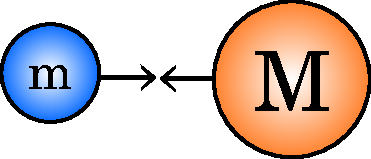
\includegraphics[width=.7\linewidth]{images/gravitational.pdf}
    \caption{Gravitation}
  \end{subfigure}%
  \begin{subfigure}{.5\textwidth}
    \centering\captionsetup{width=.9\linewidth}%
    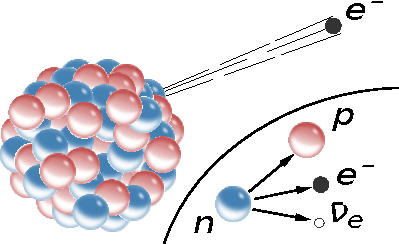
\includegraphics[width=.6\linewidth]{images/weak.pdf}
    \caption{Weak Interaction\cite{WeakForce:2021}}
  \end{subfigure}
  \begin{subfigure}{.5\textwidth}
    \centering\captionsetup{width=.9\linewidth}%
    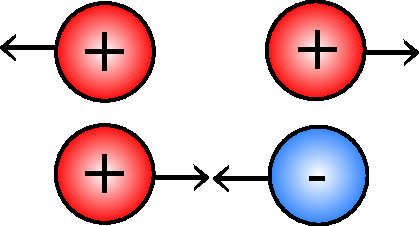
\includegraphics[width=.7\linewidth]{images/em.pdf}
    \caption{Electromagnetism}
  \end{subfigure}%
  \begin{subfigure}{.5\textwidth}
    \centering\captionsetup{width=.9\linewidth}%
    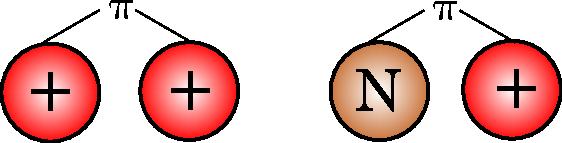
\includegraphics[width=.6\linewidth]{images/strong.pdf}
    \caption{Strong Interaction}
  \end{subfigure}
  \caption{The four fundamental forces}
  \label{fig:4forces}
\end{figure}

The Standard Model attempts to describe the particle physics phenomena through the unification of the fundamental forces at a sub-atomic level
(gravitational interaction, owing to its negligible effect on elementary particles, can be ignored at presently accessible energies)\cite{ShawMartin:2017}.
The inclusion of the the three fundamental forces in the model are described by their respective theoretical frameworks:
\begin{itemize}
  \item The electromagnetic interaction is described through Quantum Electrodynamics (QED)
  \item The strong interaction is described through Quantum Chromodynamics (QCD)
  \item The weak interaction can be described by electroweak unification, combining weak nuclear force with Quantum Electrodynamics
\end{itemize}

The strong interaction, aptly named being relatively the strongest of the four interactions, but with a short range, extends over the femtometer range
binding the quarks within the nucleons and the nucleons within the nucleus itself. It is also responsible for generating most of the mass of hadrons,
interacting between the color charges and described by Quantum Chromodynamics.

The electromagnetic interaction, whose electric and magnetic phenomena can be observed on a macroscopic scale, acts on all particles possessing an
electromagnetic charge. With an infinite range and second in strength after the strong interaction, the theoretical framework describing the EM
interaction is outlined by Quantum Electrodynamics.

The weak interaction, documented by the decay of unstable particles, is weaker in strength than the Strong and EM interactions, owing to heavier
force-carrier particles resposible for the interaction (\textsl{W} and \textsl{Z} bosons). Energies in excess of mass of these bosons render EM and
weak interactions with a comparative strength, and clubbed together, they are explained by the unified theory of electroweak interactions. The theory
also incorporates the Higgs field and the Higgs mechanism, reponsible for mass generation in elementary particles.

The gravitational interaction, relatively being the weakest of the four forces, has an infinite range acting over all massive particles and can
be described by Einstein's general theory of relativity. Due to its infinitesimal impact on the sub-atomic scale when compared to the other three
forces, it is not a part of the Standard Model. However, on a macroscopic scale, gravitational interaction holds a much more
significant position, prevailing over the short-ranged strong and weak nuclear forces, while most electromagnetic interactions are screened due
to electrically neutral nature of atoms.

The Standard Model also sheds light on the origin of these forces, especially relevant at short distances when quantum effects become significant. This
assertion is based on particle interaction through an exchange of force-carrier particles classified as gauge bosons, a subset of bosons - a broader
class of particles described further in this section. Each fundamental force is
described by its corresponding gauge boson responsible for discrete energy transfer. Table \ref{tab:GriffithsSmTable} lists the four fundamental
forces and their theoretical frameworks, their comparative strengths and corresponding gauge bosons.

\begin{table}
  \centering
  \begin{tabular}{lrll}
    Force           & Strength   & Theory           & Mediator\tabularnewline
    \hline
    Strong          & 10         & Chromodynamics   & Gluon\tabularnewline
    Electromagnetic & 10$^{-2}$  & Electrodynamics  & Photon\tabularnewline
    Weak            & 10$^{-13}$ & Flavourdynamics  & \textsl{W} and \textsl{Z}\tabularnewline
    Gravitational   & 10$^{-42}$ & Geometrodynamics & Graviton\tabularnewline
    \hline
  \end{tabular}
  \caption{The four fundamental forces\cite{GriffithsSmTable:2008}}
  \label{tab:GriffithsSmTable}
\end{table}

Primarily, the Standard Model classifies elementary particles into two main classes: \textit{bosons} and \textit{fermions}. Fermions, regarded as the
building blocks of matter, exist in 24 variants including their particle and anti-particle counterparts. The elementary fermions are subdivided
into quarks and leptons, each with a unique mass, ${\textstyle \frac{1}{2}}$ spin value (thus obeying the Pauli exclusion principle), and an
electrical charge (except for the electrically neutral neutrinos). The antiparticle counterparts carry over the same mass but opposite quantum
numbers (electrical charge, lepton number, etc.). Although the fermions exhibit the same electric charge and similar interaction capabilities for the
weak and strong nuclear forces across the three generations, the primary difference noted among the generations lies in their increasing trend of
average mass (Fig. \ref{fig:SmElementaryParticles}) depending on their coupling with the Higgs field.
Fermions obey the Fermi-Dirac statistics, and combine together to form composite particles such as hadrons, nuclei and atoms, which can be bosonic or fermionic in their nature depending
on the constituents involved.


\begin{figure}[H]
  \centering
  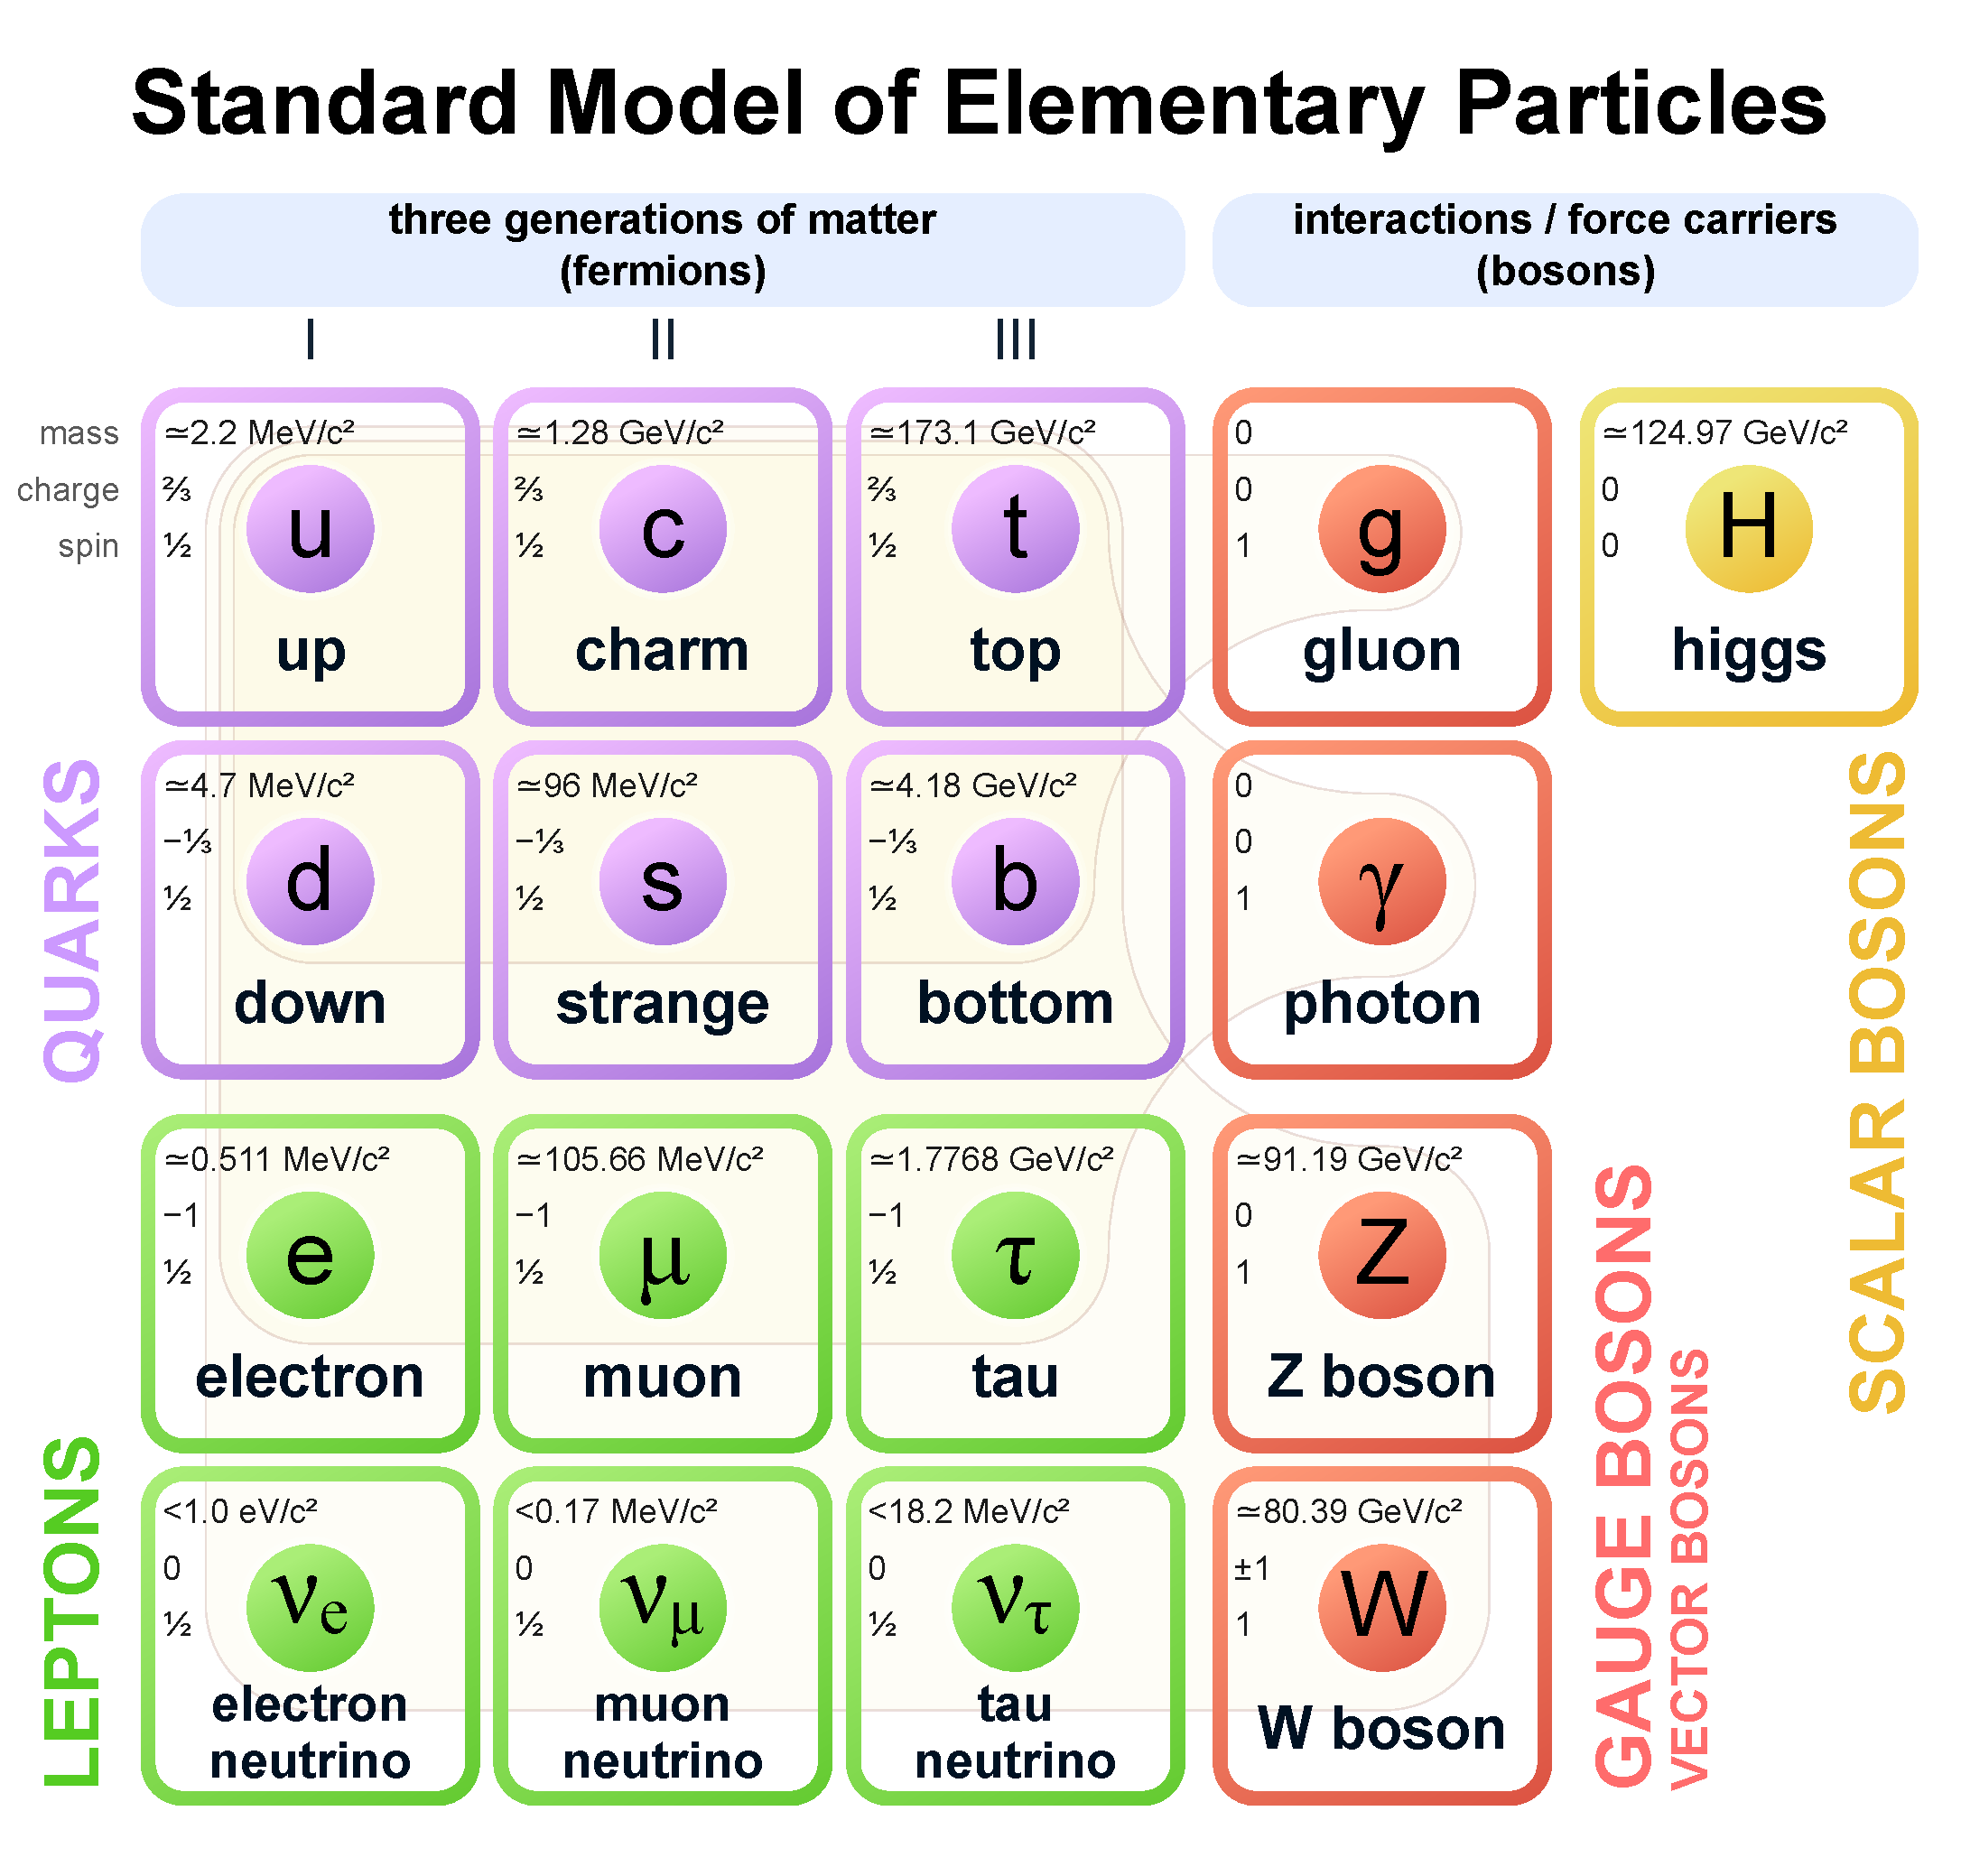
\includegraphics[width=0.9\linewidth]{images/SmElementaryParticles.pdf}
  \caption{Standard Model of Elementary Particles\cite{SmElementaryParticles}. Corresponding antiparticles exist for all listed particles,
    except for $g, \gamma, Z^{0}$ and $H$ (which are their own antiparticles).}
  \label{fig:SmElementaryParticles}
\end{figure}


Bosons, on the other hand, have integer spin values (spin-0 or spin-1) which exempts them from the Pauli exclusion principle. Currently, the Standard
Model encapsulates five different bosons, out of which four of them are known as gauge bosons (spin-1) which act as the force-carriers for the
aforementioned three fundamental forces. The gluon (\textit{g}) acts as the mediator for the strong interaction, photon (\textit{$\gamma$}) for the
electromagnetic interaction and the \textit{W$^{\pm}$} and \textit{Z$^{0}$} bosons act as mediators for the weak interaction. The fifth boson, scalar
in nature with a spin-0 value, is a recently discovered member to the Standard Model. This particle, known as the Higgs boson, is deemed to be
responsible for assigning mass to particles. Bosons follow the Bose-Einstein statistics for the formation of composite particles.

\begin{figure}
  \centering
  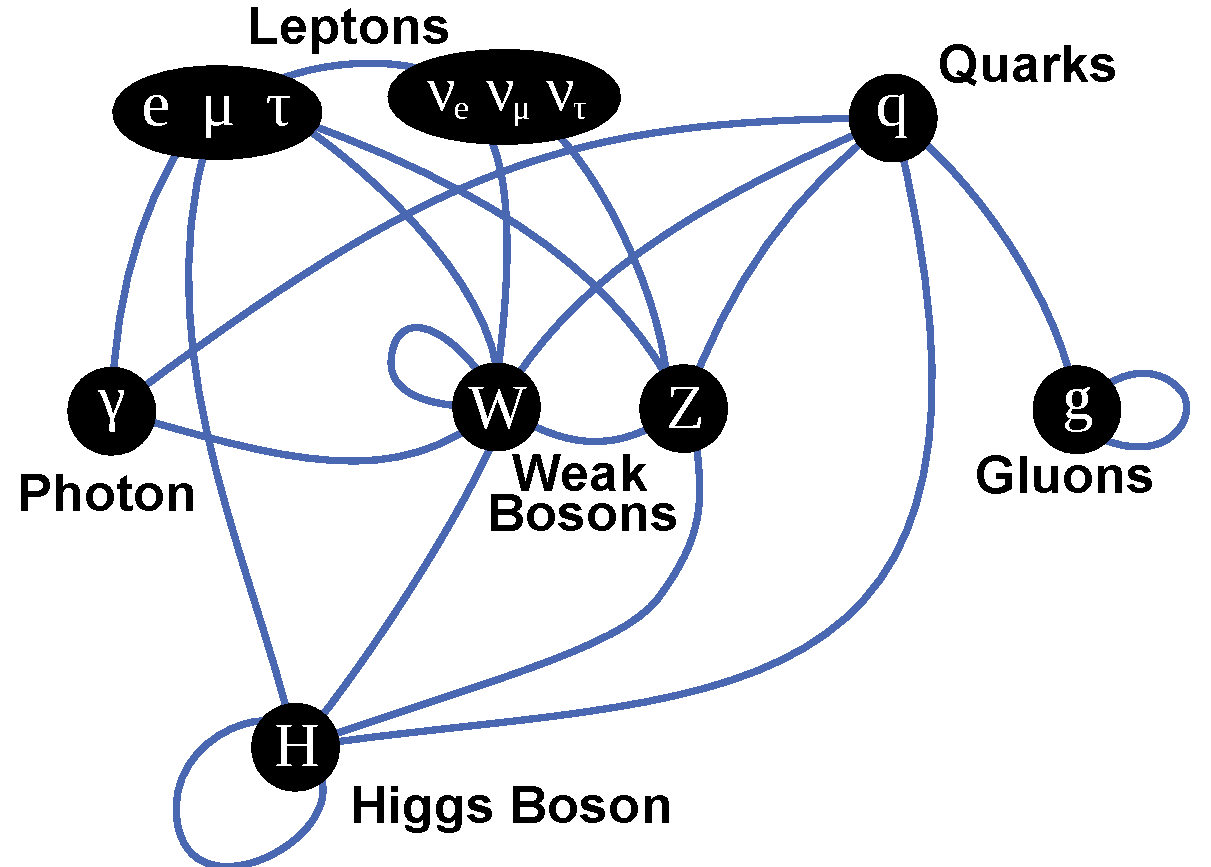
\includegraphics[width=0.75\linewidth]{images/ElementaryParticleInteractions.pdf}
  \caption{Interactions between Elementary Particles\cite{ElementaryParticleInteractions}}
  \label{fig:ElementaryParticleInteractions}
\end{figure}


The interactions among elementary particles and their combinations are outlined in Fig. \ref{fig:ElementaryParticleInteractions}, with closed curves
depicting interactions within the
group. The Higgs boson interacts with itself and all massive particles, the quarks interact via strong interaction with all bosons and particles
possessing a 'colour' charge. Gluons exhibit quark-gluon interaction alongwith self-interaction, which is discussed further in the next sections.

\section{Quantum Chromodynamics}
Quantum Chromodynamics (abbreviated as 'QCD') is a theoretical framework that aims to explain the mechanics of the strong interaction, alongwith the
fundamentals pertaining to the nature and conduct of quarks and gluons (collectively known as partons). Apart from the aforementioned attributes of
unique mass and an electrical charge, QCD defines partons to possess an additional quantum number known as 'colour' charge. The concept of colour
charge was first put forward by Oscar W. Greenberg\cite{OWG:1964}, M. Han and Y. Nambu\cite{HanNambu:1965}, justifying the coexistence of quarks in
identical quantum states bound in hadrons without violating Pauli's
exclusion principle. As an example, the discovery of delta baryon --  $\Delta^{++}$ (u,u,u) consisting of three up quarks with parallel spin could
be validated.

The colour quantum number exists in three equivalent states, dubbed as red, green and blue. Much like its electromagnetic counterpart, each colour
charge has its corresponding antiparticle colour state (Fig. \ref{fig:colorCharge}); and similar to the photon's coupling to the electromagnetic
charge in QED, the gluon couples to the colour charge in QCD. However, unlike the photon, the gluon carries the charge of the colour it mediates,
thereby enabling self-interaction while also participating in the strong interaction. Contrary to quarks which carry a single colour charge, gluons
carry both the colour and anti-colour charge. The gluon-gluon and gluon-quark interactions maintain the conservation of colour charge. The colour
charge is also confined, i.e. the colour charged particles cannot be isolated and must remain in conjunction as colourless hadrons (also stated as
colour-singlets) below the Hagedorn temperature ($\sim10^{12} K)$. This phenomenon is termed as colour confinement\cite{FlorkowskiColour:2010} and is
responsible for the absence of free quarks and gluons.

\begin{figure}[H]
  \centering
  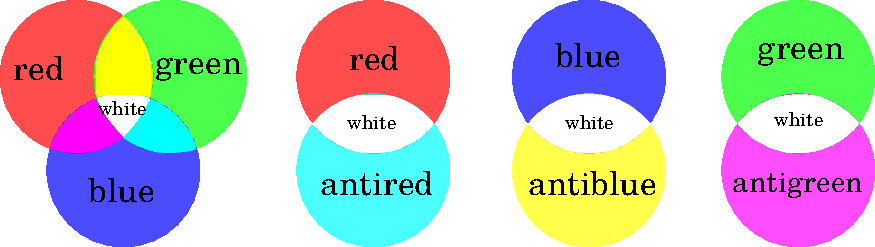
\includegraphics[width=0.7\linewidth]{images/colorCharge.pdf}

  % \textit{Baryons\hspace{6.5cm}Mesons}
  \caption{An illustration depicting the colour charges and their combinations. Baryons are composed of red, green and blue colour charges (left),
    while a singular pair of colour-anticolour combination forms a meson, as shown in the last three diagrams.}
  \label{fig:colorCharge}
\end{figure}

The gluon self-interaction causes anti-screening due to quantum fluctuations, and the probability for this effect increases with distance between
quarks. This effect gives rise to a phenomenon known as asymptotic freedom\cite{Gross:1973,Politzer:1973}, indicating that larger distances between interacting
quarks lead to increased strength of the strong interaction. The strength of the strong interaction can be measured by its running coupling constant
$\alpha_{s}$, which can be defined as follows\cite{FlorkowskiCoupling:2010}:

\medskip
\begin{equation}
  \alpha_{s}(Q^{2})=\frac{16\pi^{2}}{(11 - \frac{2}{3}N_{f})ln(\frac{Q^{2}}{\Lambda_\textnormal{\sc qcd}^{2}})} \hspace{0.15cm} \xrightarrow{Q^{2}\to\infty} 0,
  \label{eq:CouplingQCD}
\end{equation}
\smallskip

where Q is the Lorentz invariant generalisation of momentum transfer, $N_{f}$ is the number of included quark flavours that can partake in the
screening loop and $\Lambda_\textnormal{\sc qcd}$ is the QCD scale parameter determined either experimentally or from lattice QCD calculations such that the
coupling constant is calibrated at mass of $Z^{0}$ boson ($\Lambda_\textnormal{\sc qcd} \approx 200$ MeV). From the experimental results (Fig. \ref{fig:CouplingQCD}),
the dependence of $\alpha_{s}$ on $Q$ can be confirmed. At short distances, the
coupling constant vanishes, implying that parton interactions are negligible in the limit of very high temperatures\cite{Gross:1973,Politzer:1973}.
This occurrence points to the creation of a virtually non-interacting QGP at extreme temperatures\cite{Collins:1975,Cabibbo:1975}.

\begin{figure}[H]
  \centering
  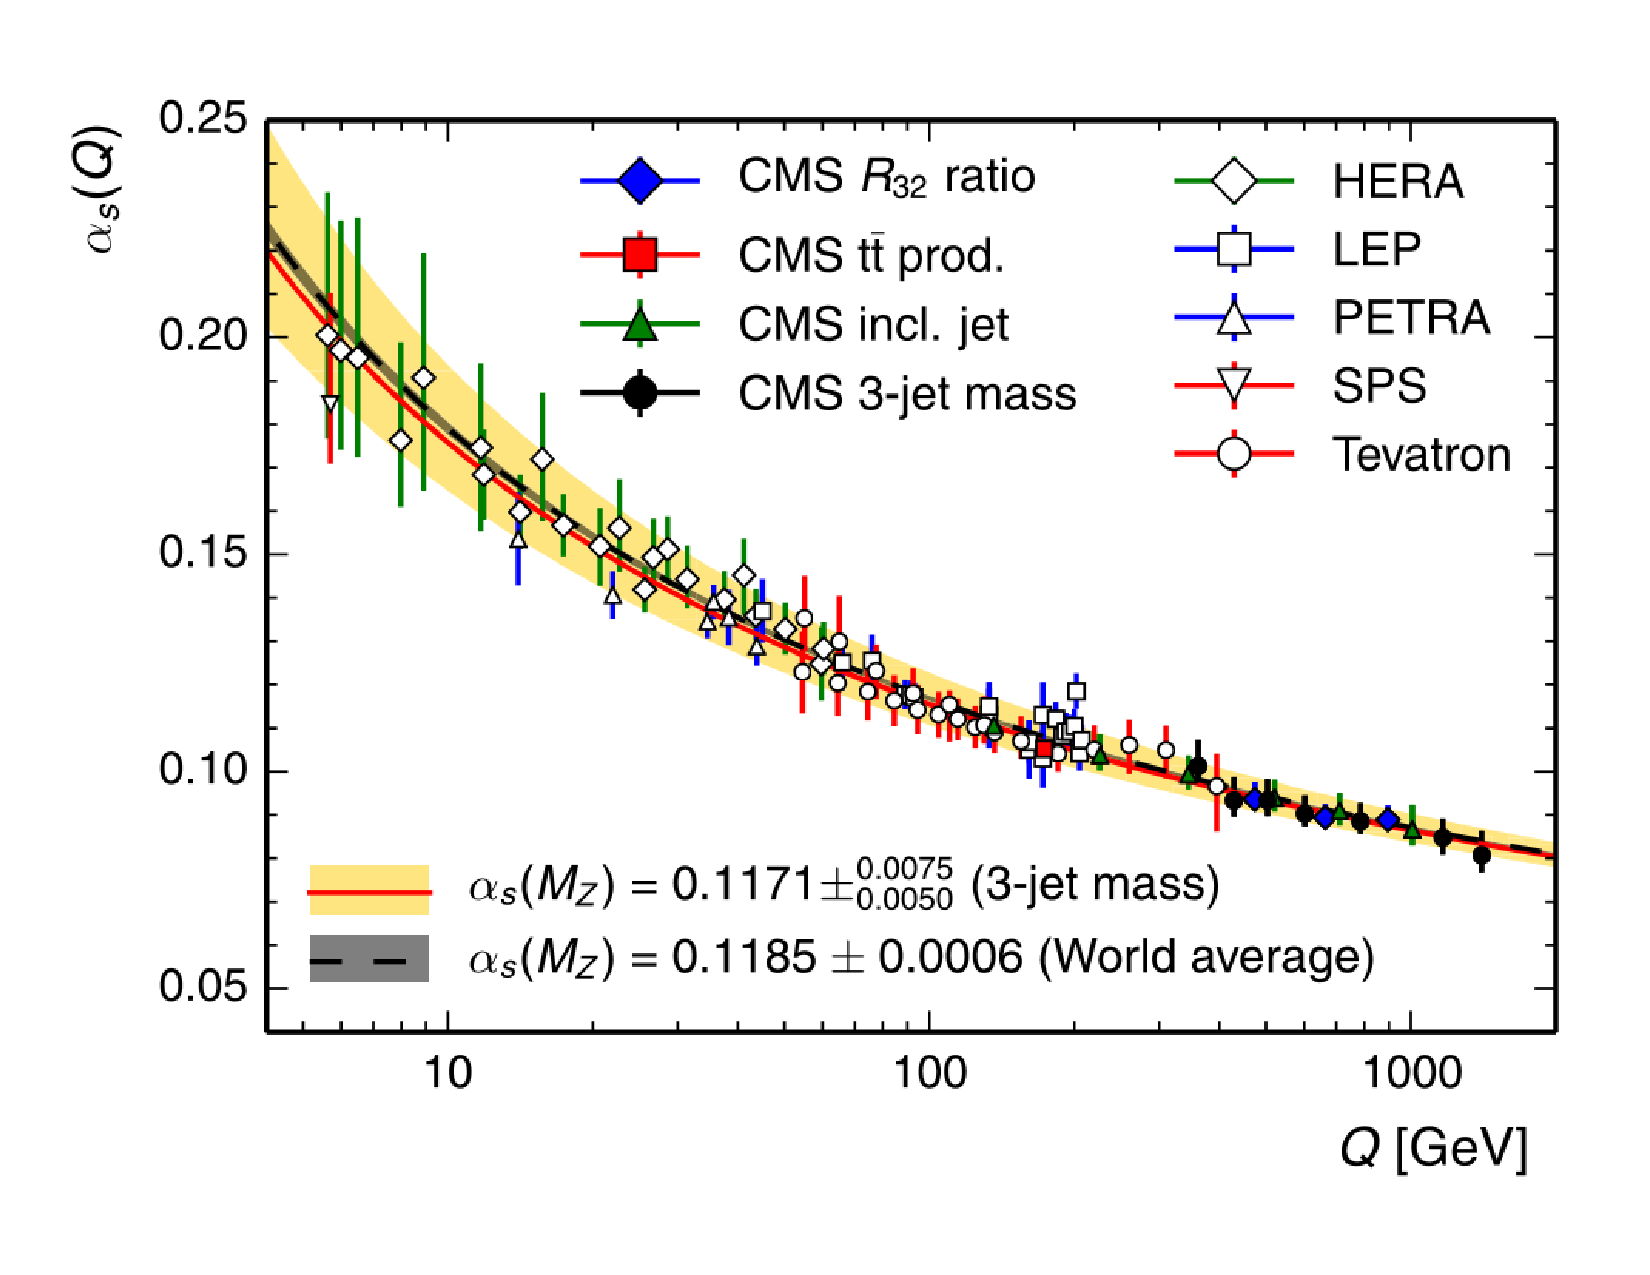
\includegraphics[width=0.7\linewidth]{images/CouplingQCD.pdf}
  \caption{Comparison of $\alpha_{s}$ evolution as measured by different experiments\cite{CouplingQCD:2015}.}
  \label{fig:CouplingQCD}
\end{figure}

\section{Quark-Gluon Plasma}

As stated earlier, the phenomenon of colour confinement points to a bound state of quarks and gluons within hadrons in ordinary circumstances.
However, the existence of a phase consisting of deconfined quarks and gluons achieved by high temperatures and/or significant net baryon densities
has been hypothesised early on and presumed to exist in neutron stars and the early universe, shortly after the Planck epoch\cite{PlanckEpoch} according to the Big Bang
theory\cite{bigBang}.
Attempts to recreate this primordial liquid have been carried out by various particle accelerators and collider experiments making use of
immense pressure values to 'merge' the hadrons together and creating high enough temperatures to excite quarks out of their bound state in hadrons.
The extreme temperature ($\sim 1.97\times10^{12}$ K) and particle density should result in the merging of confined partons to an incredibly hot,
superdense quark-gluon 'soup' (Fig.\ref{fig:qgp}), where free quarks could exist. Particle collisions at the Large Hadron Collider are believed
to exhibit conditions sufficient for the creation of this new state of matter.

\begin{figure}[H]
  \centering
  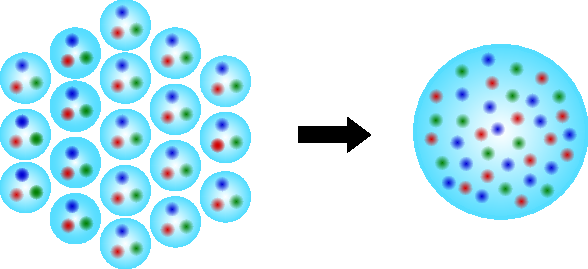
\includegraphics[width=0.7\linewidth]{images/qgp.pdf}
  \caption{An illustration depicting isolated hadrons merging into a quark-gluon plasma.}
  \label{fig:qgp}
\end{figure}

Although named as a plasma based on the assumption that the QGP would be exhibiting properties akin to an ultrahot gas of charged particles, the
quark 'soup', in essence, behaves as a nearly perfect Fermi liquid: the strongly coupled QGP (sQGP)\cite{HeinzRHIC:2005}. Models based on relativistic
hydrodynamics at the LHC and RHIC have been able to effectively describe the fluid-like characteristics and related observables like elliptic flow,
radial expansion and higher order flow harmonics.

The grand canonical ensemble characterises nuclear matter in thermodynamic equilibrium with respect to temperature $T$, volume $V$, and the
baryo-chemical potential $\mu_\textnormal{\sc b}$. Here, $\mu_\textnormal{\sc b}$ is the chemical potential of the conserved baryon number. Figure \ref{fig:QcdPhaseDiagram}
depicts a schematic representation of the phase diagram of nuclear matter in the $\mu_\textnormal{\sc b}, T$ plane. Nuclear matter, ordinarily, exists at
$T\approx0$ and $\mu_\textnormal{\sc b}\approx1$ GeV. The phase boundary ending in a critical end-point differentiates the hadron resonance gas phase from the
quark-gluon plasma. For a critical point $E$ on the diagram, lattice QCD approach determines $T_\textnormal{\sc e}\approx160$ MeV and $\mu_\textnormal{\sc e}\approx725$ MeV\cite{Fodor:2002}.
At minimal $\mu_\textnormal{\sc b}$ values,
the critical temperature for transition's cross-over is ($T_\textnormal{\sc c}\approx170$ MeV). On the other hand, at low values of temperature but baryon density
exceeding a few times of nuclear matter density, a deconfined color superconducting phase is predicted, perhaps along with other phases\cite{Fukushima:2013}.

According to recent lattice calculations, a slightly lower transition temperature ($T_\textnormal{\sc c}\approx155$ MeV) is forecasted\cite{Bazavov:2012, Bhattacharya:2014},
which agrees well with the statistical hadronisation model's chemical freeze-out temperature\cite{Andronic:2009}.

\begin{figure}
  \centering
  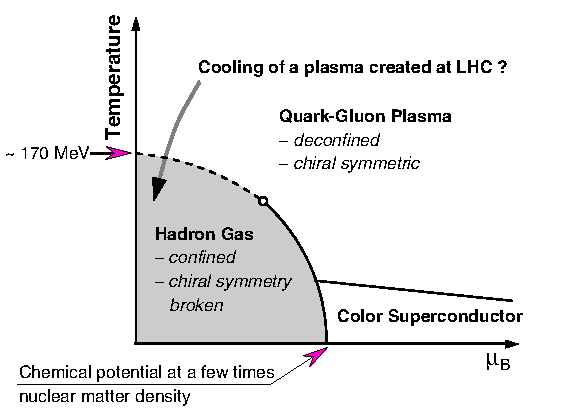
\includegraphics[width=0.8\linewidth]{images/QcdPhaseDiagram.pdf}
  \caption{\small The phase diagram of QCD: solid lines indicate first-order transitions, dashed lines indicating possible continuous rapid
    crossover transition\cite{Carminati:2004}.}
  \label{fig:QcdPhaseDiagram}
\end{figure}


The QGP state, by itself, is quite unstable owing to the extreme conditions required for its creation and sustainability, hence it exists for a
microscopic amount of time before cooling down and re-confining back to the hadron state. At LHC energies, the expected lifetime of QGP is
judged to be 4 to 6 fm/c\cite{Sahoo:2010}, hence any observation for its formation are required to be probed in this interval or at the
earliest collision moment so as to avoid any subsequent hadronisation. This presents a challenge to make direct observations for QGP's existence
owing to its limited lifetime to verify its creation on a macroscopic scale.
Therefore, its existence and effects must be studied indirectly by observing the auxiliary phenomena as signatures of QGP\cite{Bass:1999}$\colon$
\begin{enumerate}
  \item Production of direct (thermal) photons and thermal dileptons
  \item Suppression of J/$\psi$ and $\psi^{\prime}$ particle production
  \item Increased yield of strange and multi-strange hadrons
  \item Jet Quenching
  \item Suppression of the production of hadrons with high transverse momentum
  \item Collective (Elliptic, directed, and transverse) flow of baryons and mesons
  \item Increased baryon production at mean transverse momentum
  \item Change in the mass and lifetime of vector mesons
\end{enumerate}

In this thesis, the increased yield of multi-strange baryons in high energy collisions is studied. The production of multi-strange cascade baryons
such as $\Xi^{\pm}$ and $\Omega^{\pm}$ in p-Pb collisions at LHC energies $\sqrt{s_{\textnormal{\sc nn}}}$ = 8.16 TeV in the ALICE detector are presented. An overview
comprising of the theoretical and experimental advancements in the realm accompanied by the importance of strangeness studies in strongly interacting
matter and as a signature of the quark-gluon plasma is discussed. Analysis details, consisting of the detector layout and important sub-detectors
pertaining to the data collection and particle information necessary for analysis, data sample, processing, analysis and filtering
to obtain good candidates for reconstruction, subsequent analysis methods and follow up tasks are explained. Summing up with the current status of
the analysis and raw $p_{\textnormal{\sc t}}$ spectra results, the final goals and outlook is presented.




\chapter{Experimental results preview}

Since its introduction, the theory of perturbative Quantum Chromodynamics (pQCD) has made huge strides and its calculations for the strong coupling constant
are improving by the inclusion of higher order terms in the power series. However, the non-perturbative regime is still poorly understood as numerical
calculations on a lattice fail to describe dynamical factors such as transport coefficients and cross sections, as opposed to outlining light nuclei
and hadron spectra. Therefore, to further the understanding of QCD under extreme temperatures and baryon densities, experiments involving high energy
particle collisions pave the way for development of new theoretical tools to describe the phenomena in a new light.

\section{Ion collider experiments}
The experimental endeavours in the search for a deconfined state of matter began as early as 1986 with fixed target experiments at the Alternating Gradient
Synchrotron (AGS) at Brookhaven National Laboratory (BNL) and the Super Proton Synchrotron (SPS) at CERN. Beginning with light atomic nuclei like $^{16}$O,
$^{28}$Si and $^{32}$S, the focus of the experiments shifted towards heavier nuclei collisions involving $^{197}$Au and $^{208}$Pb in the 1990's. The
AGS demonstrated centre-of-mass energy per colliding nucleon pair of $\sqrt{s_{\textnormal{\sc nn}}}$ = 4.6 GeV while the SPS achieved
$\sqrt{s_{\textnormal{\sc nn}}}$ = 17.2 GeV in Pb-Pb collisions\cite{MunzingerStachel:2007} and $\sqrt{s_{\textnormal{\sc nn}}}$ = 19 GeV in S-S
collisions\cite{Evans:1999}. The results from SPS experiment at CERN gathered enough evidence to conclude a new state of matter had been
created\cite{SPSqgp:2000, HeinzLHC:2000}.

Concurrently, a new accelerator with much higher collision energies went into operation at BNL. The Relativistic Heavy-Ion Collider (RHIC) made it possible
to reach centre-of-mass energies $\sqrt{s_{\textnormal{\sc nn}}}$ = 200 GeV by colliding heavy nuclei such as gold and servicing four experiments called
BRAHMS, PHENIX, PHOBOS and STAR. The higher collision energies reached at RHIC meant a significantly larger and hotter fireball was possible. From the
experiments at RHIC, it was concluded that QGP is not a gas-like plasma but is a strongly interacting near-perfect fluid\cite{Adams:2005}.

The initiation of LHC set a new world-record for heavy ion collisions at $\sqrt{s_{\textnormal{\sc nn}}}$ = 2.76 TeV per nucleon for Pb-Pb during its first
run (2010--2013), and $\sqrt{s_{\textnormal{\sc nn}}}$ = 5.02 TeV per nucleon for Pb-Pb during Run 2 (2015--2018). This allowed a deeper study of the QGP
phase and its properties owing to more extreme conditions and a detailed characterisation of hadronisation and particle generation as the fireball cools down.
An in-depth overview of the LHC and the ALICE experiment focusing on QGP study is provided in Chapter \ref{sec:LHC}.

\section{Experimental Observables}

Since the QGP cannot be observed directly at present, external observables are used to gauge information about the particles produced in the
collisions. These observables, called probes, can be categorised into two types: soft and hard probes. Soft probes characterise the macroscopic and
collective behaviour of particles and the collision as a whole, while hard probes allow energy loss studies within the QGP and are sensitive to strong
interaction at the partonic level.

\subsection{Collective flow and correlations}
Anisotropies observed in the final momentum distribution of particles created in nuclear collisions suggest the presence of collective behaviour in the
formed system. Initially proposed as a signature of QGP's collective behaviour, in-plane elliptic flow was experimentally observed at
AGS\cite{FlowAGS:1994} and SPS\cite{FlowSPS:2003}. A strong elliptic flow measured at RHIC clarified QGP's resemblance to a strongly interacting
liquid\cite{Adams:2005}.

The initial overlap region of colliding nuclei plays a major role in anisotropies in momentum distribution as different pressure gradients form along
different axes. These anisotropies can be quantified using the Fourier coefficients of the azimuthal particle distributions:

\begin{equation}
    v_{n} = \langle cos[n(\phi - \Psi_{n})]\rangle
    \label{eq:fourier}
\end{equation}

where $n$ is the flow harmonic order, $\phi$ is the azimuthal angle of the particle, and $\Psi_{n}$ is the angle of the initial state spatial plane of
symmetry\cite{Voloshin:1996, Fourier:2011}. The first, second and third harmonics indicate directed, elliptic and triangular flow respectively.
The elliptic flow coefficient $v_{2}$ signifies the difference between pressure gradients, although higher order coefficients also help in decrypting
the initial state geometry and the fireball's evolution.

Flow measurements allow constraints to be put on equation of state and enable kinematic viscosity measurements, $\eta/s$, defined as ratio of shear
viscosity to entropy density. $\eta/s$ value for a perfect fluid has a lower limit of $\frac{1}{4\pi}$\cite{Viscosity:2005}(natural units). Experimental
values from RHIC and ALICE, LHC are consistent with $\eta/s$ = 0.12 and $\eta/s$ = 0.2 respectively\cite{Gale:2013} (Fig. \ref{fig:viscosity}). The low $\eta/s$ values
point towards QGP's status as a near-perfect fluid and differences between results from RHIC and ALICE allow determination of temperature dependence of
kinematic viscosity.
\begin{figure}[H]
    \centering
    \begin{subfigure}{.5\textwidth}
        \centering
        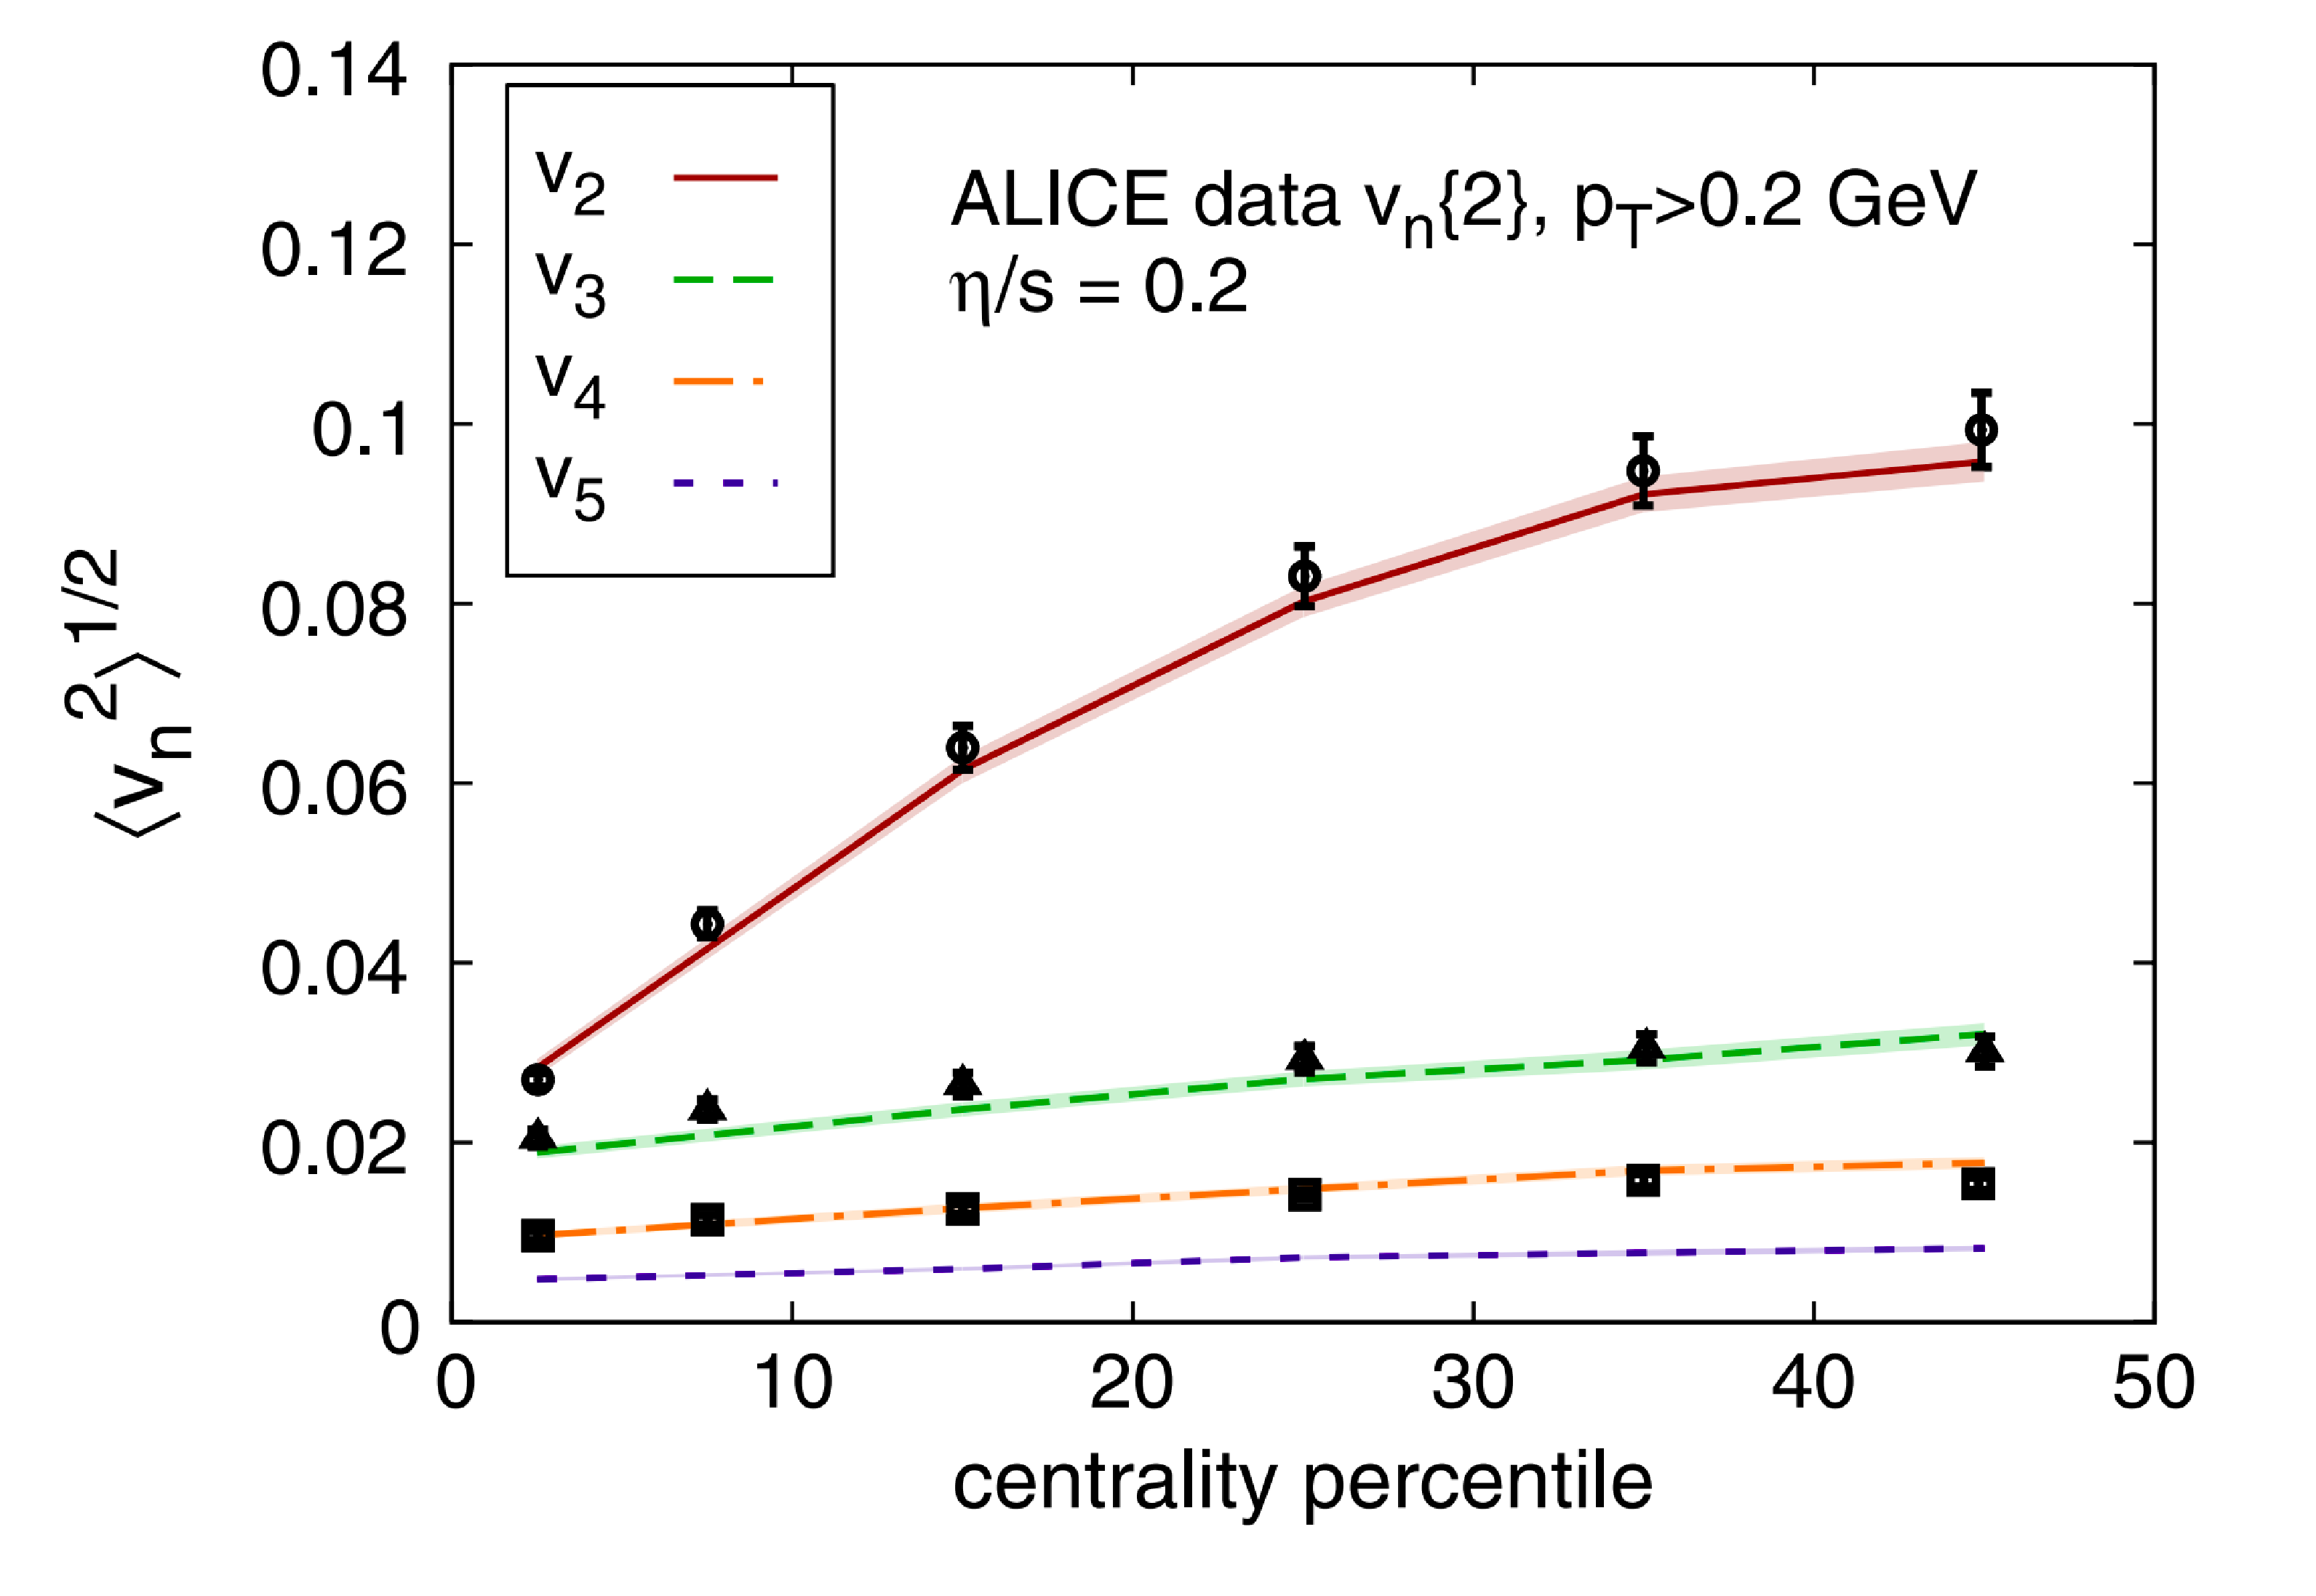
\includegraphics[width=\linewidth]{images/aliceViscosity.pdf}
    \end{subfigure}%
    \begin{subfigure}{.5\textwidth}
        \centering
        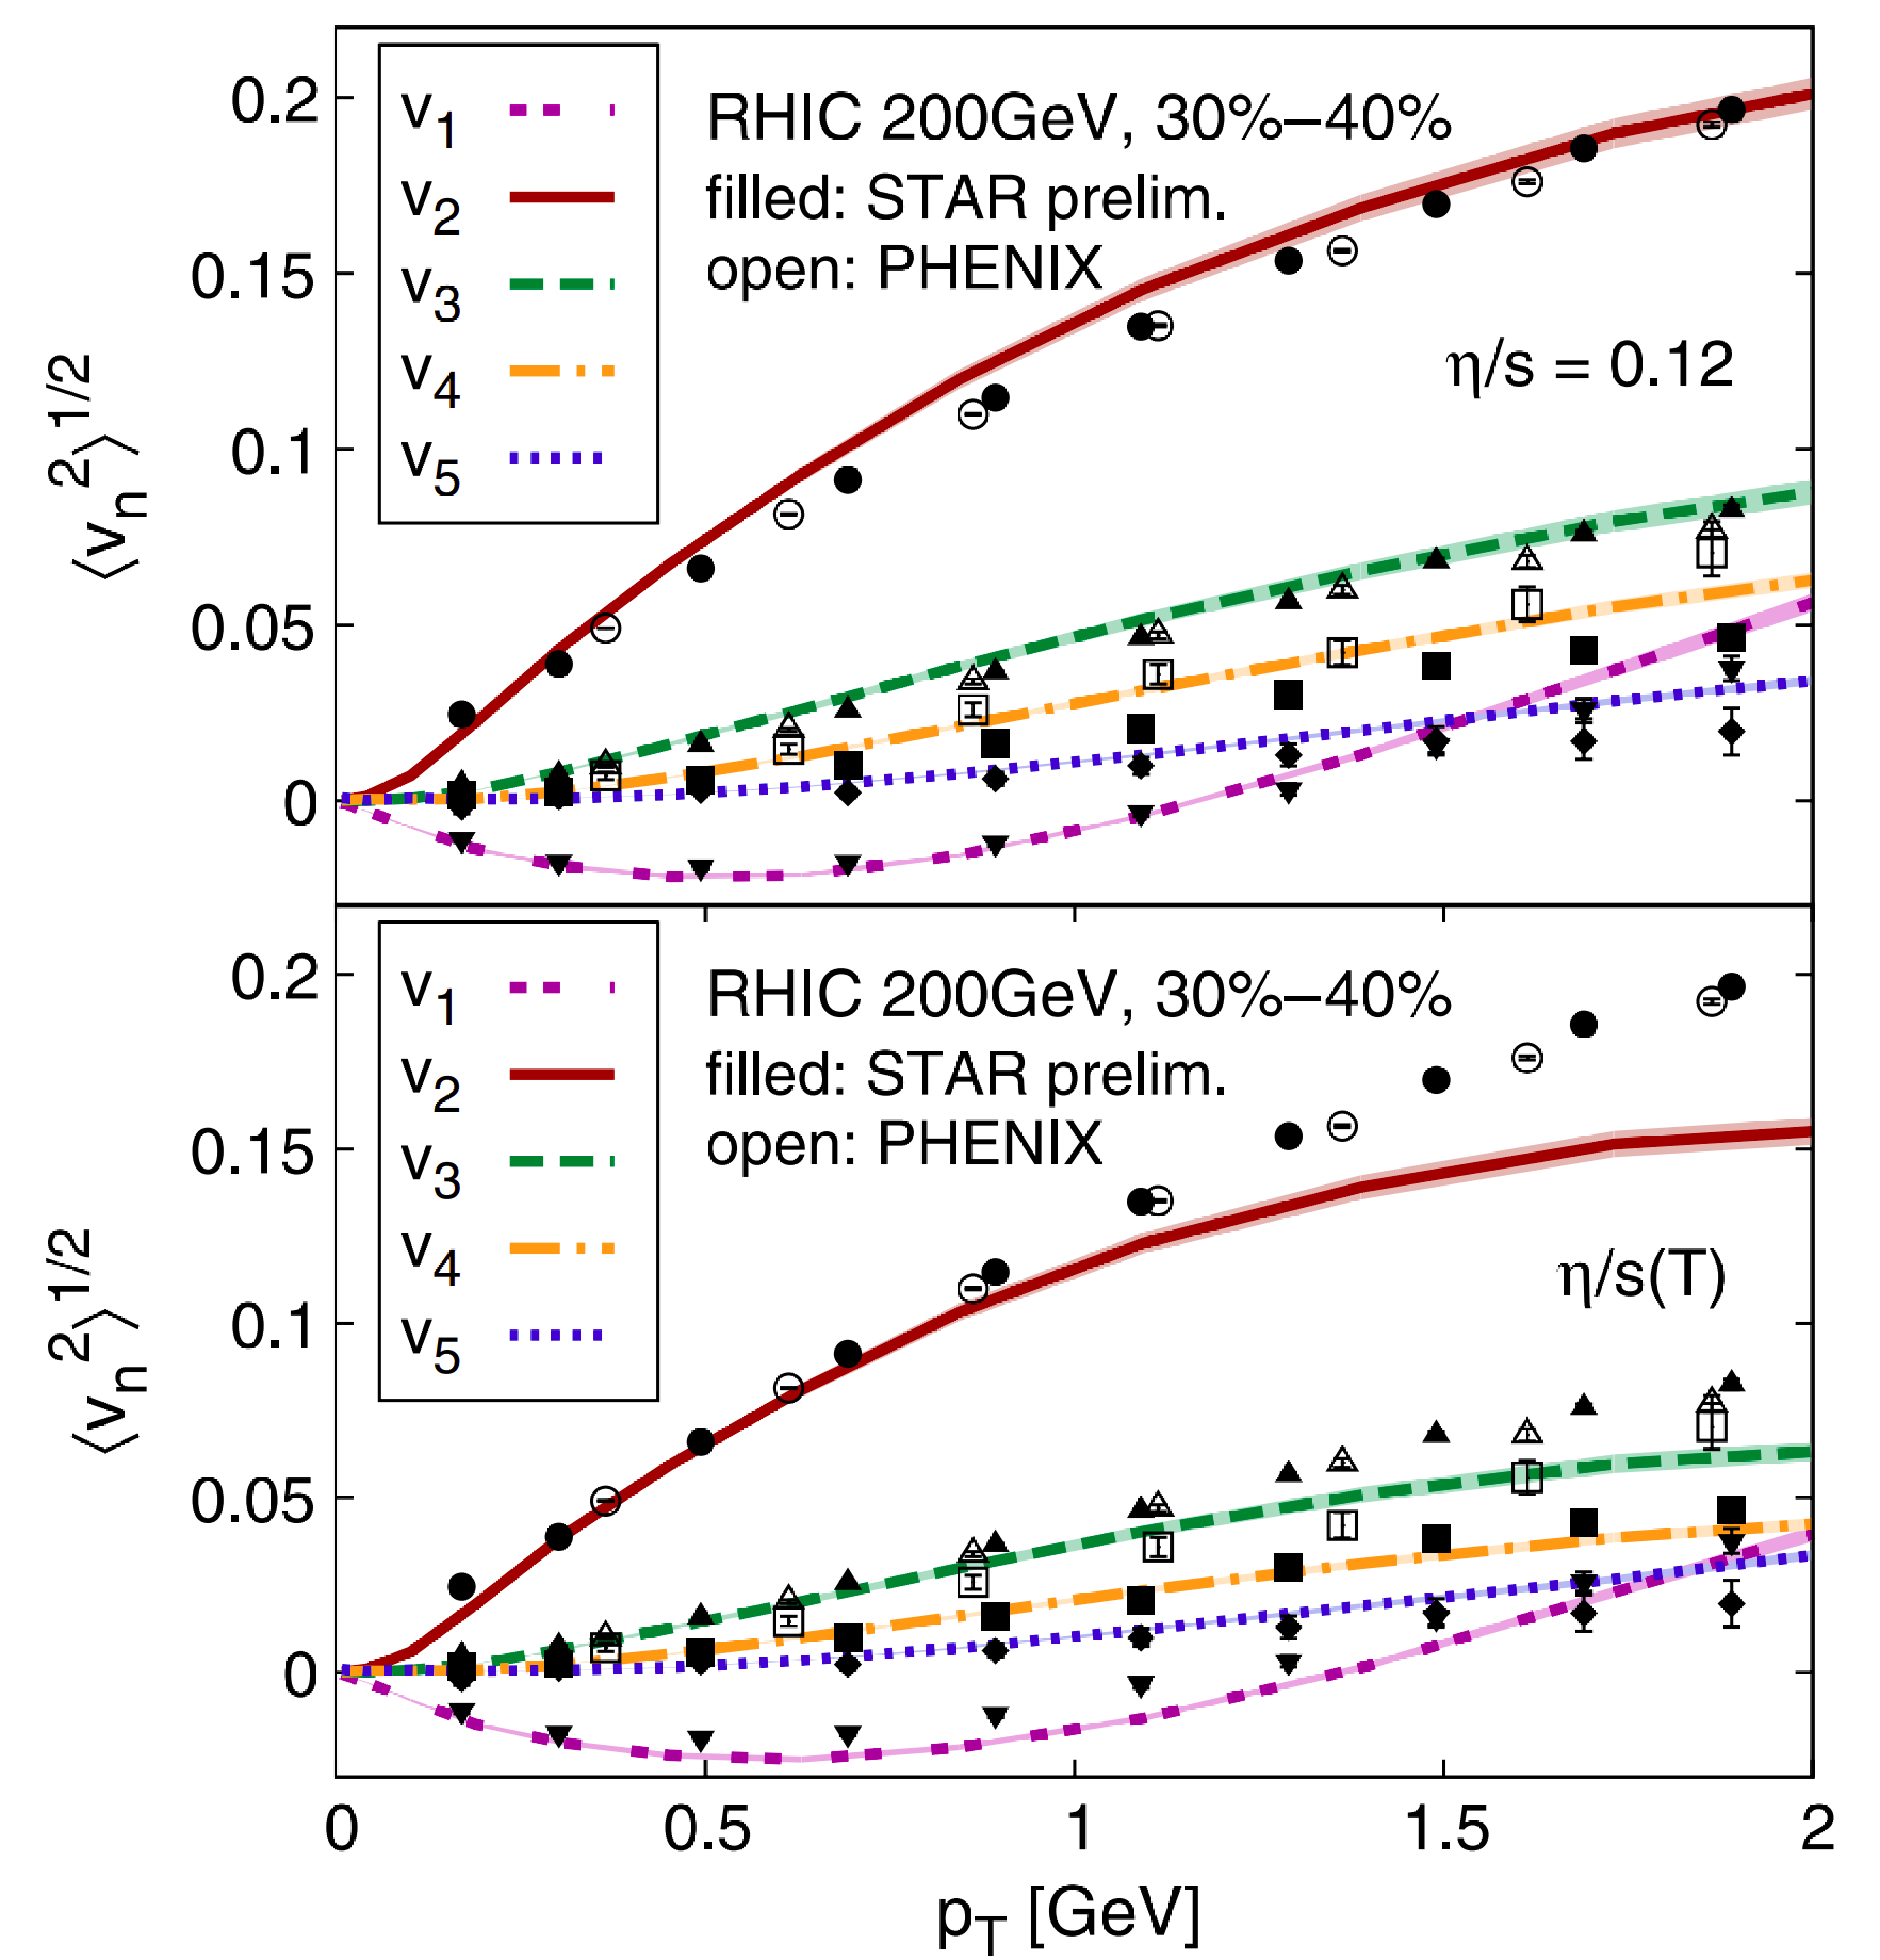
\includegraphics[width=\linewidth]{images/rhicViscosity.pdf}
    \end{subfigure}
    \caption{RMS values of anisotropic flow coefficients $\langle v_{n}^{2}\rangle^{1/2}$. Left plot from ALICE Collaboration depicts $\langle v_{n}^{2}\rangle^{1/2}$
        computed as a function of centrality\protect \footnotemark \ and compared to experimental data based on $v_{n}\{2\}, n\in 2,3,4$. Plot on the right from the PHENIX and 
        STAR collaboration shows a comparison
        of $v_{n}(p_{\textnormal{\sc t}})$ at RHIC using a constant $\eta/s$ = 0.12 (top) and a temperature
        dependent $\eta/s$(T) (bottom)\cite{Gale:2013}.}
    \label{fig:viscosity}
\end{figure}
\footnotetext{centrality of a collision is expressed as a percentage of total nuclear interaction cross section}

When deviating from central collisions, the overlap region of the colliding nuclei becomes less circular and more almond shaped. This increase in spatial
anisotropy results in an increased elliptic flow, as seen in LHC's measurements in Fig. \ref{fig:viscosity} on the left. Higher LHC energies enable elliptic flow to be examined
in detail, in conjunction with higher flow harmonics which can shed a light on initial collision conditions and viscosity of the medium.

\subsection{Jet quenching}

In a hard scattering process (high momentum transfer), the fragmentation of a highly energetic parton results in a collimated spray of hadrons called a
jet. The involved partons, after scattering and hadronization, retain a significant amount of the initial beam momentum and are thus emitted in a narrow
"jet cone". A jet cone can be experimentally identified as a stream of high energy particles moving in approximately the same direction. The hadron in a
jet carrying the highest value of energy is called the leading particle of the jet.

Jet quenching refers to the collisional or radiative energy loss of high energy partons when passing through a hot and dense medium, such as the QGP. The
resulting lower than expected momenta of hadrons produced through hard scattering events leading to a suppression of jets in heavy ion collisions has been
proposed as a key signature of QGP formation\cite{Bjorken:1982}. Various factors determine the energy loss of the jet including the type of parton (quark
or gluon), its energy and mass, the mechanism of energy loss (collisional or radiative), and also medium-induced factors such as the path length and properties
of the medium (size, temperature, coupling). Collisional energy loss occurs due to elastic parton-parton scattering involving a high energy parton, while
radiative energy loss is due to medium-induced gluon radiation.

Experimentally, parton energy loss can be observed through suppression of jet and leading particle spectra by comparing nuclei collision results (QCD medium)
with proton collision results (QCD vacuum). This ratio is stated as the nuclear modification factor, $R_{\textnormal{\sc aa}}\colon$

\begin{equation}
    R_{\textnormal{\sc aa}} \sim \frac{\textnormal {QCD Medium}}{\textnormal{QCD Vacuum}}\sim \frac{\textnormal{AA}}{\textnormal{pp}}
    \label{eq:RAA1}
\end{equation}

\begin{equation}
    R_{\textnormal{\sc aa}} (p_{\textnormal{\sc t}}) = \frac{\textnormal{d}N_{\textnormal{\sc aa}}/\textnormal{d}p_{\textnormal{\sc t}}}{\langle N_{\textnormal{coll}}\rangle\textnormal{d}N_{\textnormal {pp}}/\textnormal{d}p_{\textnormal{\sc t}}}
    \label{eq:RAA2}
\end{equation}

The nuclear modification factor provides the ratio of charged particle yield ($N$) in heavy-ion collisions vs. pp collisions, as a function of
transverse momentum $(p_{\textnormal{\sc t}})$. $\langle N_{\textnormal{coll}}\rangle$ is a theoretical parameter signifying the average number of binary
nucleon-nucleon collisions based on collision centrality.

$R_{\textnormal{\sc aa}}$ equals unity if there are no initial or final state nuclear effects. For jet quenching, the value of $R_{\textnormal{\sc aa}} < 1$
drops below unity. As shown in Fig. \ref{fig:raa}\cite{Raa:2010}, ALICE measurements from Pb-Pb collisions at $\sqrt{s_{\textnormal{\sc nn}}}$ = 2.76 TeV exhibit a significant amount of jet quenching
for the central collisions as compared to the peripheral ones, with $R_{\textnormal{PbPb}} \approx 0.2$ at $p_{\textnormal{\sc t}}
    \approx 7$ GeV/$c$. The results are in agreement with STAR and PHENIX experiments, indicating the formation of QGP.

\begin{figure}[H]
    \centering
    \begin{subfigure}{.5\textwidth}
        \centering
        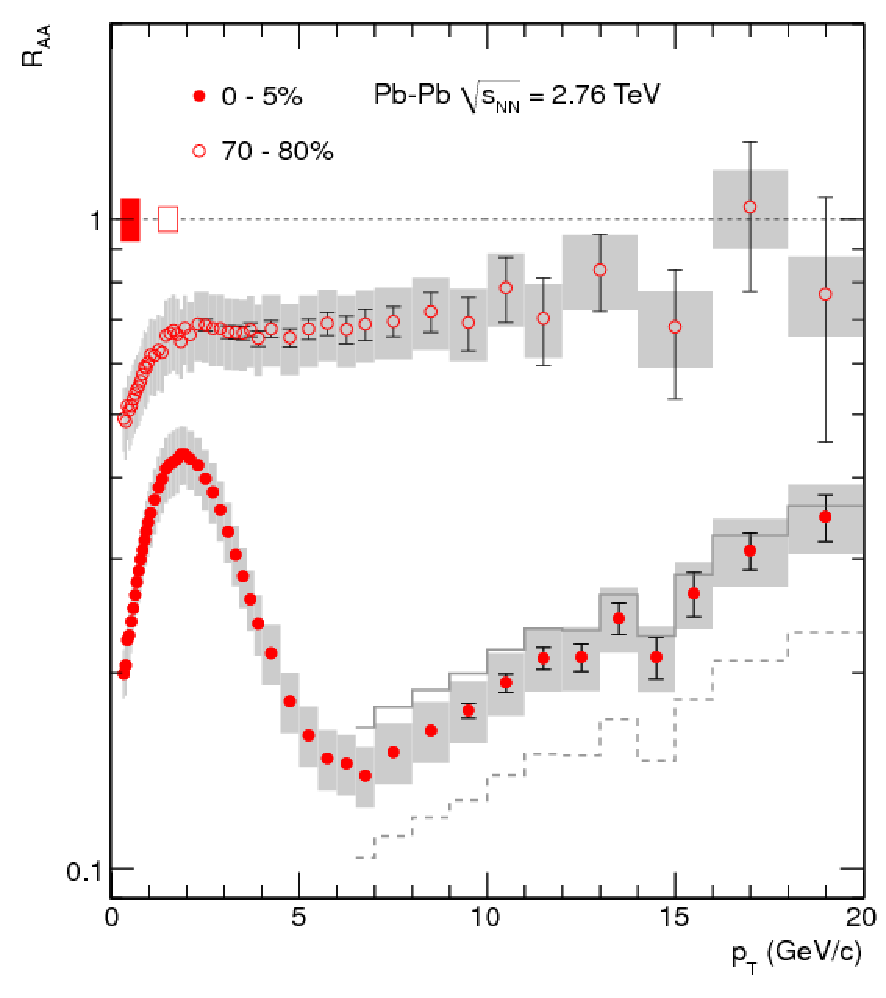
\includegraphics[width=0.85\linewidth]{images/Raa.pdf}
    \end{subfigure}%
    \begin{subfigure}{.5\textwidth}
        \centering
        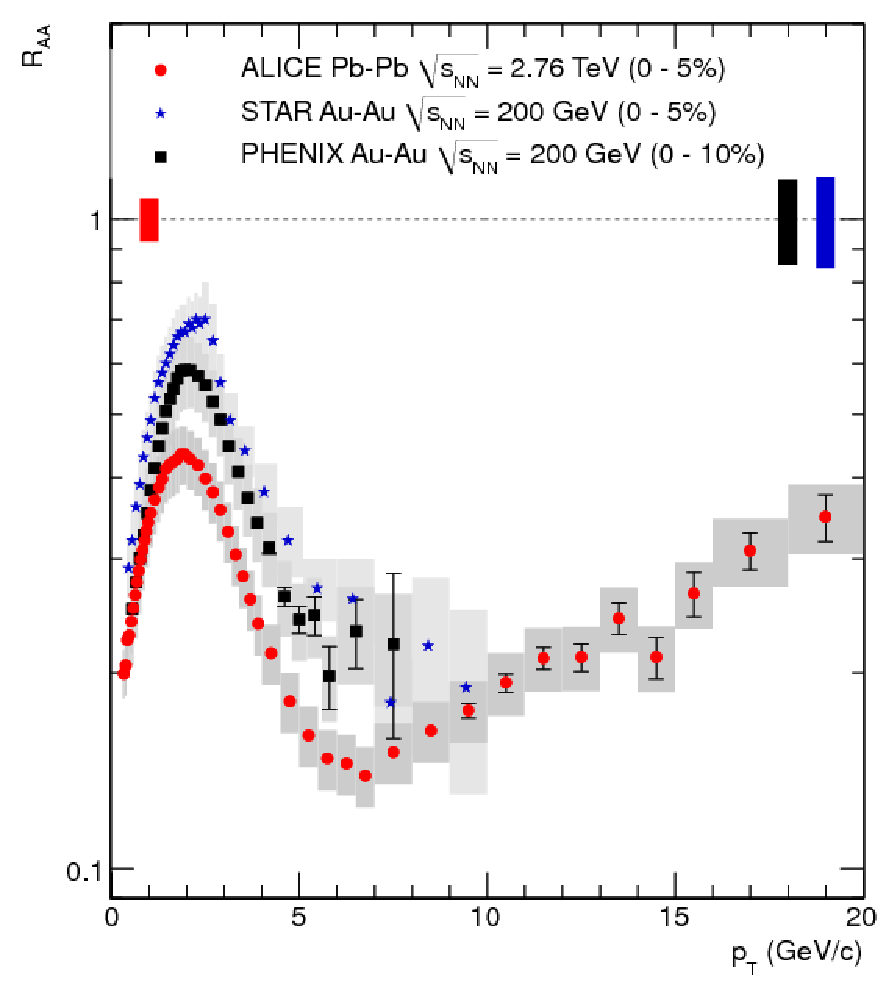
\includegraphics[width=0.85\linewidth]{images/CompRaa.pdf}
    \end{subfigure}
    \caption{Nuclear modification factor ($R_{\textnormal{\sc aa}}$) plots for central $(0-5\%)$ and peripheral $(70-80\%)$ Pb-Pb collisions at
        $\sqrt{s_{\textnormal{\sc nn}}} = 2.76$ TeV in ALICE (left). The central collision results are compared to Au-Au at $\sqrt{s_{\textnormal{\sc nn}}} = 200$
        GeV measurements from STAR and PHENIX (right)\cite{Raa:2010}.}
    \label{fig:raa}
\end{figure}

$R_{\textnormal{\sc aa}}$ measurements in p-Pb collisions at ALICE\cite{sami:2016} yield a value of unity consistent within systematic uncertainties across the
$p_{\textnormal{\sc t}}$ range, essentially disregarding any jet quenching and, therefore, QGP formation. Fig. \ref{fig:raappb} illustrates $R_{\textnormal{pPb}}$
measurements from ALICE at $\sqrt{s_{\textnormal{\sc nn}}} = 5.02$ TeV in blue beside $R_{\textnormal{PbPb}}$ results for central (red) and peripheral
collisions (green). It remains to be seen if Run 2 p-Pb collisions at higher energies $\sqrt{s_{\textnormal{\sc nn}}} = 8.16$ TeV conforms to these results.

\begin{figure}[H]
    \centering
    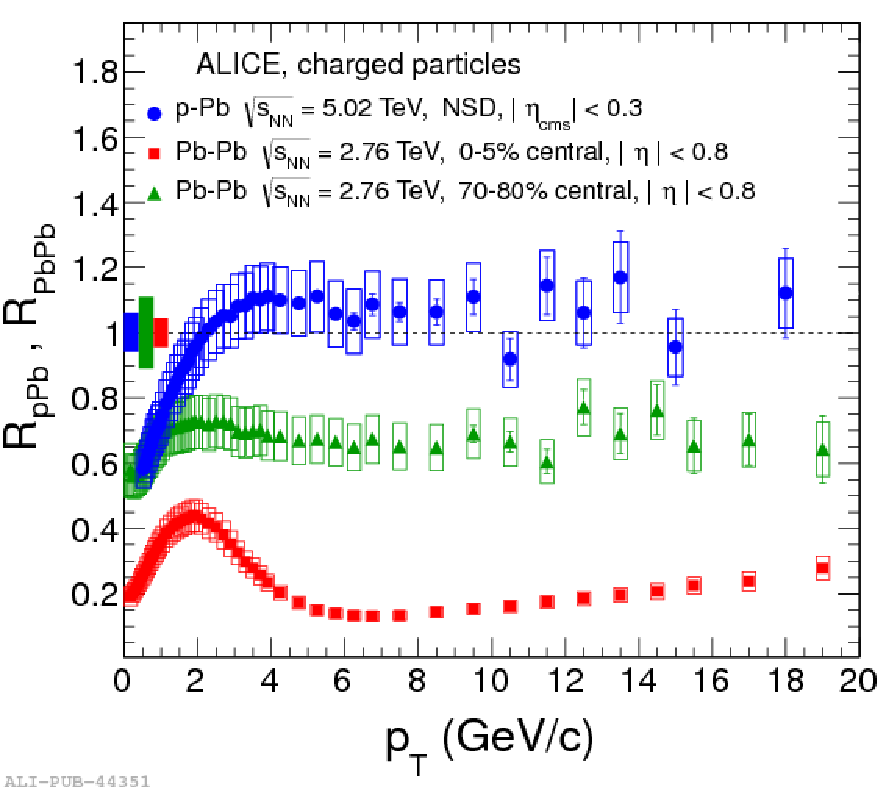
\includegraphics[width=0.7\linewidth]{images/Raappb.pdf}
    \\
    \caption{$R_{\textnormal{\sc aa}}$ for p-Pb collisions at $\sqrt{s_{\textnormal{\sc nn}}} = 5.02$ TeV (blue) compared with $\sqrt{s_{\textnormal{\sc nn}}}
            = 2.76$ TeV Pb-Pb central (red) and peripheral (green) collisions\cite{sami:2016}.}
    \label{fig:raappb}
\end{figure}

\subsection{Strangeness Enhancement}
One of the earliest suggested signatures for the formation of QGP was an increased yield of strange quark production in QGP as compared to a hadronic gas
phase in similar thermodynamic conditions.\cite{Muller:1982}. In the event of a deconfined phase of quarks and gluons (QGP), strange quark pairs production
($s\bar{s}$) can
be abundantly realised through gluon-gluon collisions ($gg \rightarrow s\bar{s}$) or light quark-antiquark annihilation ($q\bar{q} \rightarrow s\bar{s}$).
Strange quark pair production can even reach levels of saturation, i.e. the rate of $s\bar{s}$ annihilation matches its rate of formation, provided the
lifetime of the plasma is long enough. However, strange hadron production is much less abundant owing to a far higher energy threshold as compared to
strange quark pair production as hadron gases follow the hadronic degrees of freedom, rather than partonic. Therefore, strange hadron production
is touted as a signature for QGP formation, and can be observed by comparing strange hadron yields over pion yields in heavy-ion collisions to smaller
systems where QGP formation is not presumed, such as proton-proton and proton-ion collisions.

Earliest experimental indications for strangeness enhancement were observed for enhanced strange Kaon production at AGS, BNL\cite{AGS_Strangeness:1999}
and SPS, CERN\cite{Str_SPS1:1999,Str_SPS2:1999}. Strangeness enhancement was also measured for $\Lambda$\cite{Str_lambda:1989}, $\Xi$\cite{Str_Xi:1991},
and $\Omega\cite{Str_omega}$ particles at SPS. The strangeness content of a particle was predicted to be directly proportional to its expected enhancement.
Thus, the $\Omega$ baryon is expected to be the most enhanced due to this phenomenon, which was later experimentally confirmed\cite{Str_om2:1999}. This
was further verified at different energies and in different ion collision experiments, including LHC\cite{Str_LHC:2013}. Hyperon-to-pion ratios as a
function of average number of participating nucleons in a collision, $\langle N_{\textnormal{part}} \rangle$, measured at ALICE are depicted in Fig.
\ref{fig:hyp}.

\begin{figure}[H]
    \centering
    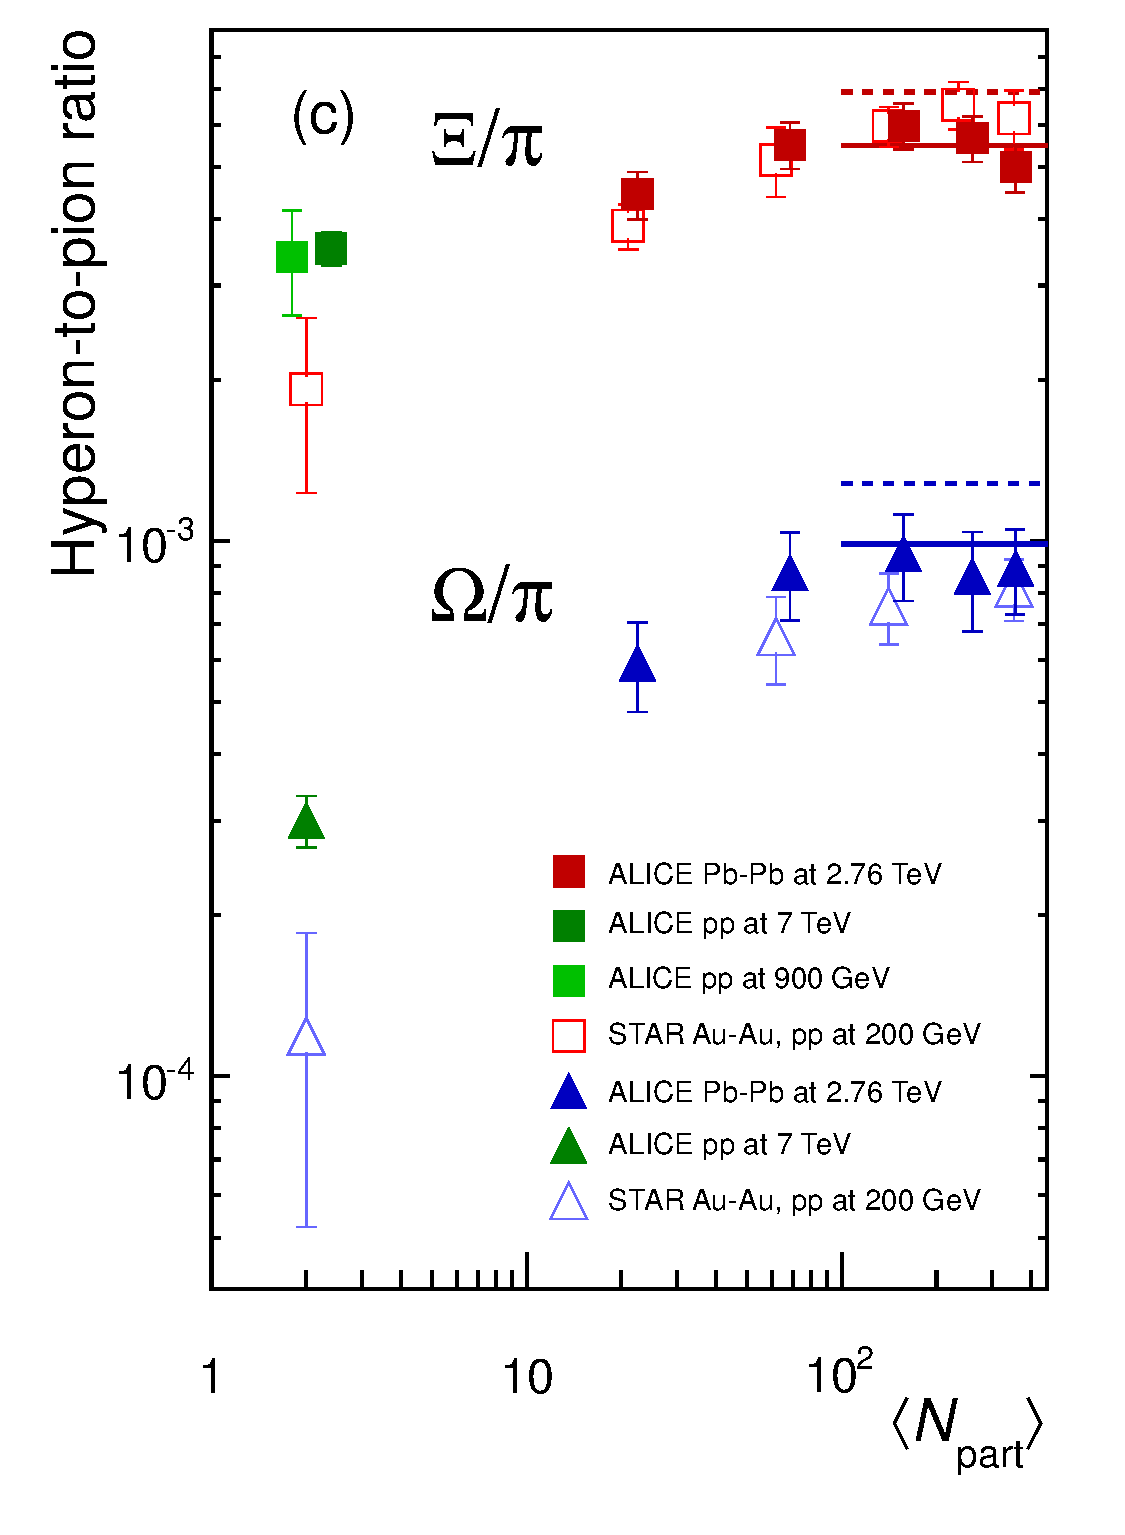
\includegraphics[width=0.5\linewidth]{images/hypToPion.pdf}
    \\
    \caption{Hyperon-to-pion ratios in Pb-Pb and p-p collisions as a function of $\langle N_{\textnormal{part}} \rangle$, ALICE. Results from STAR for
        comparison. Lines indicate thermal model predictions.\cite{Str_LHC:2013}}
    \label{fig:hyp}
\end{figure}

From the figure, the enhancement in Pb-Pb results is apparent as compared to p-p collisions. Results from STAR collaboration represented by open symbols
are plotted for comparison. The enhancement is comparatively weaker at LHC due to higher energy of p-p measurement taken as a reference.

Smaller systems such as proton-proton and proton-ion require a more detailed look, and instead of
$\langle N_{\textnormal{part}} \rangle$, the strange hadron yields were measured as a function of mean charged-particle multiplicity density
$\langle\textnormal{d}N_{\textnormal{ch}}/\textnormal{d}\eta\rangle$ (Fig. \ref{fig:had2pion}). Initial p-Pb measurements indicate a smooth increase in
hyperon-to-pion yields as a function of $\langle\textnormal{d}N_{\textnormal{ch}}/\textnormal{d}\eta\rangle$, nearly touching saturation levels as seen
in Pb-Pb data and projected by QGP thermodynamic models.


\begin{figure}[H]
    \centering
    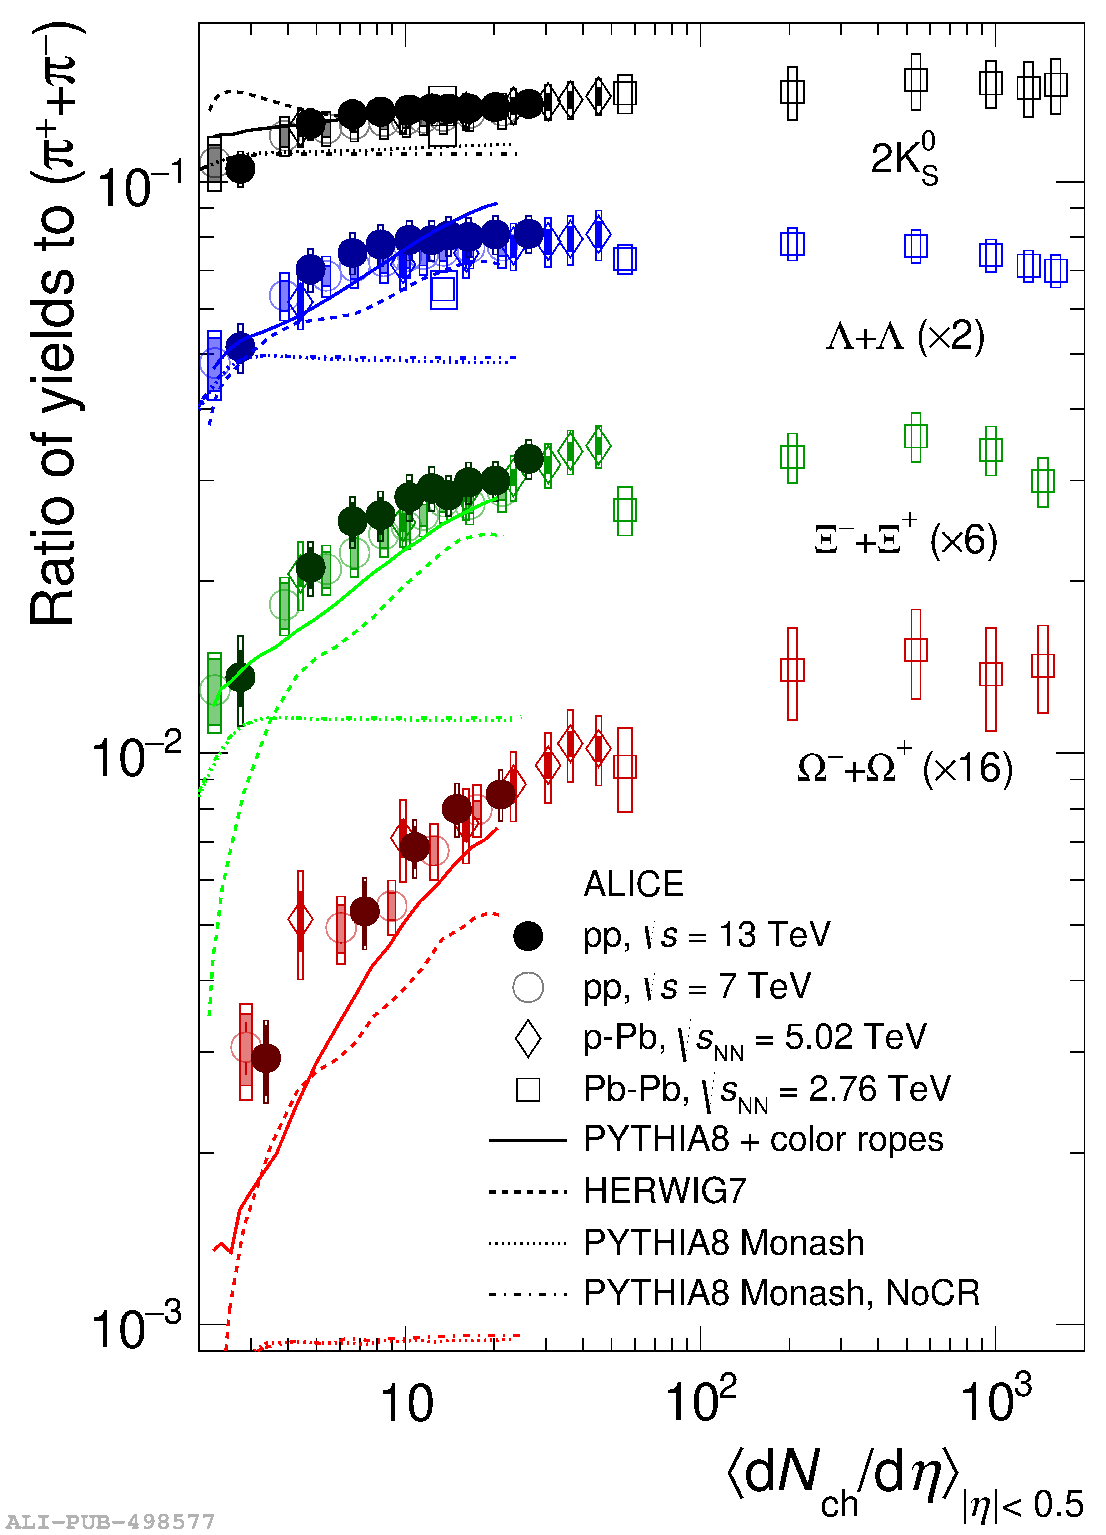
\includegraphics[width=0.5\linewidth]{images/HadronToPionRatio.pdf}
    \\
    \caption{Integrated strange hadron-to-pion ratios as a function of $\langle\textnormal{d}N_{\textnormal{ch}}/\textnormal{d}\eta\rangle$ in p-p, p-Pb
    and Pb-Pb collisions at ALICE\cite{Acharya:2020}.}
    \label{fig:had2pion}
\end{figure}

As is the case with p-Pb, a similar trend can be observed in p-p results with yield ratios steadily increasing as a function of multiplicity, seemingly
independent of collision system. The trend is best described by PYTHIA8 + color ropes approach, with other models varying in accuracy.

Baryon-to-meson ratios must also be evaluated for both strange and non-strange particles to rule out the possibility that the observed results are a mass
effect. $\Lambda/K_{\textnormal{\sc s}^{0}}$ and $p/\pi$ ratios are plotted in Fig. \ref{fig:bar2meson} to determine if there is any multiplicity dependence.
From the figure, it can be seen that the ratio curves are almost flat and no multiplicity dependence is observed, confirming that the enhancement is not
related to differences in hadron mass.

\begin{figure}[H]
    \centering
    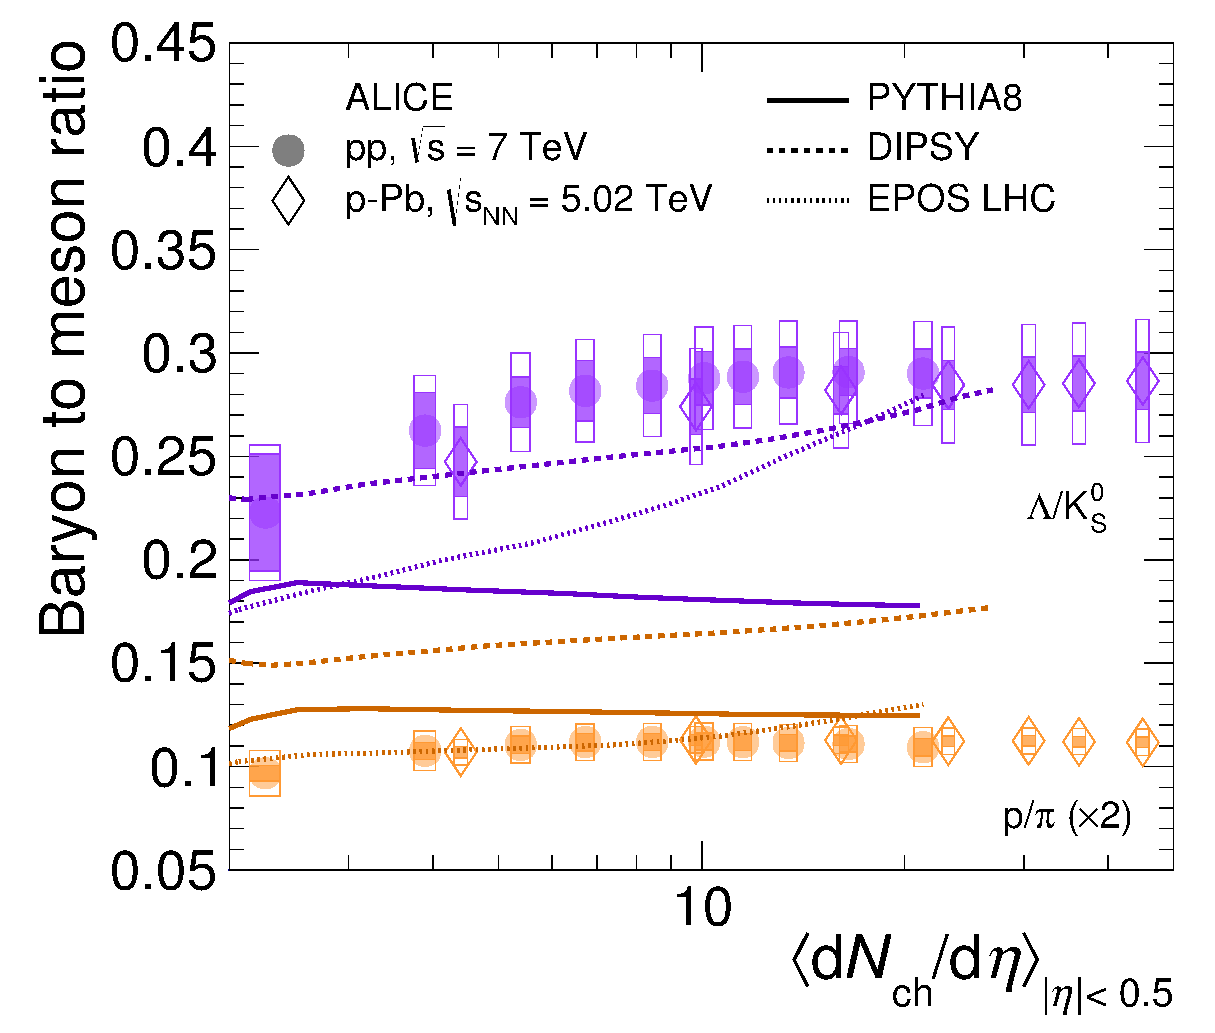
\includegraphics[width=0.7\linewidth]{images/bmratio.eps}
    \\
    \caption{Particle yield ratios $\Lambda/K^{0}_{\textnormal{\sc s}}$ and $p/\pi$ as a function of
    $\langle\textnormal{d}N_{\textnormal{ch}}/\textnormal{d}\eta\rangle$, ALICE\cite{nature:2016}.}
    \label{fig:bar2meson}
\end{figure}
\chapter{Goals of the Dissertation thesis}
\begin{itemize}
    \item In-depth familiarisation with the ALICE software environment, the ROOT data analysis framework, AliRoot software framework and libraries, 
          AliPhysics classes and the Worldwide LHC Computing GRID infrastructure.
    \item Selection criteria optimization for reconstruction of multi-strange cascade candidates ($\Xi^{\pm}, \Omega^{\pm}$).
    \item Raw (uncorrected) transverse momentum extraction for cascade particles in p-Pb collisions at $\sqrt{s_{NN}}$ = 8.16TeV distributed over 
          different multiplicity classes.
    \item Detector efficiency estimation and acceptance correction using Monte Carlo simulations. 
    \item Applying efficiency corrections to obtain corrected transverse momentum spectra for different multiplicity classes.
    \item Analysis of the mean transverse momenta, integrated yields, and adjusted $p_{\textnormal{T}}$ spectra for systematic errors and uncertainities.
\end{itemize}
\chapter{Overview of the experimental setup}
\section{Experiments at LHC}
The Large Hadron Collider (LHC), presently the largest and most powerful particle accelerator in the world, is home to a number of particle physics
experiments involving the Standard Model, dark matter, matter-antimatter ratio and Quark-Gluon Plasma, among others. Located in a 27 km long tunnel
about 100 m underground along the Franco-Swiss border, the accelerator was commisioned in 2008 by the European Organization for Nuclear Research
(CERN), a collaboration of thousands of scientists, researchers, engineers and students all over the world. The LHC is the latest addition to the
CERN accelerator complex, serving a diverse array of experiments.

The Accelerator Complex at CERN (Fig. \ref{fig:Cern-accelerator-complex}) is a collection of particle accelerators that work in tandem to boost the
energy of a beam of particles in order to accelerate them close to the speed of light. This is achieved through several accelerators in sequence,
with LHC being the final accelerator currently boasting energies up to 6.5 TeV per beam.

\begin{figure}[H]
    \centering
    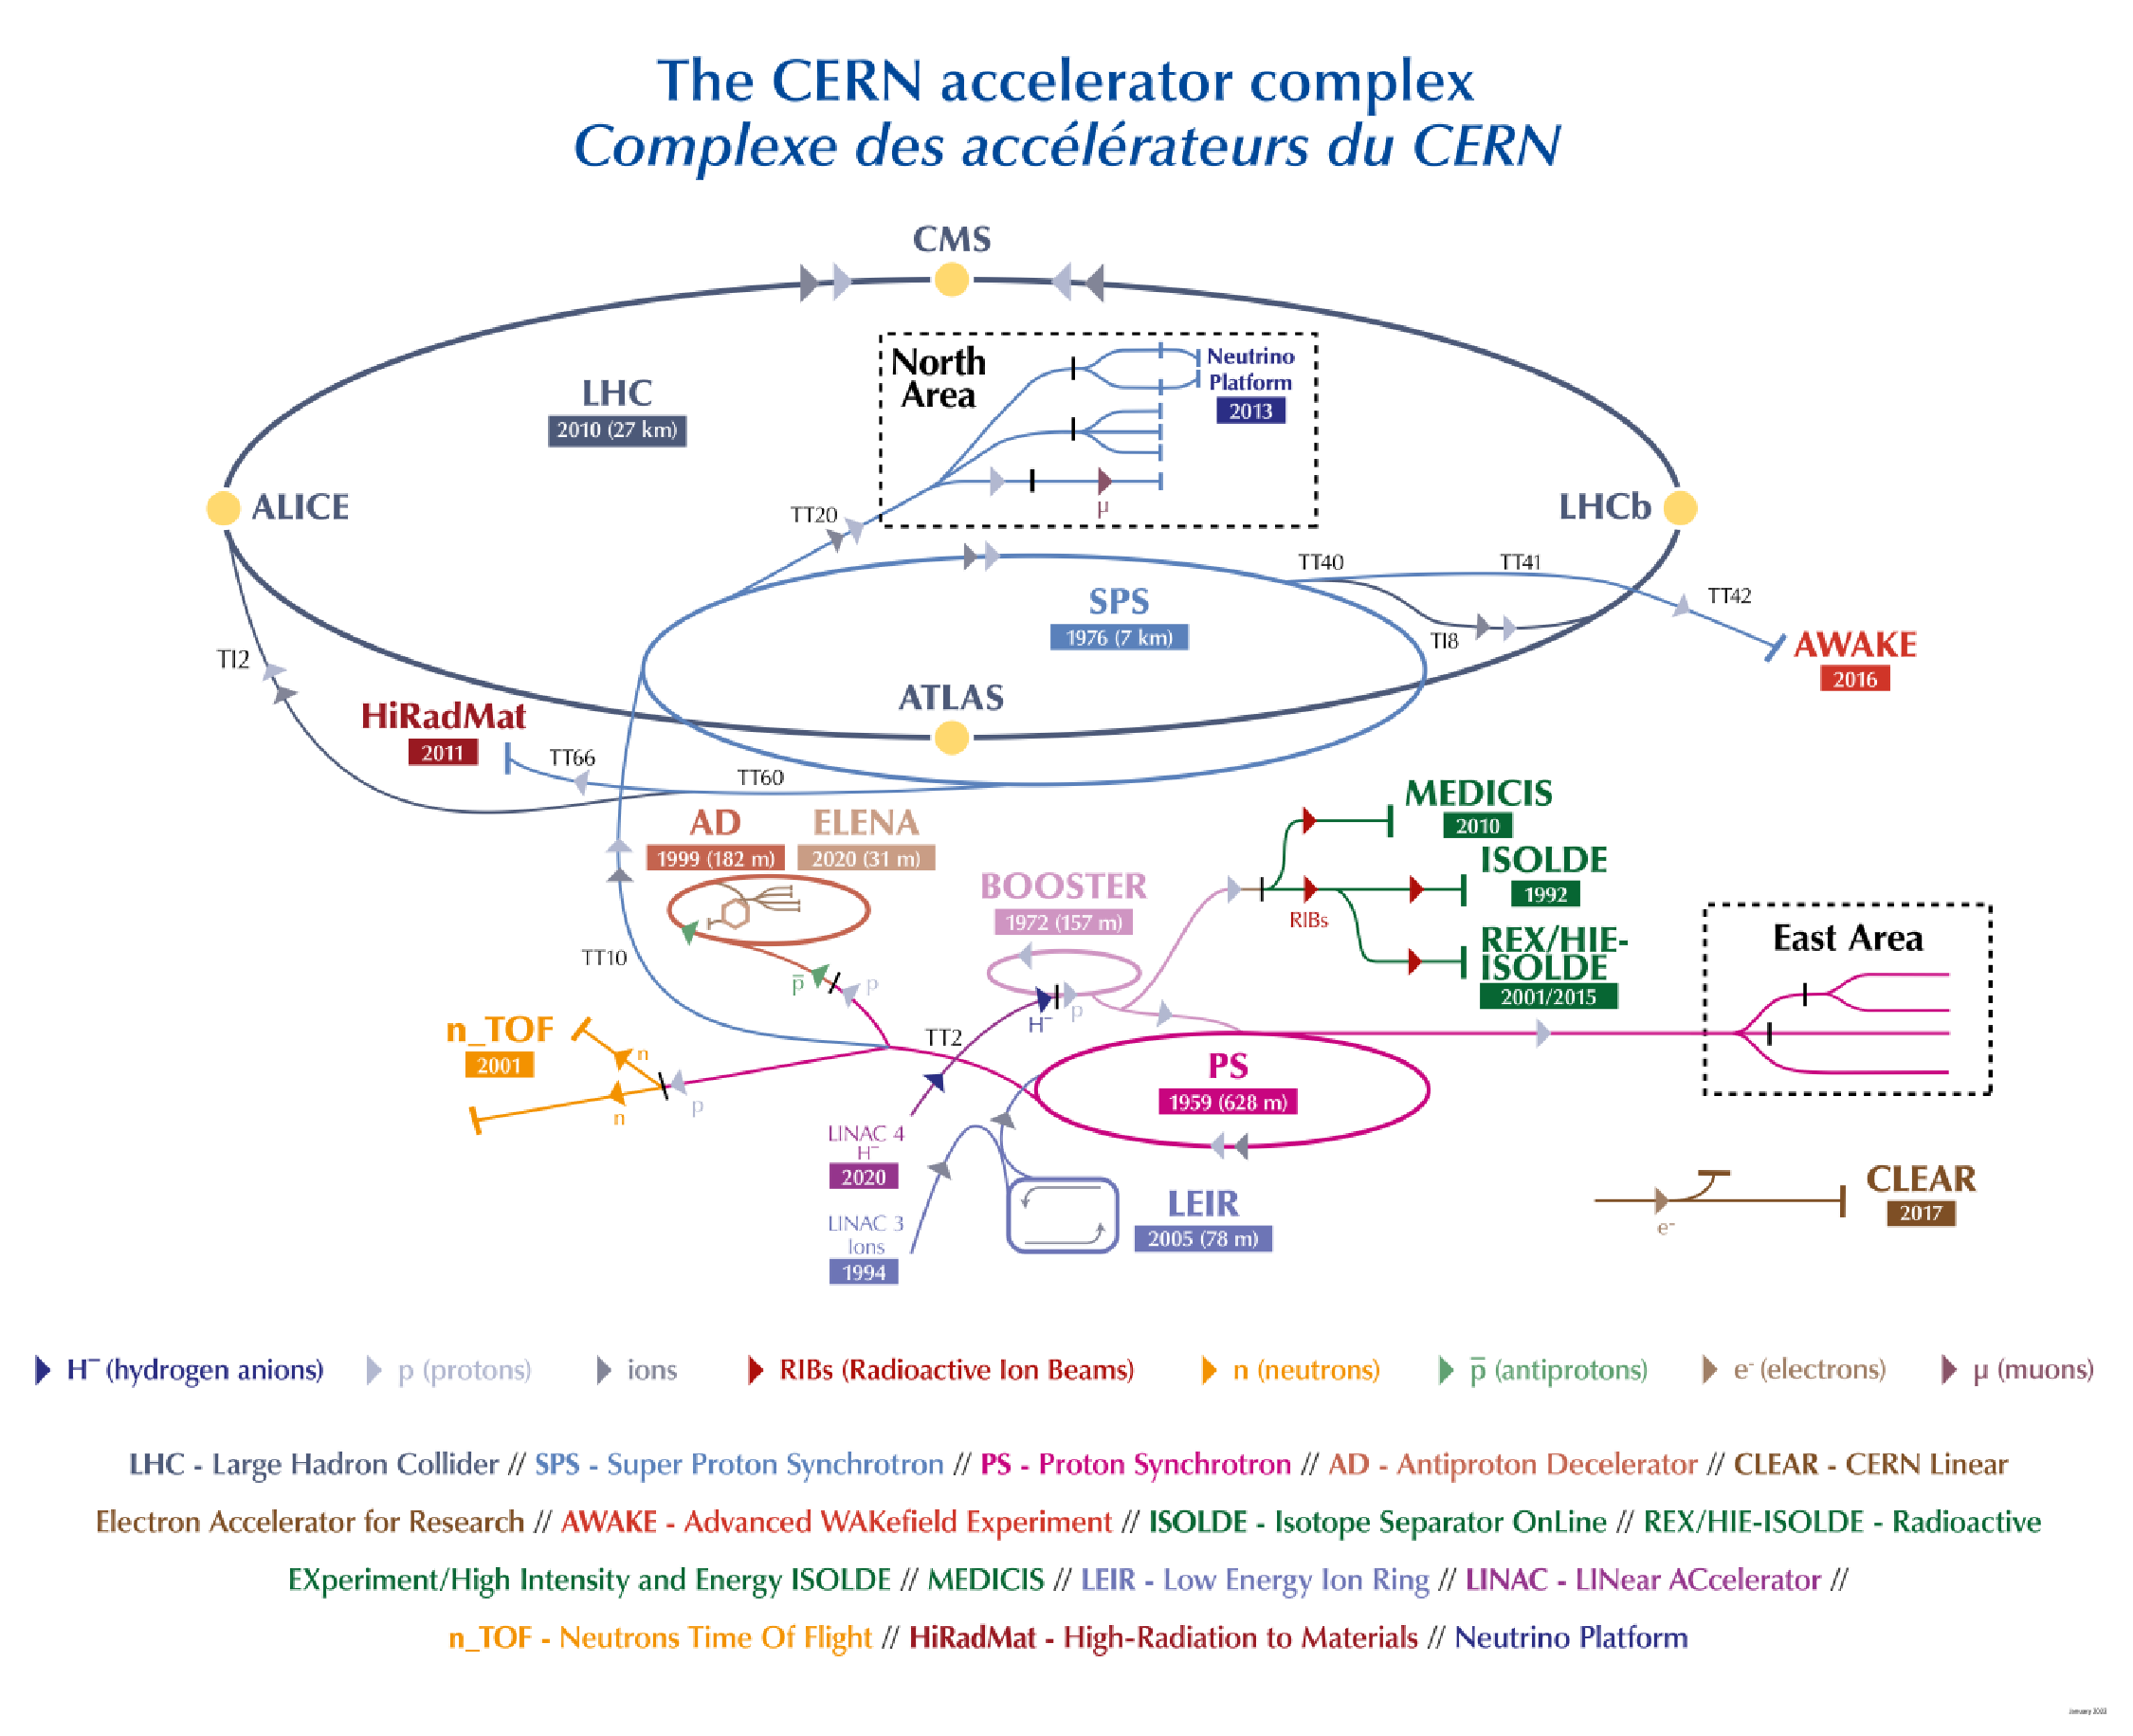
\includegraphics[width=\linewidth]{images/acceleratorComplex.pdf}
    \\
    \caption{CERN Accelerator Complex\cite{acceleratorComplex:2022}}
    \label{fig:Cern-accelerator-complex}
\end{figure}

Particle collisions in the LHC are used in several experiments to study diverse phenomena:

\begin{itemize}
    \item Testing the parameters of the Standard Model and the study of rare particles, such as the Higgs boson (discovered at LHC in 2012).
    \item Probing into particles or phenomena that account for dark matter and dark energy.
    \item The predominance of matter over antimatter in the Universe.
    \item To study and find evidence for supersymmetry.
    \item Recreating conditions akin to those just after the Big Bang, in search of the Quark-Gluon Plasma phase to study the generation of particles
          that constitute matter.
\end{itemize}

Particle acceleration in the LHC's circular particle synchrotron design is achieved through acceleration and bending the beamline across its 27 km
long circumference with an array of superconducting magnets cooled down to temperatures in the vicinity of 1.9 K by the use of liquid Helium. Two
simultaneous anti-parallel proton or ion beams, made up of particle 'bunches', are accelerated up to appropriate energies and circulated while collisions
occur at four chosen intersection points. The collisions can amount to as much as 13 TeV centre-of-mass energy and peak luminosity values of
$2\times10^{34}cm^{-2}s^{-1}$\cite{LhcReport:2018}. These collisions are studied by several experimental stations situated throughout the beamline.
Four main experiments in the LHC complex, employing massive detector assemblies, include:

\begin{itemize}
    \item ATLAS (A Toroidal LHC Apparatus)
    \item CMS (Compact Muon Solenoid)
    \item LHCb (LHC-beauty)
    \item ALICE (A Large Ion Collider Experiment)
\end{itemize}

The ATLAS and CMS are the two main general purpose detectors covering a broad area of physics including, but not limited to, Standard Model and theories
extending beyond SM like supersymmetry, the search for Higgs boson and its properties and search for particles that could constitute dark matter. The
LHCb and the ALICE experiments are dedicated to more specialised purposes. LHCb focuses on b-quark physics to detect minute differences in matter and
antimatter, aiming to find CP violation in b-hadron interactions. The ALICE experiment is designed to scrutinise the signatures for the formation of
Quark-Gluon Plasma and observe particle creation pertaining to QGP's subsequent hadronisation.

\section{The ALICE Detector}
The ALICE detector (Fig. \ref{fig:ALICEdetector}) is a 10,000 tonne machine located at interaction point 2 in the LHC complex, optimised for studying heavy ion collisions and
reconstructing particle tracks using subdetector modules at high particle densities. The main objectives for the ALICE experiment include studying
strongly interacting matter at high energy densities. The subdetectors allow comprehensive data collection of particle parameters for hadrons,
electrons, muons and photons produced in heavy-ion, lighter nuclei as well as proton-nuclear collisions at varying energy densities and multiplicity
ranges. The data presented in this report is based on p-Pb collisions at centre-of-mass energy of 8.16 TeV observed at the ALICE detector.


\begin{figure}[H]
    \centering
    \includegraphics[width=0.9\linewidth]{images/aliceRun2.eps}
    \caption{A schematic of the ALICE detector (Run 2)\cite{Tauro:2017}}
    \label{fig:ALICEdetector}
\end{figure}

At 26 m long, 16 m high and 16 m wide, the ALICE detector sits concentrically around the beam axis. Boasting a full 2$\pi$ azimuthal coverage around
the beamline, the $\eta$ coverage is dependent on each detector component though, as is shown in Fig. \ref{fig:etaAcceptance}.

\begin{figure}[H]
    \centering
    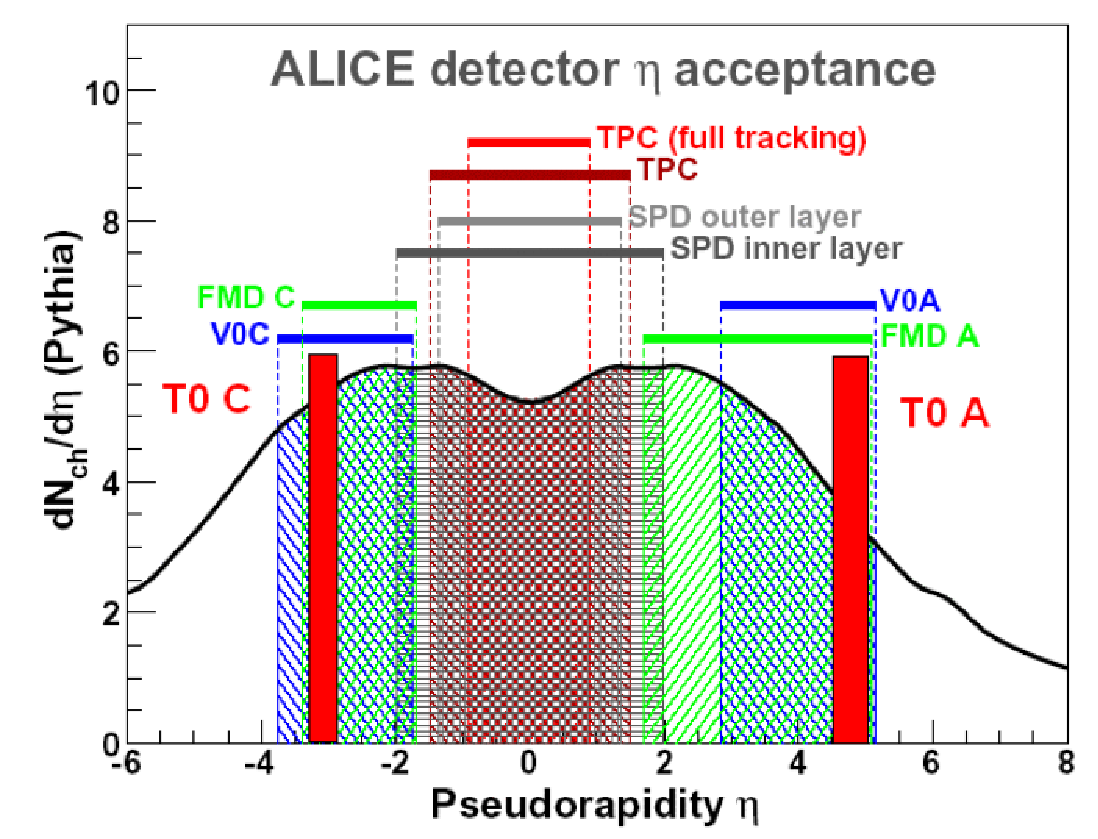
\includegraphics[width=0.7\linewidth]{images/etaAcceptance.pdf}
    \caption{$\eta$ acceptance for each subdetector in ALICE\cite{Nayak:2009}}
    \label{fig:etaAcceptance}
\end{figure}

The ALICE global coordinate system is used as reference to describe parameters of reconstructed tracks as well as detector positions. A right-handed
Cartesian coordinate system with origin at nominal interaction point is assumed, with the $z$-axis along the beam direction. The $x$ and $y$ axes are
horizontal and vertical respectively -- with positive $x$ pointing towards centre of LHC ring and positive $y$ pointing upwards. Each of the 19
subdetectors, part of the ALICE detector complex in LHC's Run 2 phase, measures certain observables which, when combined together, shed
light on the whole picture of the collision. Three major sections make up the detector complex:
\begin{itemize}
    \item The central part
    \item The muon detector
    \item The small angle detectors
\end{itemize}

The central part, spanning the polar angles from 45\degree{} to 135\degree{}, can detect hadrons, photons and electrons. The beam interaction takes place
in the central part, made up of several detectors in the order starting from the geometric centre:
\begin{enumerate}
    \item Inner Tracking System (ITS), which consists of$\colon$
          \begin{itemize}
              \item The Silicon Pixel Detector (SPD)
              \item The Silicon Drift Detector (SDD)
              \item The Silicon Strip Detector (SSD)
          \end{itemize}
    \item Time-Projection Chamber (TPC)
    \item Time-of-Flight (TOF) Chamber
    \item Transition Radiation Detector (TRD)
    \item Photon Spectrometer (PHOS)
    \item Electromagnetic Calorimeter (EMCal)
    \item High Momentum Particle Indentification (HMPID)
\end{enumerate}

ITS and TPC, which are used in tracking the particles, measure particle position and particle trajectory evolution, enabling particle track reconstruction
in 3D space. All of the above subdetectors cover the entire 2$\pi$ azimuthal range, except HMPID, PHOS and EMCal.
The muon detector chamber, covering an angle from 2\degree{} to 9\degree{}, is made up of several absorbers, a large dipole magnet, and ten detection planes
used in path determination from the trigger chamber's four planes. The small angle detectors help to determine global characteristics and trigger signals.
Initial state of collisions and the collision strength is deduced by measuring remnants of the colliding particles with the help of$\colon$
\begin{enumerate}
    \item Forward Multiplicity Detector (FMD)
    \item Photon Multiplicity Detector (PMD)
    \item Zero Degree Calorimeter (ZDC)
    \item Small angle detector (V0)
    \item Fast timing and trigger detector (T0)
\end{enumerate}

ZDC measures the spectator nucleons' energy, while FMD and V0 measure distribution and multiplicity of daughter particles. The T0 detects determines
time of collision. In regards to the scope of this work, the detectors holding relevant significance for analysis of strange particles are detailed as
follows$\colon$

\subsection{The ALICE VZERO System}
The ALICE VZERO System\cite{vzero:2013}, comprising of two scintillator arrays (VZERO-A and VZERO-C) on each side of interaction point, plays a crucial role as the
lowest level trigger (L0) source. It also monitors LHC beam conditions, luminosity, azimuthal distribution, particle multiplicity and is used for
rejecting beam-induced background.

\begin{figure}[H]
    \centering
    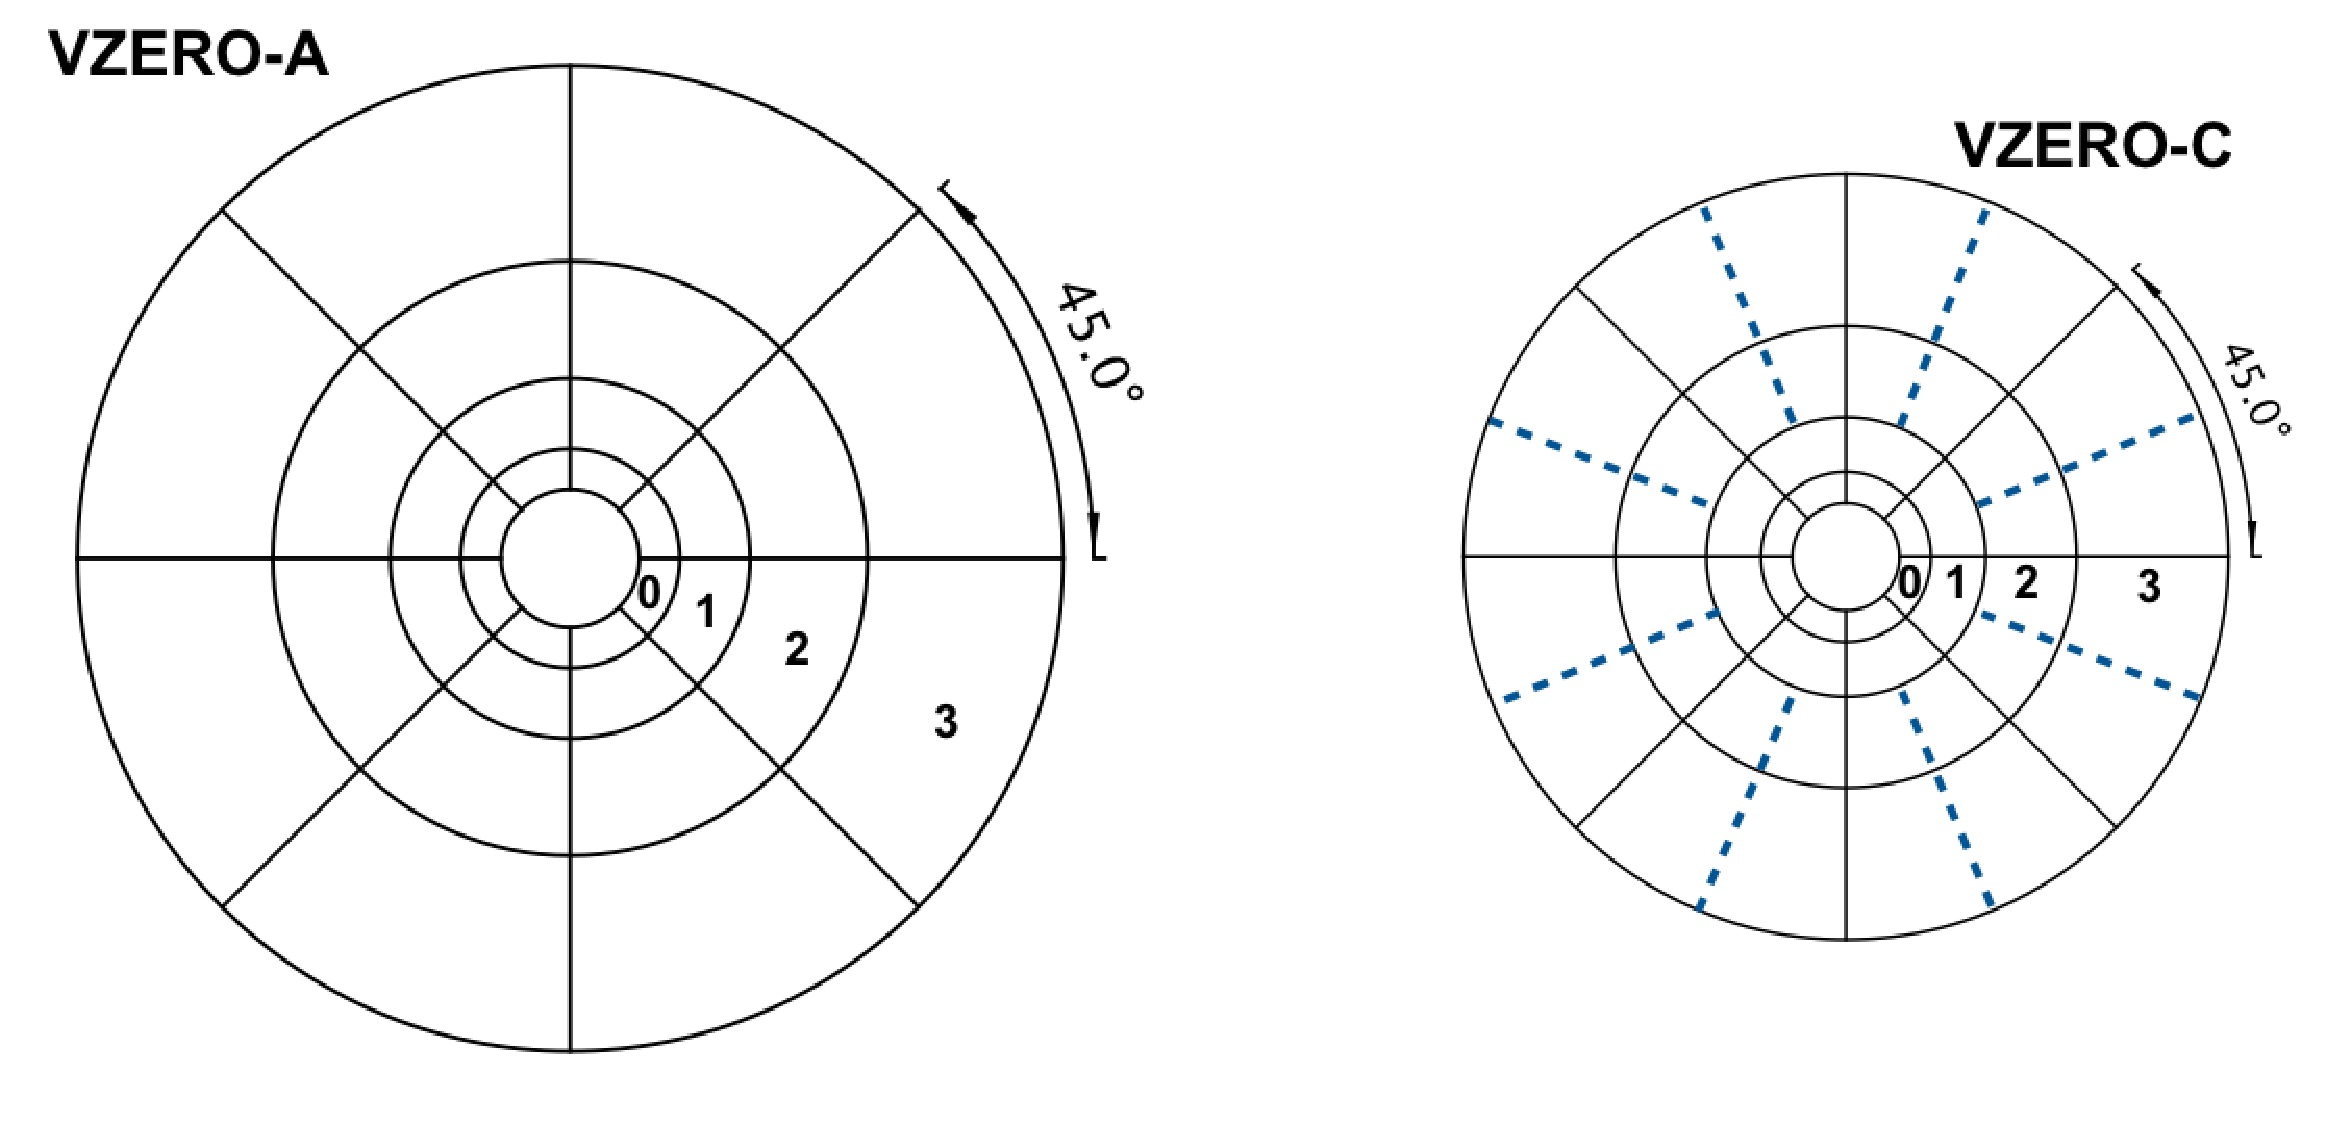
\includegraphics[width=0.7\linewidth]{images/vzero.eps}
    \caption{VZERO-A and VZERO-C segmentation\cite{vzero:2013}}
    \label{fig:vzero}
\end{figure}

The pseudorapidity ranges $2.8 < \eta < 5.1$ and $-3.7 < \eta < -1.7$ (Fig. \ref{fig:etaAcceptance}) are covered by VZERO-A and VZERO-C respectively.
With a radius of 41.2 cm, the VZERO-A is located opposite to the muon spectrometer, 329 cm from the nominal vertex ($z=0$). On the other hand, VZERO-C
is located 86 to 88 cm from the nominal vertex, with a radius of 32 cm. Each VZERO array is radially segmented into four rings, where each ring is an
subdivided into eight azimuthal sections (Fig. \ref{fig:vzero}).

The energy deposited in the scintillators enable charged particle multiplicity measurements in the VZERO system. Additionally, owing to the granularity
in the azimuthal direction, the VZERO system also helps in reaction plane estimation.

\subsection{Inner Tracking System}

The ALICE Inner Tracking System (ITS), owing to its proximity to the interaction region, is the principal detector resposible for determining the
primary interaction vertex. It plays a crucial role to measure the precise location of particles, especially in the study of short-lived hadrons
to identify secondary vertices and their decay patterns through vertex reconstruction. Composed of six cylindrical silicon semiconductor layers whose
distance from the beam line varies from 3.9 cm to 43 cm for the outermost layer, the ITS spans the central pseudo-rapidity range of $|{\eta}| < 0.9$\cite{ITS:2015}.

\begin{figure}[H]
    \centering
    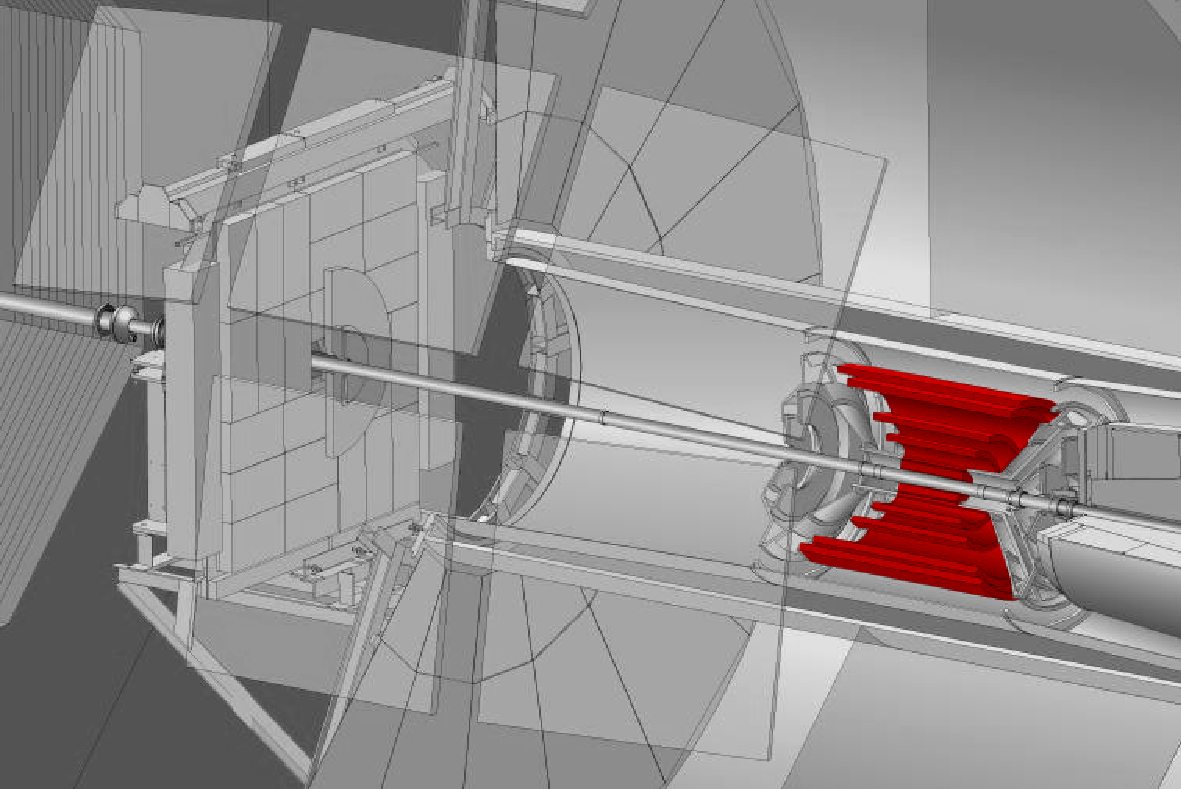
\includegraphics[width=0.7\linewidth]{images/its.pdf}
    \caption{ITS' position and concentric barrel design in ALICE Run 2\cite{Schematics:2017}}
    \label{fig:its}
\end{figure}

The six layers of ITS employ three different detector technologies. The two innermost layers are made of hybrid pixels, called the Silicon Pixel
Detector (SPD). The next two layers constitute the Silicon Drift Detector (SDD), and the two outermost layers important for track matching to the TPC
are the Silicon Strip Detector (SSD). Some of the ITS' capabilities are$\colon$
\begin{itemize}
    \item Primary vertex location with a resolution of $10^{-4}$ m.
    \item Secondary vertex reconstruction from hyperon and D and B meson decay.
    \item Tracking and identification of particles with momentum < 100 MeV.
    \item Momentum and angle resolution improvements for high $p_{\textnormal{T}}$ particles traversing through the TPC.
    \item Reconstruction (albeit with limited momentum resolution) of paths of particles passing through TPC's dead regions
\end{itemize}

Owing to its diverse use cases and a pivotal position in tracking measurements, ITS' significance can be easily realised in most experiments.

\subsection{Time Projection Chamber}

The Time Projection Chamber (TPC) is the main particle identification and tracking detector in the ALICE experiment. TPC's strengths include charged
particle reconstruction in three spatial dimensions, and in conjunction with other central barrel detectors, momentum measurements with a focus on
two-track separation, particle identification and vertex determination. Covering the full azimuth range and central pseudo-rapidity range of
$|{\eta}| < 0.9$ for tracks crossing the whole detector, the acceptance increases to $|{\eta}| < 1.5$ for larger pseudo rapidities with shorter TPC
track length ($\frac{1}{3}$ of radial track length).

\begin{figure}[H]
    \centering
    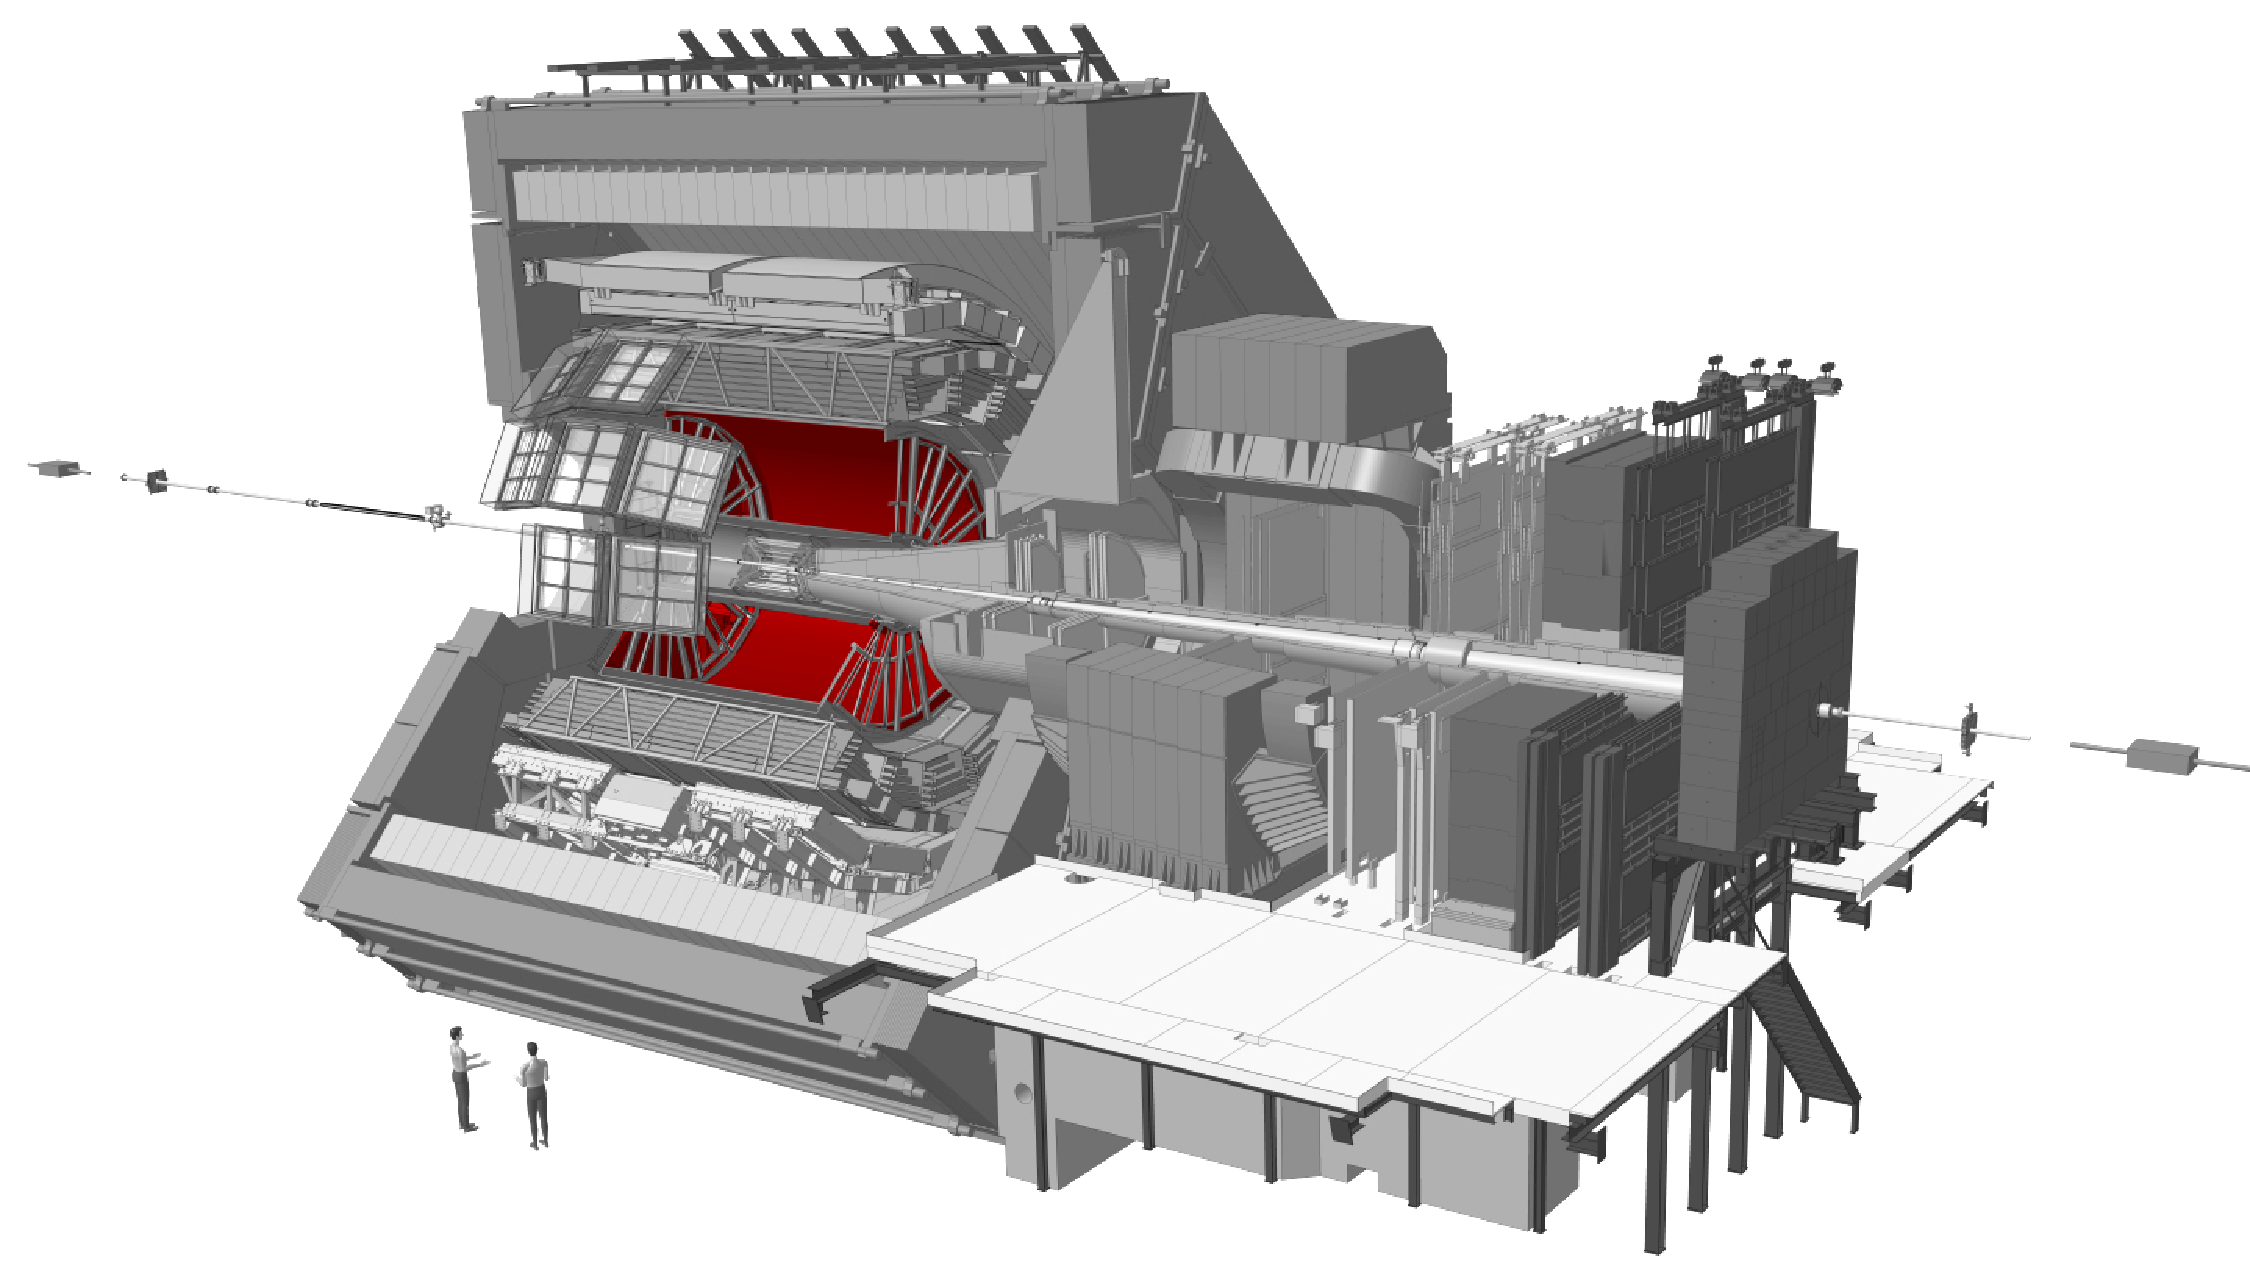
\includegraphics[width=0.8\linewidth]{images/tpc.pdf}
    \caption{Layout of TPC's position in the ALICE detector\cite{Schematics:2017}}
    \label{fig:tpc}
\end{figure}

Cylindrical in shape with an inner radius of 848 mm and an outer radius of 2466 mm, the TPC is filled with 88 m$^{3}$ of gaseous mixture of Ne-CO$_{2}$-N$_{2}$
as a counting gas, with the total length of 4.994 m of the hollow cylinder segregated into drift regions by the central high voltage electrode situated
at $z = 0$. A drift field of 400 V/cm is generated pointing towards the central electrode, which is kept at a drift voltage of -100kV.

Upon encountering charged particles, the TPC gas is ionized creating ions and free electrons, which are then separated in the drift field. The electrons
drift towards the end plates which are supplied with 36 readout chambers each, organized in 18 sectors covering 20\degree{} in azimuth individually.
The ions drift about a 1000 times slower than the electrons. The two dimensional position reconstruction is achieved through the signal induced due to
movement of electrons on the pad plane. The signal magnitude can be used to determine the strength of ionisation, and therefore the energy loss
($\frac{-\textnormal{d}E}{\textnormal{d}x}$). The drift time of the electrons is used to reconstruct the third spatial dimension ($z$ coordinate).

The TPC is utilized to register the following observables$\colon$
\begin{itemize}
    \item Momentum resolution
    \item $dE/dx$ resolution
    \item Azimuthal coverage
    \item Track matching
    \item Two-track resolution
\end{itemize}

\subsection{Time-of-Flight Detector}

The Time-of-Flight (TOF) detector, with the support of TPC, is used for identifying charged particles by determining their mass. This is accomplished 
by timing the passage of a particle track from the initial interaction vertex to the point at which a hit is registered in the TOF detector. In 
conjunction with the tracking detectors' measurements of momentum and trajectory length, the particle's mass can be calculated. The TOF's 
upper hand in particle identification is especially realised in the momentum ranges where TPC's ($\frac{-\textnormal{d}E}{\textnormal{d}x}$) cannot 
be used. 

\begin{figure}[H]
    \centering
    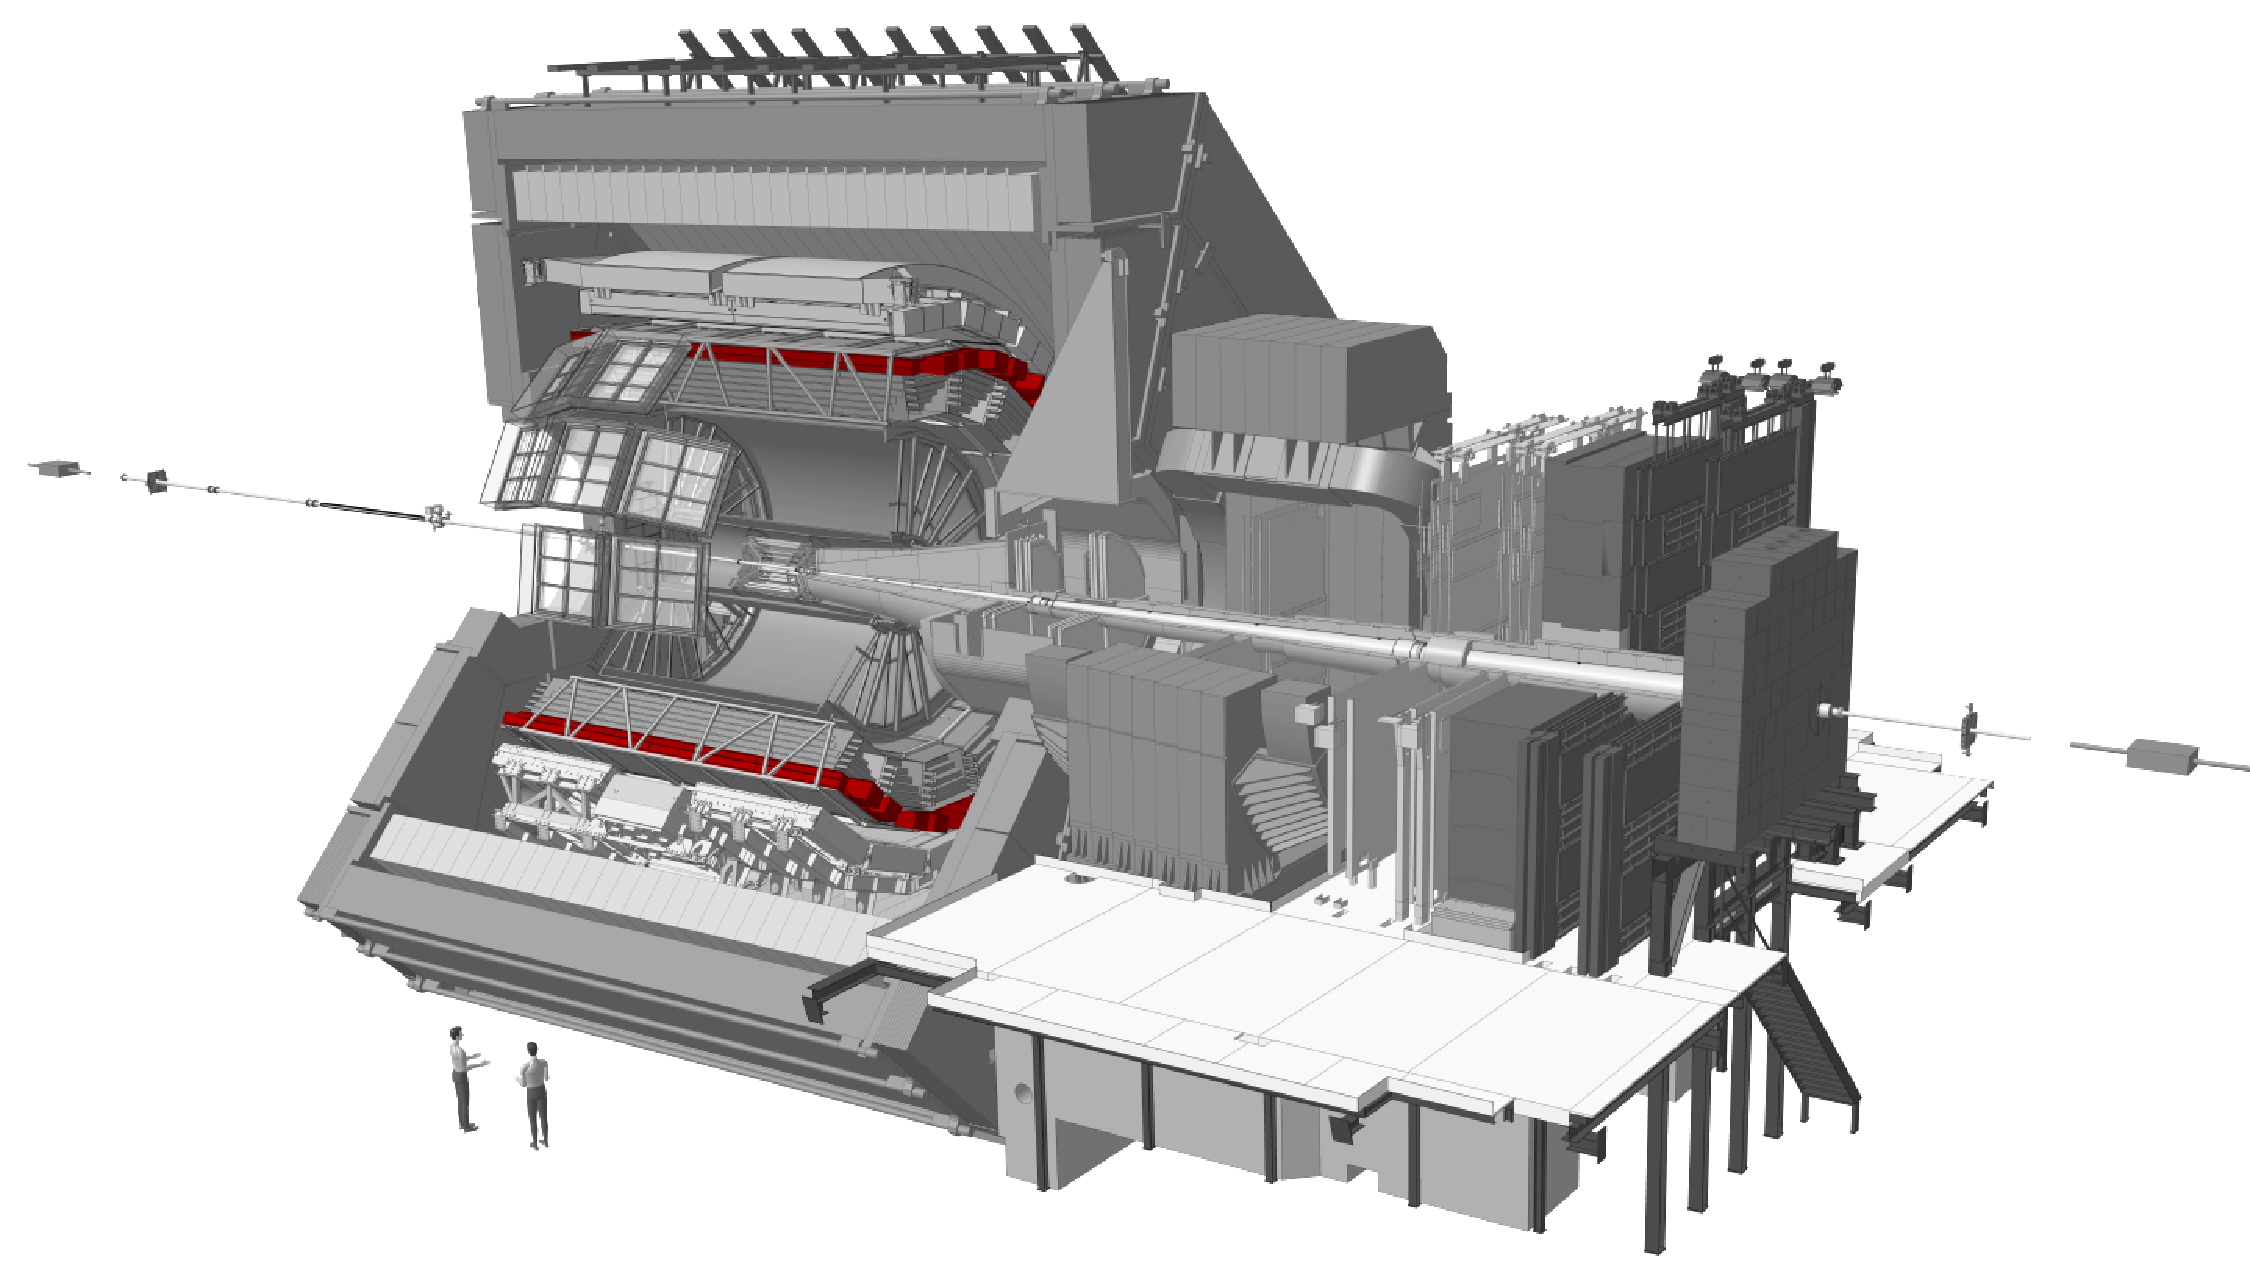
\includegraphics[width=0.8\linewidth]{images/tof.pdf}
    \caption{Layout of TOF's position in the ALICE detector\cite{Schematics:2017}}
    \label{fig:tof}
\end{figure}

Similar to the TPC, TOF also follows a hollow cylinder design with full azimuthal coverage and $|{\eta}| < 0.9$. With an outer radius of 3.78 m, it 
imitating the 18-fold segmentation of the TPC (and TRD). 
Specifically, at the $3\sigma$ level, TOF offers proton/kaon separation up to 2.5 GeV/$c$ and pion/kaon separation up to 4 GeV/$c$. Additionally, TOF 
data is also used to enhance the identification of electrons and nuclei.


\chapter{Analysis Details}

\section{Multi-strange baryons}
Multi-strange baryons, possessing more than one strange quark, are of particular importance in the study of particle production mechanisms, as their dominant
strange quark content makes them susceptible to changes in hadrochemistry of the colliding systems. This analysis attempts to probe the multi-strange
baryon yields in proton-lead (p-Pb) collisions at centre-of-mass energy of $\sqrt{s_{\textnormal{\sc nn}}}$ = 8.16 TeV measured at the ALICE detector in
LHC. A total of six multi-strange baryons, including $\Xi^{0} (uss)$, $\Xi^{-} (dss)$, and $\Omega^{-} (sss)$, along with their corresponding antiparticles
$\bar{\Xi^{0}}$, $\bar{\Xi^{+}}$, and $\bar{\Omega^{+}}$ are of interest. They are known as cascade particles owing to their doubly weak decay mechanism.
Since the initial state colliding particles do not contain any strange valence quarks, all particles with a non-zero strangeness quantum number are
generated during the course of the collision. A summary of particles of interest along with their decay paths and branching ratios are tabulated in
Table \ref{tab:cascades}.

\begin{table}[H]
    \centering
    \begin{tabular}{|l|r|l|r|r|}
        \hline
        Particle                  & Mass (MeV/$c^{2}$)   & Decay Mode          & Branching Ratio (\%) & Lifetime $c\tau$ (cm) \\ \hline
        $\Xi^{0}$                 & $1314.86 \pm 0.20$   & $\Lambda \pi^{0}$   & $99.525 \pm 0.012$   & 8.71                  \\ \hline
        $\Xi^{\pm}$               & $1321.71 \pm 0.0.07$ & $\Lambda \pi^{\pm}$ & $99.887 \pm 0.035$   & 4.91                  \\ \hline
        $\Omega^{\pm}$            & $1672.45 \pm 0.29$   & $\Lambda K^{\pm}$   & $67.8 \pm 0.7$       & 2.461                 \\ \hline
        $\Lambda / \bar{\Lambda}$ & $1115.683 \pm 0.006$ & $p^{\pm} \pi^{\mp}$ & $63.9 \pm 0.05$      & 7.89                  \\ \hline
    \end{tabular}
    \caption{Cascade baryons and their properties\cite{Pdg:2018}}
    \label{tab:cascades}
\end{table}


The inner tracking detectors of the experimental setup in ALICE are capable of identifying only charged particles, and thus $\Xi^{0} (uss)$ which
predominantly decays through uncharged particles $\Xi^{0} \rightarrow \Lambda + \pi^{0}$ is not measured. Thus, this analysis is performed on
charged cascade candidates $\Xi^{-}$, $\Omega^{-}$, $\bar{\Xi^{+}}$, and $\bar{\Omega^{+}}$. The analysis involves initial event, track and cascade
candidate selection, signal extraction for transverse momentum ($p_{\textnormal{\sc t}}$) spectra, correcting for pileups, efficiency calculations
and corrected spectra, and evaluating systematic uncertainities.

\section{Reconstruction}
Given their short lifetime, the cascade particles travel a small distance $L$ (decay length) before they undergo a weak decay:

\begin{equation}
    L = \frac{p\tau}{m}
\end{equation}

where $p$ is the total momentum, $\tau$ refers to the proper lifetime and $m$ is mass of the particle. $\Xi^{\pm}$ ($\Omega^{\pm}$) primarily decay into a
$\Lambda$ baryon and $\pi^{\pm} (K^{\pm})$ (called
Bachelor). The $\Lambda$ baryon, being electrically neutral, cannot be tracked by the detector. However, it further decays into a $p^{+} \pi^{-}$ pair
which, possessing electric charge, can be identified. Because of its distinctive "V" shape of the decay vertex generating two oppositely charged particles,
the neutral $\Lambda$ is characterised as V0. The decay topology can be seen in Fig. \ref{fig:cascDecay}.


\begin{figure}[H]
    \centering
    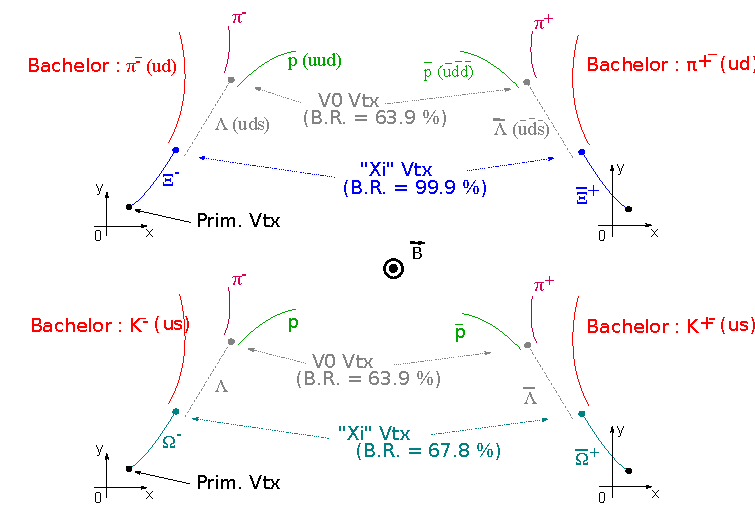
\includegraphics[width=0.75\linewidth]{images/cascDecay.pdf}
    \\
    \caption{Decay topology for charged cascade candidates $\Xi^{\pm}$ and $\Omega^{\pm}$\cite{Maire:2011}}
    \label{fig:cascDecay}
\end{figure}

The short decay length of the cascades is insufficient for direct observations in the ITS (with the closest SPD layer 3.9 cm from the interaction point).
Therefore, the cascade candidates are reconstructed with the help of the charged bachelor tracks and V0 daughter tracks. A two-step reconstruction
procedure employing $\Lambda$ reconstruction from the V0 daughter tracks and cascade candidate reconstruction using the reconstructed $\Lambda$ and an
associated bachelor track is implemented. Various kinematic and geometric selection criteria based on the decay topologies are used for deciding the
cascade candidates and eliminating combinatorial background, as outlined in Section \ref{sec:casc}.

\section{Data Sample}
The analysis is conducted on data obtained from proton-lead (p-Pb) collisions at $\sqrt{s_{\textnormal{\sc nn}}}$ = 8.16 TeV collected by the ALICE detector during
LHC's Run 2 phase in 2016. The particular dataset used for the analysis is internally referred to as "LHC16r\_pass2 \_CENT\_wSDD". The current analysis has been
performed on 6 runs marked as 'Good' in the Run Coordination Table: 265594, 265596, 265607, 266316, 266317 and 266318. They have been selected because of
relatively low interaction rates (<50 kHz) indicating low out-of-bunch pileup. These runs represent about 40\% of the total statistics available for this
period. The full processed statistics for the analysis comprises of $15.7 \times 10^{6}$ events.

The data sample is available as AOD files on CERN's computing network. The analysis code is written in CERN's software framework for data analysis: ROOT 6,
in conjunction with AliRoot libraries from the ALICE team. The analysis was performed on CERN's GRID network.

\section{Event selection criteria}

Basic event selection criteria following ALICE convention for p-Pb collisions were applied in this analysis. The event selection performed include $\colon$

\begin{itemize}
    \item \textbf{Minimum-bias trigger}: The minimum bias trigger aims to select only inelastic events, excluding collisions with residual gas in the beam pipe.
          This requires at least one hit (non-zero signal) in the VZERO detector on both sides of the collision (VZERO-A and VZERO-C).
    \item \textbf{Primary Vertex position}: Events with primary vertex within $|z|<10$ cm from the center of the detector along the $z$-axis were chosen.
    \item \textbf{INEL>0 event selection}: Only events with at least one reconstructed SPD tracklet in the $|\eta|$ < 1.0 range were selected for analysis.
    \item \textbf{Event multiplicity selection}: Due to the assymetric nature of the collision, the multiplicity estimator based on the VZERO-A amplitude was
          selected (Pb-going direction).
\end{itemize}

Moreover, event multiplicity classes to maximise the multplicity bins that could be explored with the present statistics were chosen. The classes are
enlisted in Table \ref{tab:multi}, with 0-5\% representing the highest multiplicities and 80-100\% ($\Xi^{\pm}$) or 60-100\% ($\Omega^{\pm}$) representing
the lowest multiplicities.

\begin{table}[H]
    \centering
    \begin{tabular}{|l|l|}
        \hline
        \textbf{Particle} & \textbf{V0A multiplicity classes (\%)}                             \\ \hline
        $\Xi^{\pm}$       & 0-5, 5-10, 10-15, 15-20, 20-30, 30-40, 40-50, 50-60, 60-80, 80-100 \\ \hline
        $\Omega^{\pm}$    & 0-5, 5-15, 15-30, 30-60, 60-100                                    \\ \hline
    \end{tabular}
    \caption{V0A multiplicity classes for cascades}
    \label{tab:multi}
\end{table}
The remaining sample after application of aforementioned event selection criteria had $11.2 \times 10^{6}$ events.

\section{Cascade candidates selection}\label{sec:casc}

Cascade candidate selection based on the decay topology were applied to ensure geometrical characteristics of the tracks comply with expected decay
mechanism. Some topological variables are illustrated in Fig. \ref{fig:topo}.

\begin{figure}[H]
    \centering
    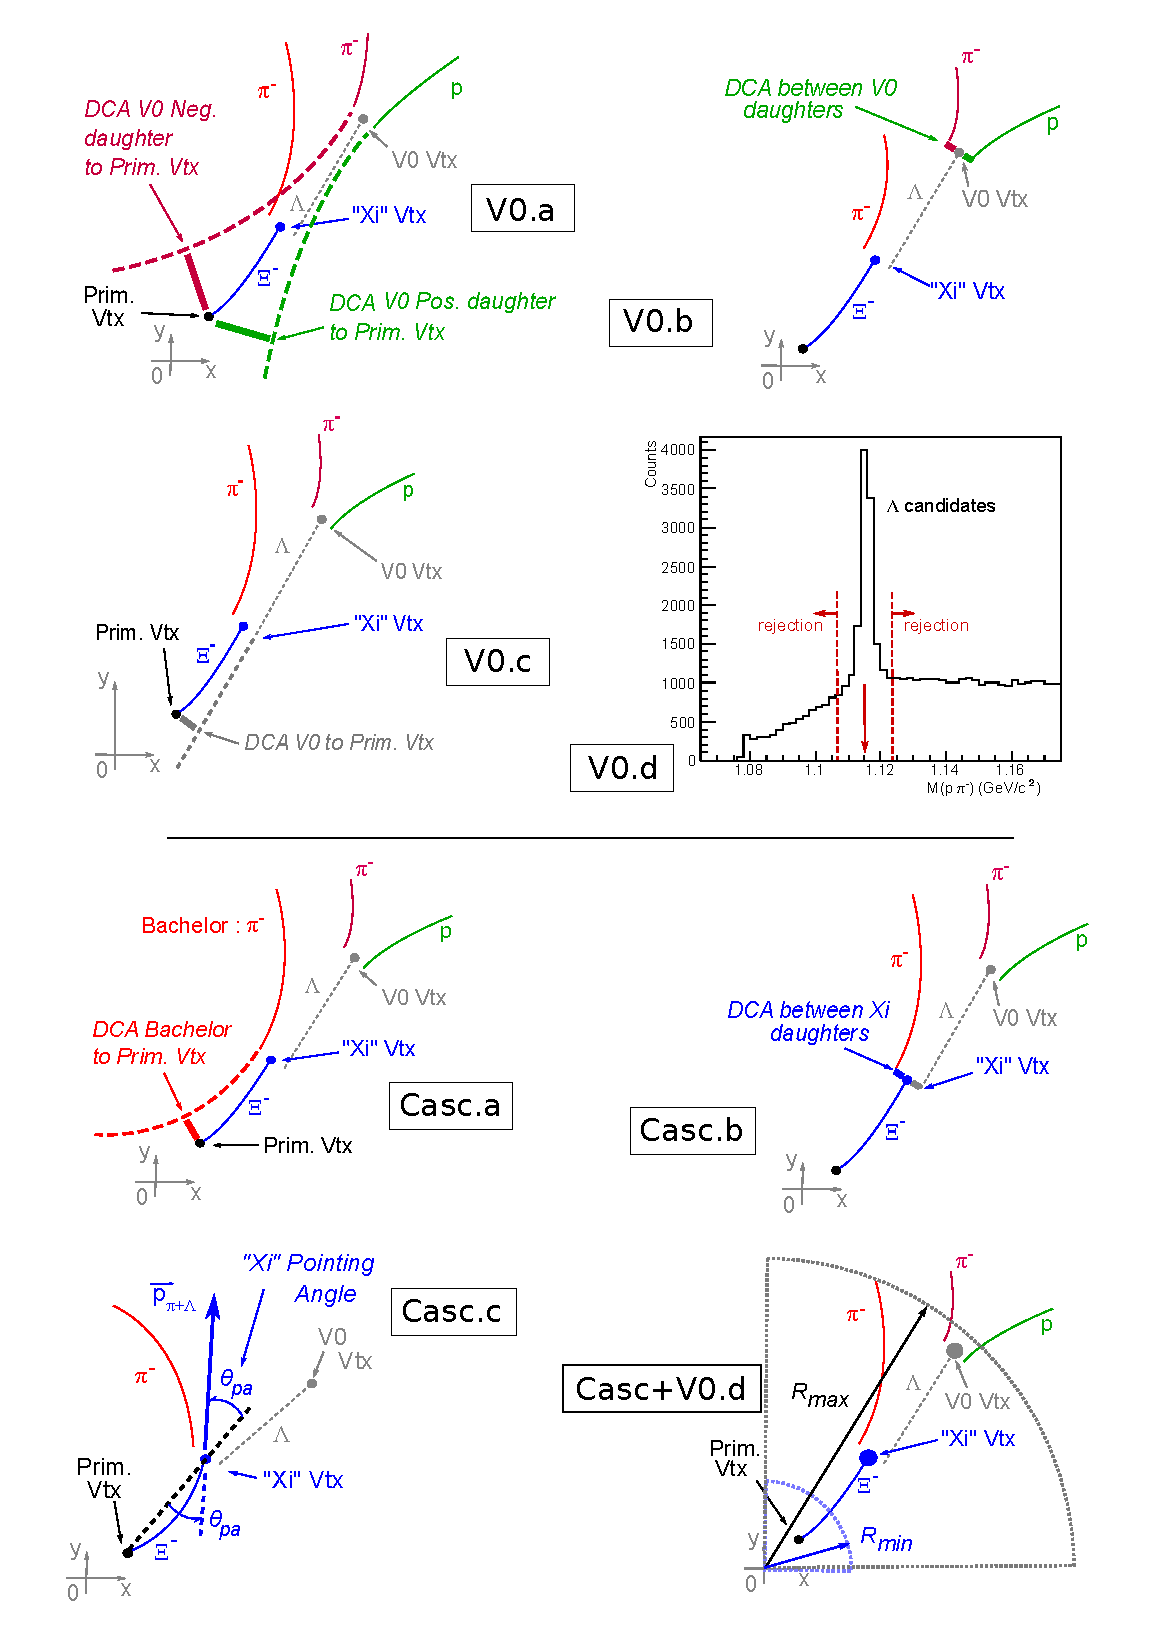
\includegraphics[clip,trim={0 0 0 14.3cm}, width=0.75\linewidth]{images/topologoical.pdf}
    \\
    \caption{Topological variables for cascades\cite{MaireTop:2011}}
    \label{fig:topo}
\end{figure}

\begin{itemize}
    \item \textbf{Rapidity interval}: The chosen rapidity interval for the analysis is -0.5 < y <0 corresponding to central rapidity region in p-Pb
          collisions.
    \item \textbf{Proper lifetime}: A proper lifetime selection of $\frac{mL}{p} < 3\times c\tau$ is applied, where $m$ denotes the cascade mass, $L$ is the
          cascade's decay length, $p$ is its total momentum and $c\tau$ is the lifetime (values in Table \ref{tab:cascades}). This helps to remove track combinations
          from low-momentum candidates originating unusually far from the Primary Vertex (PV).
    \item \textbf{TPC $\textbf{d}E/\textbf{d}x$ selection}: A cut on TPC's energy loss $\textnormal{d}E/\textnormal{d}x$
          is applied to remove background combinations of tracks from wrong particle species. Acceptance range of $4\sigma$
          is tolerated for cascade candidate's three daughter tracks.
    \item \textbf{Competing cascade rejection}: There is a significant background contribution from $\Xi^{\pm}$ decays
          while conducting the $\Omega^{\pm}$ analyses. To eliminate this background, it is necessary for the mass under
          $\Xi^{\pm}$ hypothesis to differ by at least 8 MeV/$c^{2}$ from the corresponding PDG mass.

    \item \textbf{Number of TPC clusters}: A minimum of 70 TPC clusters requirement is imposed to select good quality tracks.

\end{itemize}

All selection criteria involved in this analysis are listed in Table \ref{tab:crit}.

\begin{table}[H]
    \centering
    \begin{tabular}{|l|r|}
        \hline
        \textbf{Topological Variable}                          & \textbf{$\Xi (\Omega)$ Cut}             \\
                                                               & low, mid, high $p_{\textnormal{\sc t}}$ \\ \hline
        \hline

        Cascade transv. decay radius $R_{\textnormal{\sc 2d}}$ & >0.6 (0.5) cm                           \\ \hline
        V0 transv. decay radius                                & >1.2 (1.1) cm                           \\ \hline
        DCA (bachelor - PV)                                    & >0.04 cm                                \\ \hline
        DCA (V0 - PV)                                          & >0.06 cm                                \\ \hline
        DCA (meson V0 track - PV)                              & >0.04 cm                                \\ \hline
        DCA (baryon V0 track  - PV)                            & >0.03 cm                                \\ \hline
        DCA (V0 tracks)                                        & <1.7, 1.6, 1.5 $\sigma$                 \\ \hline
        DCA (bachelor - V0)                                    & <1.6, 1.5, 1.4 cm                       \\ \hline
        Cascade $\cos(PA)$                                     & >0.96, 0.97, 0.97                       \\ \hline
        V0 $\cos(PA)$                                          & >0.98 (0.97, 0.98, 0.98)                \\ \hline
        V0 invariant mass window                               & $\pm 0.008$ GeV/$c^{2}$                 \\ \hline
        \hline
        \textbf{Selection}                                     & \textbf{$\Xi (\Omega)$ Cut}             \\ \hline
        \hline
        Rapidity Interval                                      & -0.5 < $y$ < 0                          \\ \hline
        TPC $\textnormal{d}E/\textnormal{d}x$ selection        & < 4$\sigma$                             \\ \hline
        Proper lifetime ($\frac{mL}{p}$)                       & $< 3\times c\tau$                       \\ \hline
        Daughter Track $N_{\textnormal{TPC clusters}}$         & $\geq$ 70                               \\ \hline
        Competing cascade rejection (only $\Omega$)            & $|M(\Xi)-1.321| > $ 8 MeV/$c^{2}$       \\ \hline
        Tracking flags for daughters                           & kTPCrefit                               \\ \hline
    \end{tabular}
    \caption{Selection criteria for $\Xi^{\pm}$ and $\Omega^{\pm}$ candidates}
    \label{tab:crit}
\end{table}

The $p_{\textnormal{\sc t}}$ bin ranges used for the analysis divided into low, mid and high $p_{\textnormal{\sc t}}$ categories are listed in Table \ref{tab:pt}:

\begin{table}[H]
    \centering
    \begin{tabular}{|l||r|r|r|}
        \hline
        \multirow{2}{*}{\textbf{Particle}} & \multicolumn{3}{c|}{\textbf{$p_{\textnormal{\sc t}}$ bins (GeV/$c$)}}                                                         \\ \cline{2-4}

                                           & Low                                                                   & Mid                         & High                    \\ \hline \hline
        $\Xi^{\pm}$                        & \{0.8,1.1,1.3,1.5,1.7,1.9\}                                           & \{1.9,2.1,2.3,2.5,2.7,2.9\} & \{2.9,3.1,3.5,4.0,5.5\} \\ \hline
        $\Omega^{\pm}$                     & \{0.9,1.6,2.0\}                                                       & \{2.0,2.4,2.9\}             & \{2.9,3.5,5\}           \\ \hline
    \end{tabular}
    \caption{$p_{\textnormal{\sc t}}$ bin ranges used in analysis}
    \label{tab:pt}
\end{table}

\section{Signal Extraction}
Cascade invariant mass is calculated according to multiplicity classes and transverse momentum ranges for signal extraction. The $p_{\textnormal{\sc t}}$
bin ranges used allow for a spread of $p_{\textnormal{\sc t}}$ to be observed yet making sure that enough statistics are available for good signal extraction.
Table \ref{tab:pt} lists the momentum bin ranges while table \ref{tab:multi} lists the multiplicity classes. The binning for momentum ranges does not start
at zero since low momentum cascade decay particles, having lower radius of curvature, fail to traverse the detectors and hence, are not measured.
Particle-antiparticle
combinations have also been plotted for better statistics alongside singular particle plots, and  they are consistent with each other while improving
fitting characteristics in ranges with low statistics.

Thus, invariant mass plots are generated for each multiplicity and $p_{\textnormal{\sc t}}$ bin. In order to extract signal from the plots, the signal
region is fitted with a Gaussian + $2^{nd}$ degree polynomial fit and peak mean ($\mu$) and width($\sigma$) are estimated. Knowing these parameters,
the signal region, also known as the peak window, can be defined. For this analysis, the peak window was deduced to be:

\begin{equation}
    (M-4\sigma) \to (M+4\sigma)
\end{equation}


where $M$ is the position of peak($\mu$) value, denoting the particle mass, and is in agreement with the PDG mass. In the signal region, bin counting
technique is used to sum up signal + background counts.

For background estimation, a linear fit was chosen owing to a mostly flat background curve. The interval chosen for linear fitting of the background is
wider than the peak window and excludes the signal region completely:

\begin{equation}
    (M-8\sigma) \to (M-4\sigma) \  ; \    (M+4\sigma) \to (M+8\sigma)
\end{equation}

This two-part fitting interval lies outside the signal region and gives a more accurate background estimation curve, especially in case of low statistics.
This background fit is then integrated in the signal region, i.e. $(M-4\sigma) \to (M+4\sigma)$, in order to calculate background contribution
to the signal peak. Finally, the signal extraction is achieved by subtracting the value of this background fit integral calculated for area under the peak
from the bin counting of signal + background in the peak window. Figure \ref{fig:sigeg} gives an example of signal extraction performed on the invariant
mass spectra for $\Xi^{+}$ and $\Omega^{-}$.

\begin{figure}[H]
    \centering
    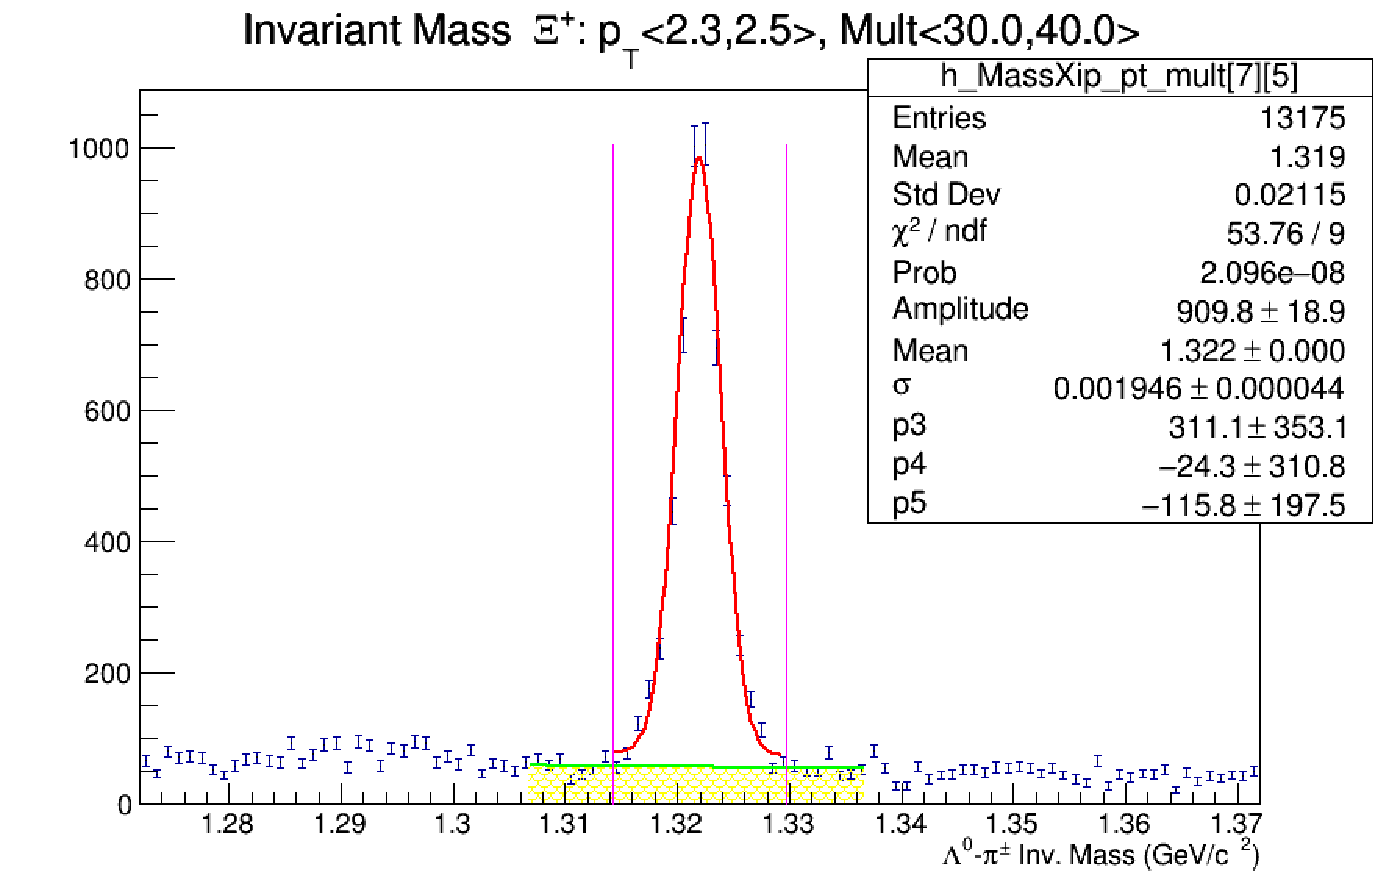
\includegraphics[width=0.75\linewidth]{images/xip_7_5.pdf}
    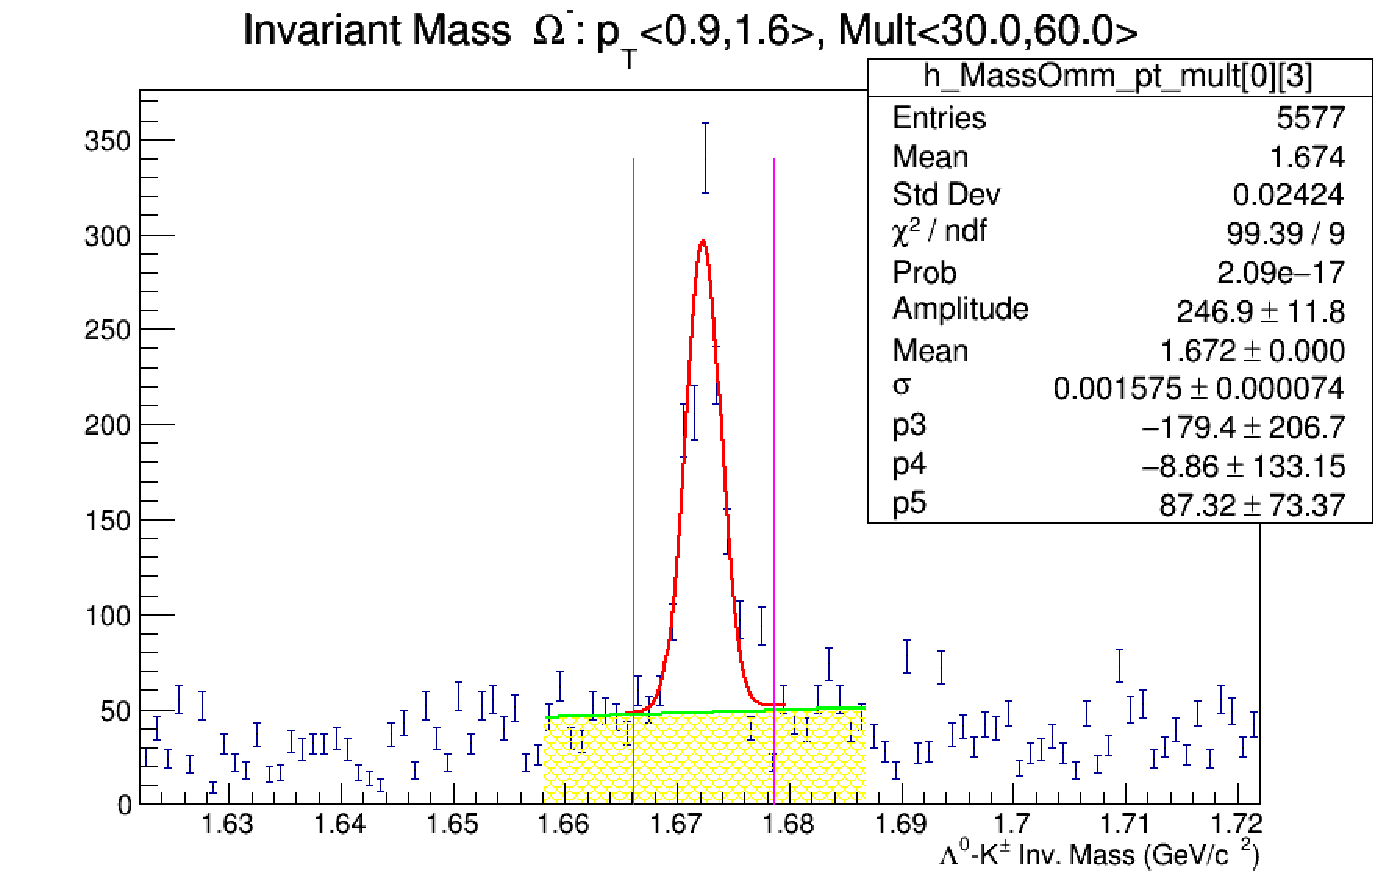
\includegraphics[width=0.75\linewidth]{images/omm_0_3.pdf}
    \caption{Plots showing examples of invariant mass for $\Xi^{+}$ (top) and $\Omega^{-}$ (bottom). $y$-axis denotes counts.}
    \label{fig:sigeg}
\end{figure}

In Figure \ref{fig:sigeg}, the red curve denotes Gaussian + $2^{nd}$ degree polynomial fit for the signal and the green curve denotes the linear fit of the
background, fitted for the region beyond the magenta lines. The peak window is encapsulated by the two vertical magenta lines. For background subtraction,
the area highlighted in yellow under the peak is used, limited by the vertical magenta lines.

\section{Raw transverse momentum spectra}

Using the procedure mentioned in the previous section, raw transverse momentum spectra ($p_{\textnormal{\sc t}}$) for $\Xi^{\pm}$ and $\Omega^{\pm}$ along
with particle anti-particle combination spectra were obtained and are shown in figure \ref{fig:rawpt} for different V0A multiplicity classes.

\begin{figure}[H]
    \centering
    \begin{subfigure}{.5\textwidth}
        \centering
        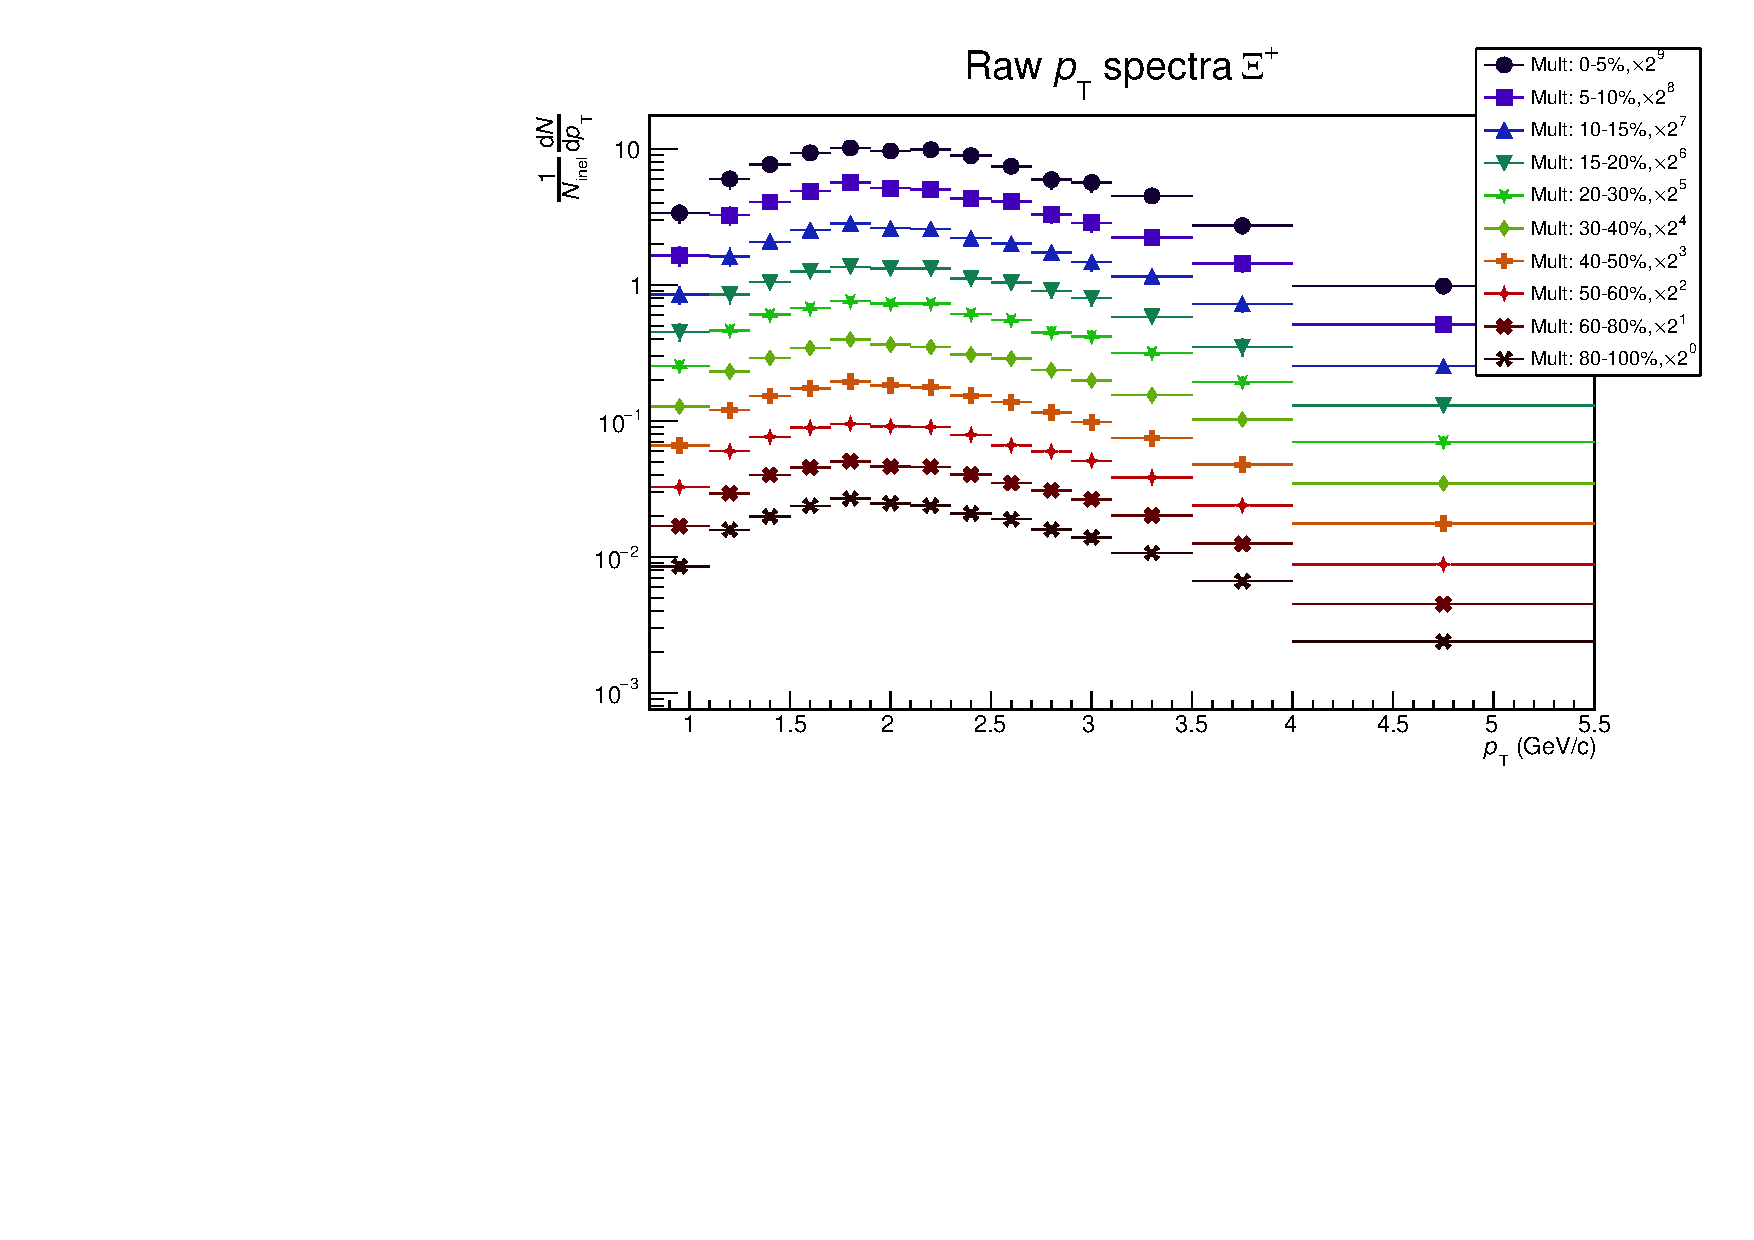
\includegraphics[width=\linewidth]{images/raw_xip.pdf}
    \end{subfigure}%
    \begin{subfigure}{.5\textwidth}
        \centering
        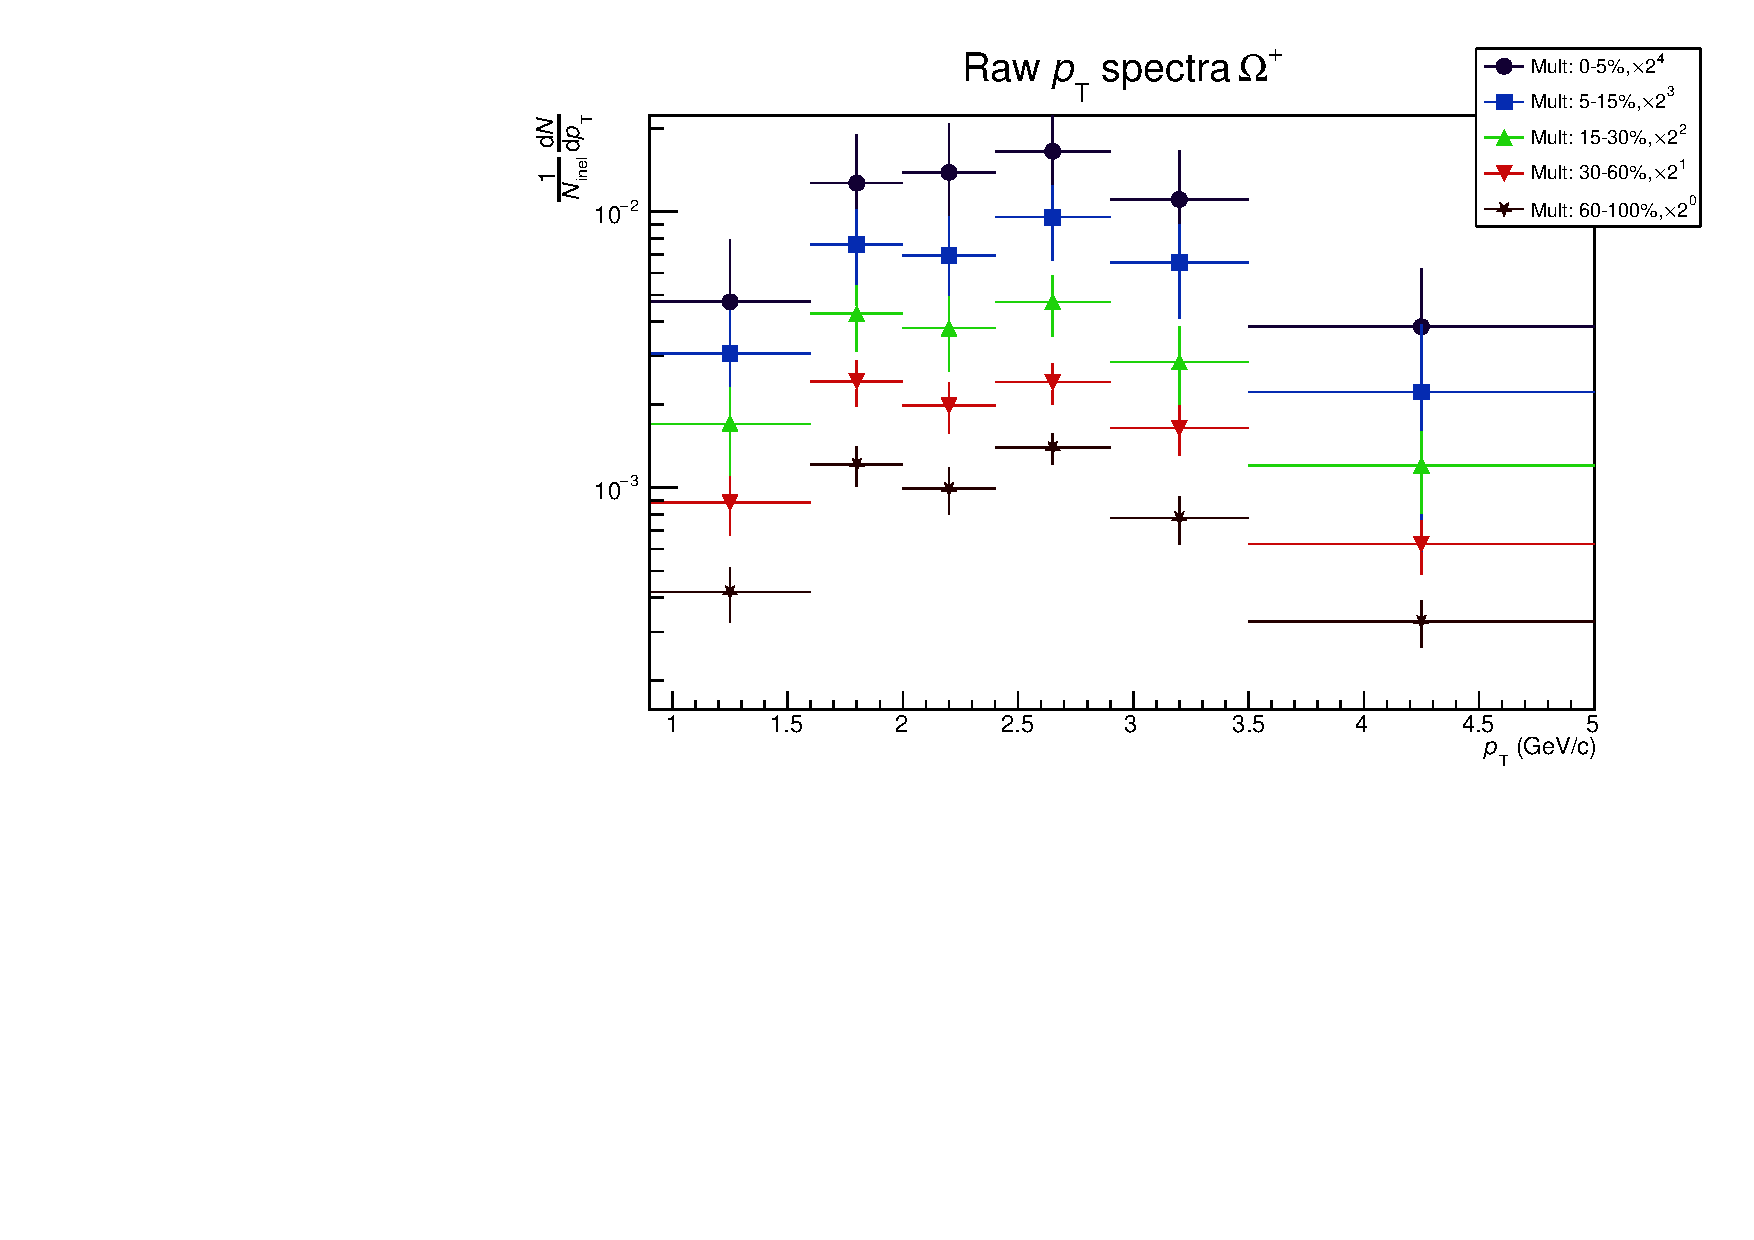
\includegraphics[width=\linewidth]{images/raw_omp.pdf}
    \end{subfigure}

    \medskip
    \begin{subfigure}{.5\textwidth}
        \centering
        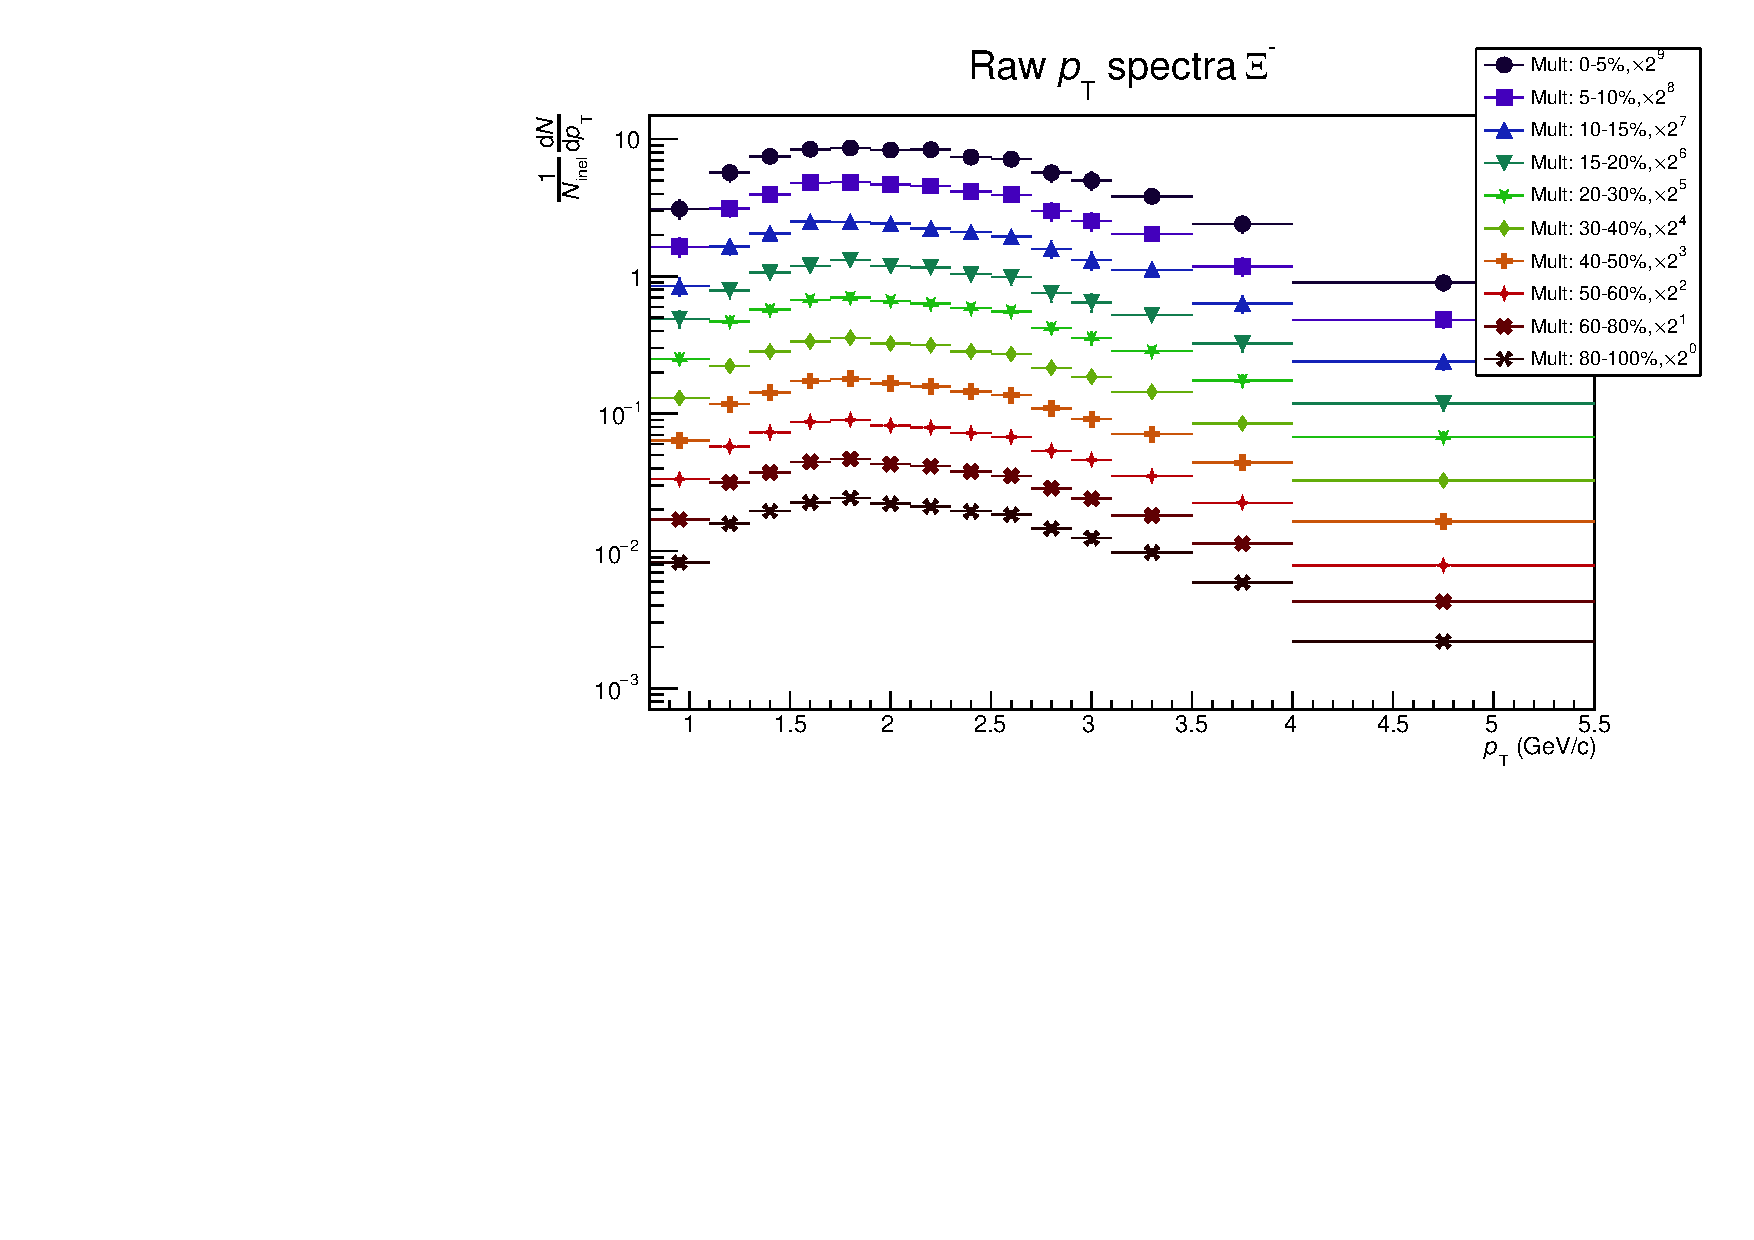
\includegraphics[width=\linewidth]{images/raw_xim.pdf}
    \end{subfigure}%
    \begin{subfigure}{.5\textwidth}
        \centering
        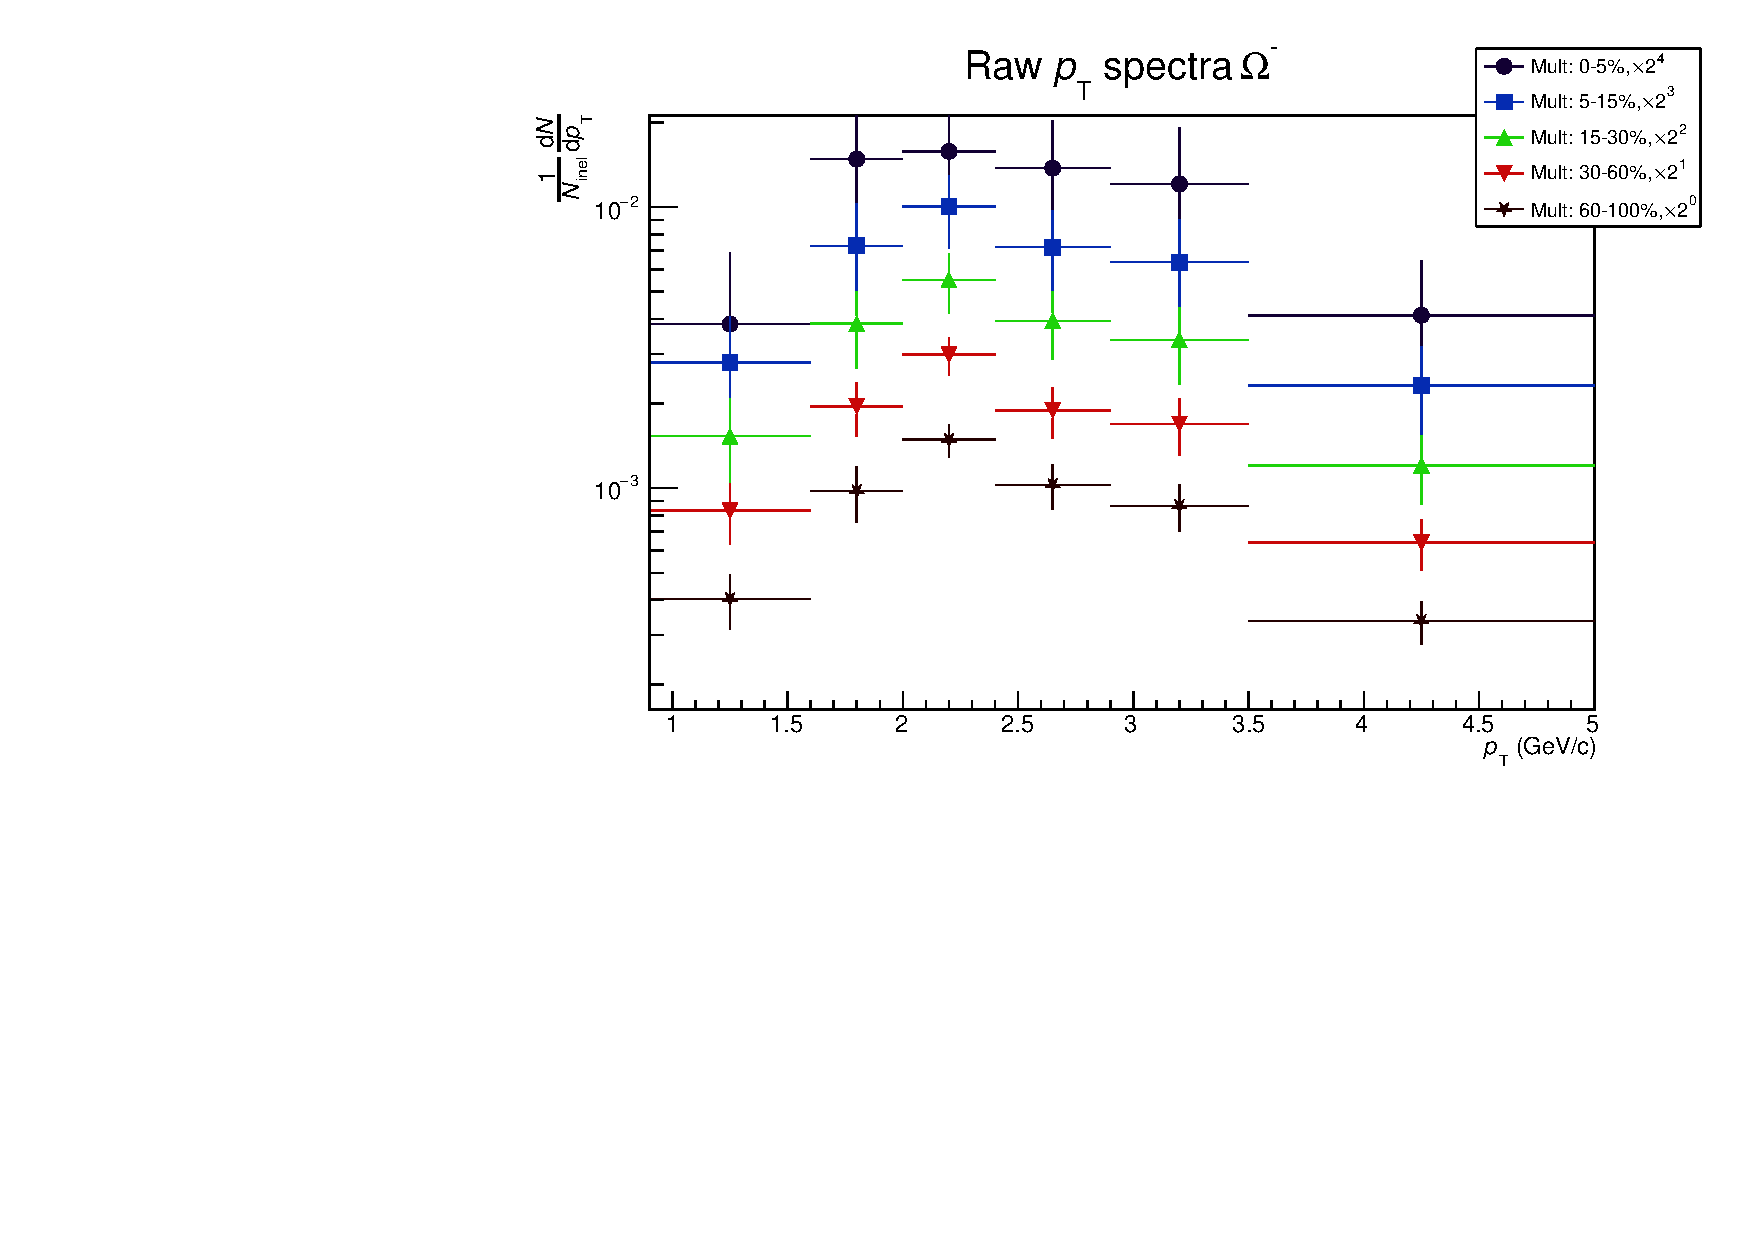
\includegraphics[width=\linewidth]{images/raw_omm.pdf}
    \end{subfigure}

    \medskip
    \begin{subfigure}{.5\textwidth}
        \centering
        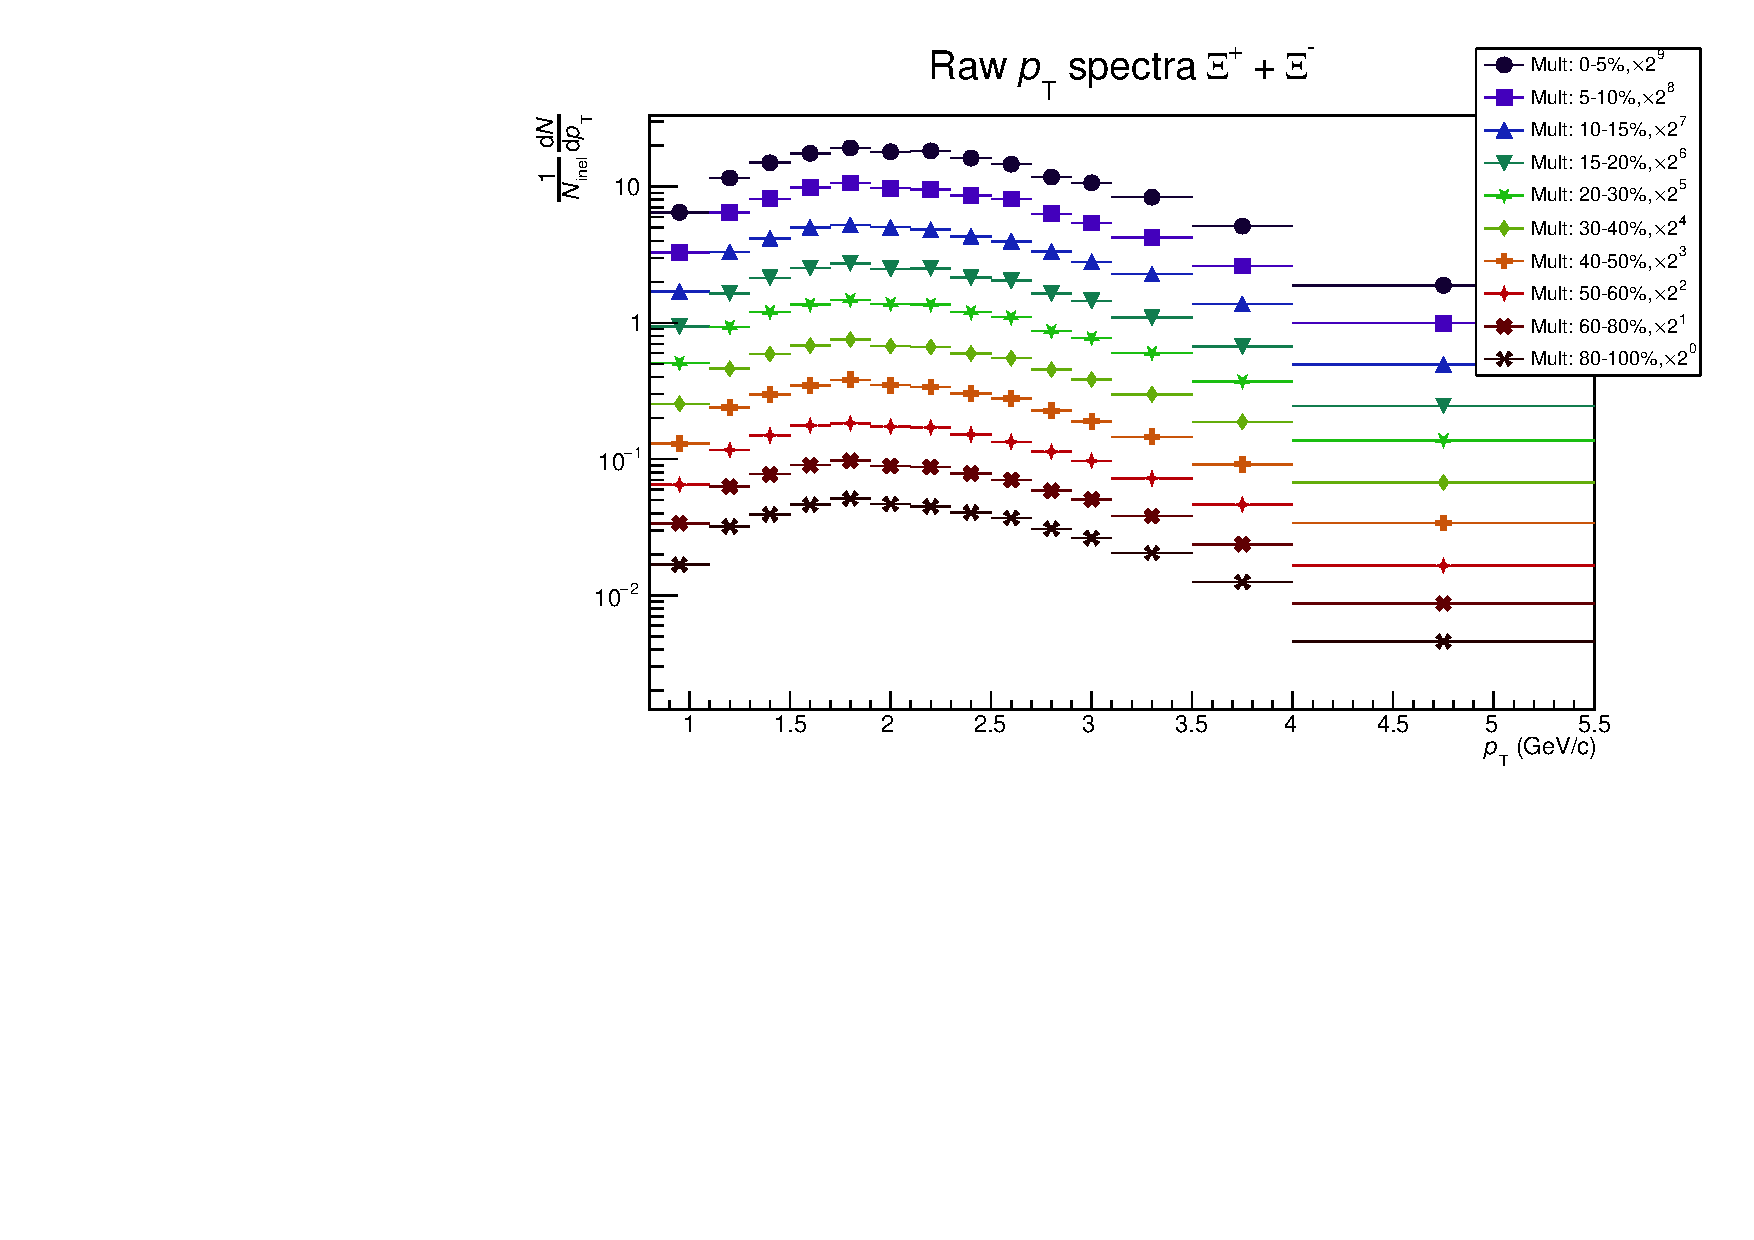
\includegraphics[width=\linewidth]{images/raw_xiC.pdf}
    \end{subfigure}%
    \begin{subfigure}{.5\textwidth}
        \centering
        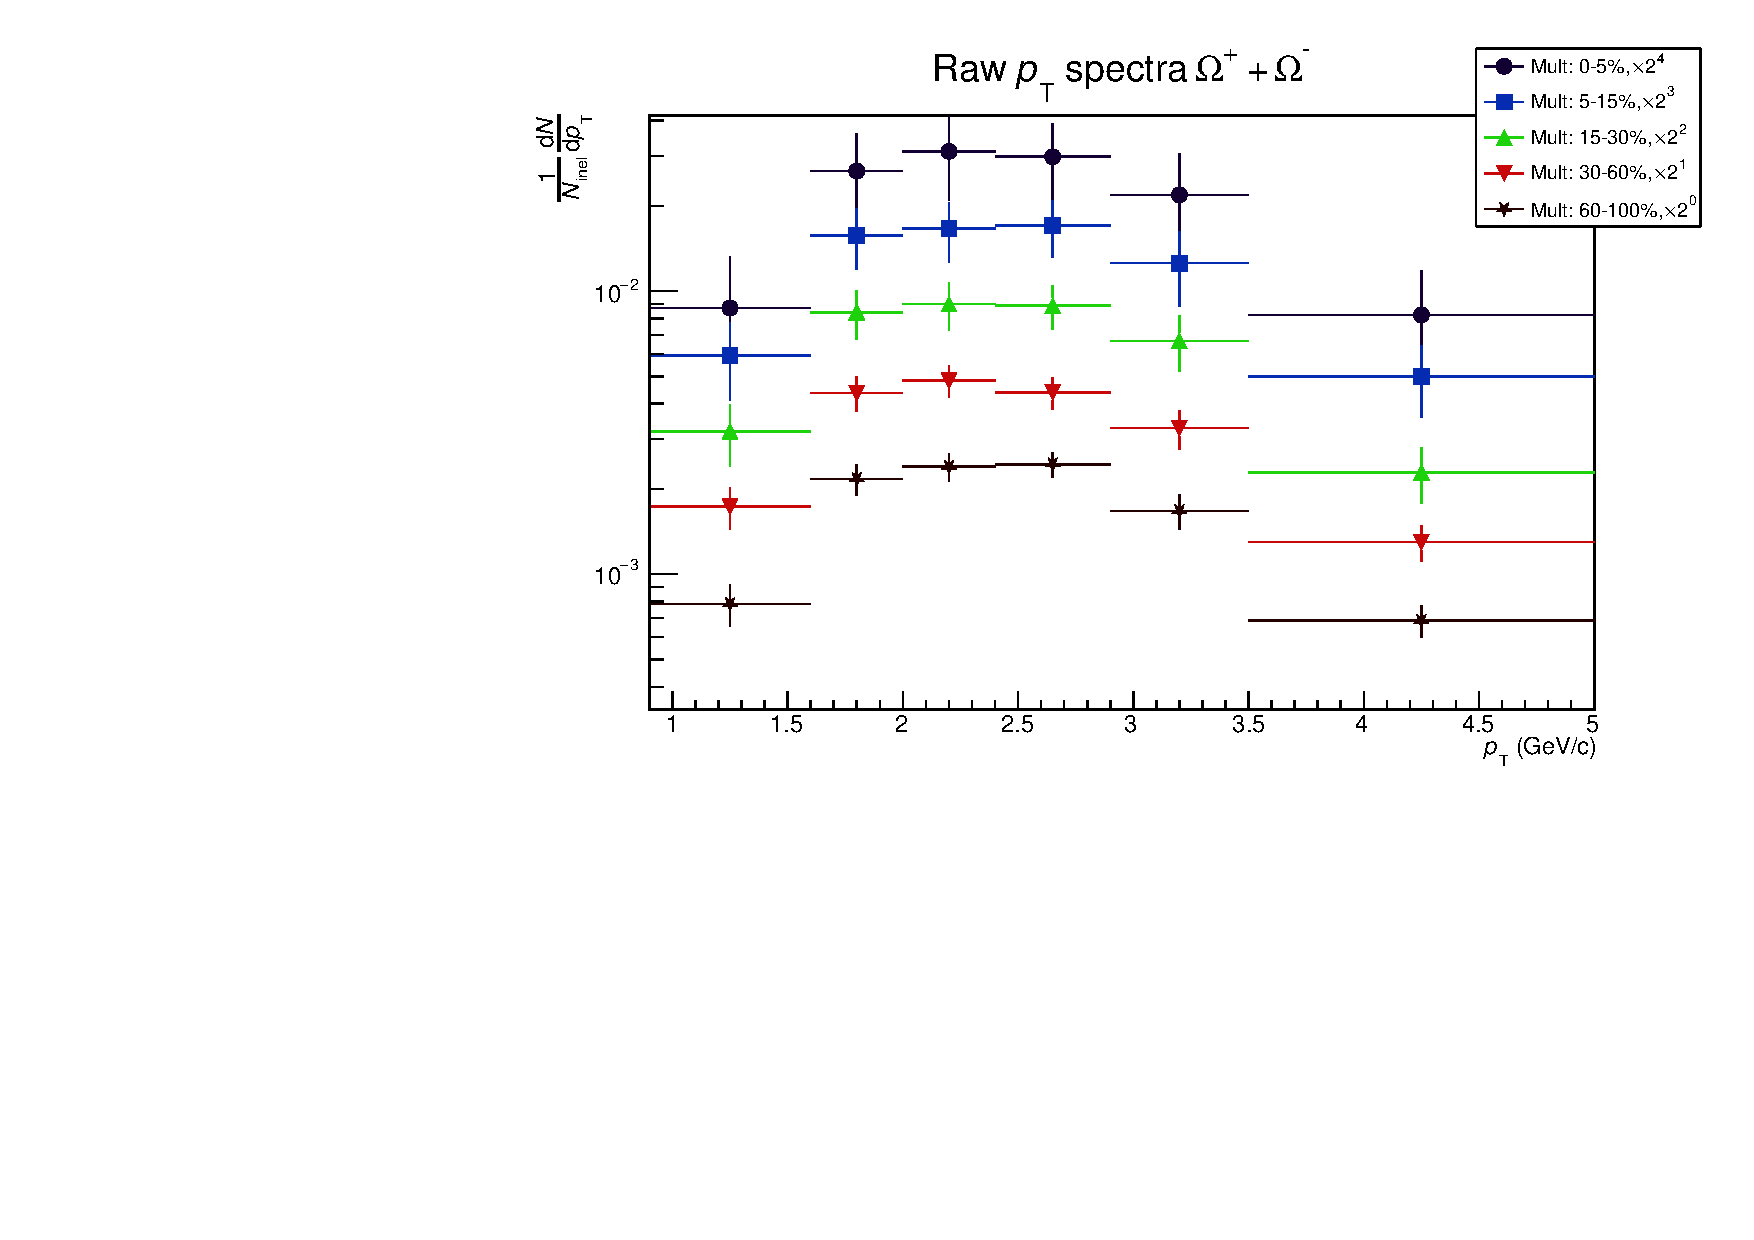
\includegraphics[width=\linewidth]{images/raw_omC.pdf}
    \end{subfigure}
    \caption{Plots depicting raw ($p_{\textnormal{\sc t}}$) spectra for $\Xi^{\pm}$ (left) and $\Omega^{\pm}$ (right)}
    \label{fig:rawpt}
\end{figure}

In figure \ref{fig:rawpt}, the left side denotes the raw transverse momentum spectra for $\Xi^{\pm}$ and the right side for $\Omega^{\pm}$. The top
figures are for the positively charged particle spectra, middle for negatively charged and the bottom ones as a combination of the two.
\chapter{Outlook}
In this work, the results for raw transverse momentum spectra for charged cascade particles $\Xi^{\pm}$ and $\Omega^{\pm}$ in proton-lead collisions at
$\sqrt{s_{\textnormal{\sc nn}}}$ = 8.16 TeV in ALICE were presented.

Developing a basic theoretical understanding supported by experimental results pertaining to Quark-Gluon Plasma and its signatures were described. A brief
overview of the experimental setup and the detector assemblies relevant to the analysis was also detailed. This was followed by details of the analysis,
including data collection and reconstruction, data sample selection, event and candidate selection criteria, and an explanation of the signal extraction
method employed in this analysis. The optimised selection criteria was tabulated and raw (uncorrected) transverse momentum spectra for the cascade particles
distributed over different multiplicity classes and $p_{\textnormal{\sc t}}$ ranges was shown.

Future aspects of this work include pile-up estimation and correction using all available data samples in this dataset, detector efficiency estimation and
acceptance corrections using the Monte Carlo productions and obtaining the efficiency-corrected transverse momentum spectra. This spectra can be
compared to available $\Xi^{\pm}$
and $\Omega^{\pm}$ $p_{\textnormal{\sc t}}$ spectra in p-Pb collisions at different energies. Finally, systematic uncertainties estimation for chosen selection
criteria and error estimation will be performed.



\chapter*{Súhrn}
V tejto práci boli prezentované nekorigované spektrá priečnych hybností nabitých častíc $\Xi^{\pm}$ a $\Omega^{\pm}$ v zrážkach protónov s olovom pri 
$\sqrt{s_{\textnormal{\sc nn}}}$ = 8,16 TeV v experimente ALICE na Veľkom hadrónovom zrážači (LHC) v CERN.

Kvalitatívne boli opísané teoretické základy pre pochopenie fyziky kvarkovo-gluónovej plazmy (QGP) a uvedený stručný prehľad niektorých experimentálnych 
signatúr QGP. Bol opísaný detektorový systém experimentu ALICE so zameraním na kľúčové detektory potrebné pre rekonštrukciu rozpadov nabitých multipodivných 
hyperónov. Nasledoval podrobný opis analýzy dát -- výber vhodných zrážok, výber selekčných kritérií pre kandidátov na rozpad a popis extrakcie signálu z 
rozdelenia invariantných hmotností rozpadových produktov. Finálne selekčné kritériá boli uvedené v tabuľke a nekorigované spektrá priečnych hybností multipodivných 
hyperónov $\Xi^{\pm}$ a $\Omega^{\pm}$ boli zobrazené pre jednotlivé multiplicitné triedy.

V budúcnosti bude analýza rozšírená o korekciu príspevku z tzv. pile-up eventov (t.j. viac zrážok zrekonštruovaných ako jedna zrážka), budú pridané datasety 
s vyššou frekvenciou zrážok a teda s vyšším obsahom pile-up eventov. Pomocou zrekonštruovaných Monte Carlo dát bude odhadnutá korekcia na detektorovú akceptanciu 
a účinnosť rekonštrukcie kaskádnych rozpadov $\Xi^{\pm}$ a $\Omega^{\pm}$. Nakoniec budú odhadnuté systematické chyby z rôznych uvažovaných zdrojov.

Výsledné korigované spektrá priečnych hybností nabitých častíc $\Xi^{\pm}$ a $\Omega^{\pm}$ budú porovnané so spektrami z p-Pb zrážok avšak pri inej zrážkovej 
energii. Taktiež budú porovnané s inými zrážkovými systémami, ako napr. vysokomultiplicitné protón-protónové zrážky alebo Pb—Pb zrážky v závislosti od multiplicity 
nabitých častíc v evente.



\bibliographystyle{unsrtnat}
\bibliography{references}
\end{document}
